\chapter{Metodologia}\label{metodologia}

\section{Modelagem estatística para dados PolSAR}\label{cap_acf_sec1}
Os sistemas SAR totalmente polarimétricos transmitem pulsos de micro-ondas polarizados ortogonalmente e medem componentes ortogonais do sinal recebido. Para cada pixel, a medida resulta em uma matriz de coeficientes de espalhamento. Esses coeficientes são números complexos que descrevem no sistema SAR a transformação do campo eletromagnético transmitido para o campo eletromagnético recebido.

A transformação pode ser representada como
\begin{equation*}
 \left[
\begin{array}{c}
	E_\text{h}^\text{r}   \\
	E_\text{v}^\text{r}    \\
\end{array}
\right]
 = \frac{e^{\hat{\imath} \text{kd}}}{\text{d}}\left[
\begin{array}{cc}
	S_{\text{hh}}   & S_{\text{hv}}   \\
	S_{\text{vh}}   & S_{\text{vv}}   \\
\end{array}
\right]
 \left[
\begin{array}{c}
	E_\text{h}^\text{t}   \\
	E_\text{v}^\text{t}   \\
\end{array}
\right],
\end{equation*}
onde k denota o número de onda, $\hat{\imath}$ é um número complexo e d é a distância entre o radar e o alvo. No campo eletromagnético com componentes $E_\text{i}^\text{j}$, o índice subscrito denota polarização horizontal (h) ou vertical (v), e o índice sobrescrito indica a onda recebida (r) ou transmitida (t). 

A matriz de espalhamento complexa $\mathbf{S}$ é definida por
\begin{equation}\label{matriz_de_espalhamento}
\mathbf{S} = \left[
\begin{array}{cc}
	S_{\text{hh}}   & S_{\text{hv}}   \\
	S_{\text{vh}}   & S_{\text{vv}}   \\
\end{array}
\right],
\end{equation}
onde as entradas da matriz $S_{\text{i,j}}$ são os coeficientes de espalhamento complexo, tal que os índices i e j são associados ao  recebimento e a transmissão das ondas, por exemplo, o coeficiente de espalhamento $S_{\text{hv}}$ está associado a onda transmitida na direção vertical (v) e recebida na direção horizontal (h).

Definindo a diagonal principal da matriz de espalhamento por co-polarização pois relaciona a polarização das ondas transmitidas e recebidas nas mesmas direções, e a os elementos da diagonal secundária da matriz de espalhamento por polarização cruzada relacionando os estados de polarizações ortogonais.
% ver~\citep{lp}.
 
A matriz $\mathbf{S}$ depende da definição do sistema de coordenadas, se a antena transmissora e receptora de sinal estão localizadas na mesma posição consideramos as medidas mono estáticas e consideramos o sistema de coordenada \textbf{BSA} - \textit{Back Scattering Alignment}, desta forma o sistema de coordenadas da transmissão e recepção de sinal são coincidentes.   
 
A potência total espalhada no caso de um sistema de radar polarimétrico é o chamado \textit{span}, sendo definido no caso mais geral como,
\begin{equation}\label{span_geral}
\mathbf{Span(S)} = \traco(SS^H)=|S_{hh}|^2+|S_{hv}|^2|+|S_{vh}|^2+|S_{vv}|^2,
\end{equation}
onde o operador $\traco(\cdot)$ é o traço de uma matriz.


\subsection{Matriz de coerência polarimétrica de Pauli ($T_4$) e matriz de covariância lexicográfica ($C_4$)}
A matriz de espalhamento $\mathbf{S}$ pode ser representada pela construção do vetor,
\begin{equation}\label{def_vet_espalhamento}
\mathbf{k}=\frac{1}{2}\left[\traco(S\Psi_1)\quad\traco(S\Psi_2)\quad \traco(S\Psi_3)\quad \traco(S\Psi_4)\right]^T,
\end{equation}
onde $\{\Psi_i\}_{i=1}^4$ é uma base para o espaço das matrizes hermitianas $2\times 2$.

Diferentes bases para o mesmo espaço matricial podem ser definidas, no presente trabalho serão consideradas duas bases chamadas respectivamente de  base de Pauli e base lexicográfica, a  base de Pauli é definida por,
\begin{equation}\label{base_de_pauli}
\{\Psi_P\} = \left\{
\sqrt{2}\left[\begin{array}{cc}
	1  & 0  \\
	0  & 1 \\
\end{array}\right],
\sqrt{2}\left[\begin{array}{cc}
	1  & 0  \\
	0  & -1  \\
\end{array}\right],
\sqrt{2}\left[\begin{array}{cc}
	0  & 1  \\
	1  & 0  \\
\end{array}\right],
\sqrt{2}\left[\begin{array}{cc}
	0       & -i  \\
	i  & 0  \\
\end{array}\right]
\right\},
\end{equation}
e a base lexicográfica é definida como,
\begin{equation}\label{base_de_lexicografica}
\{\Psi_L\} = \left\{
2\left[\begin{array}{cc}
	1  & 0  \\
	0  & 0 \\
\end{array}\right],
2\left[\begin{array}{cc}
	0  & 1  \\
	0  & 0  \\
\end{array}\right],
2\left[\begin{array}{cc}
	0  & 0  \\
	1  & 0 \\
\end{array}\right],
2\left[\begin{array}{cc}
	0  & 0  \\
	0  & 1  \\
\end{array}\right]
\right\}.
\end{equation}

Usando as bases (\ref{base_de_pauli}), (\ref{base_de_lexicografica}) e  a definição do vetor (\ref{def_vet_espalhamento}) representamos a matriz de espalhamento pelo vetor característico de Pauli $4$-D,
\begin{equation}\label{vetor_pauli_4d}
\mathbf{k}= \frac{1}{\sqrt{2}}\left[
	\begin{array}{cccc}
	S_{hh} + S_{vv}& S_{hh} - S_{vv}& S_{hv} + S_{vh} &i (S_{hv} - S_{vh})   \\
\end{array}\right]^T=\frac{1}{\sqrt{2}}[k_1\quad k_2\quad k_3\quad k_4]
\end{equation}
e pelo vetor característico lexicográfico $4$-D 
\begin{equation}\label{vetor_lexicografico_4d}
\mathbf{\Omega}= \left[
	\begin{array}{cccc}
	S_{hh}& S_{hv} &S_{hv}& S_{vv}   \\
\end{array}\right]^T=[\Omega_1\quad \Omega_2\quad \Omega_3\quad \Omega_4]
\end{equation}

A matriz de espalhamento pode ser relacionada com os vetores (\ref{vetor_pauli_4d}) e (\ref{vetor_lexicografico_4d}) da seguinte maneira,
\begin{equation}\label{mat_esp_rel_pauli_lex}
\mathbf{S} = \left[
\begin{array}{cc}
	S_{hh}   & S_{hv}   \\
	S_{vh}   & S_{vv}   \\
\end{array}
\right]=
\left[
\begin{array}{cc}
	\Omega_1   & \Omega_2   \\
	\Omega_3   & \Omega_4   \\
\end{array}
\right]=\frac{1}{\sqrt{2}}
\left[
\begin{array}{cc}
	 k_1+k_2  & k_3-ik_4   \\
	 k_3+ik_4 & k_1-k_2   \\
\end{array}
\right]
\end{equation}

As constantes $2$ e $\sqrt{2}$ nas equações (\ref{base_de_pauli}) e (\ref{base_de_lexicografica}) servem para manter a norma dos vetores de espalhamento iguais independente da escolha das bases. O produto interno escolhido é o padrão para o espaço vetorial dos vetores complexos de dimensão 4.

Podemos assim garantir que a invariância da potência total 
\begin{equation}\label{span_invariante}
\begin{array}{ccc}
\mathbf{Span(S)} &=& \traco(SS^H)\\
	   &=&  \traco(SS^H)=|S_{hh}|^2+|S_{hv}|^2|+|S_{vh}|^2+|S_{vv}|^2  \\
	   &=&  \mathbf{k}^H\mathbf{k}=|\mathbf{k}|^2\\
	   &=& \mathbf{\Omega}^H\mathbf{\Omega}=|\mathbf{\Omega}|^2.
\end{array}
\end{equation}

A transformação linear unitária $U_{4(L \rightarrow P)}$ é definida como uma transformação que aplica o vetor na base lexicográfica em um vetor na base de Pauli. Definimos a notação \textrm{SU(4)} para designar a transformação  unitária
\begin{equation}\label{trans_matriz_unit_su4}
\frac{1}{\sqrt{2}}\left[
\begin{array}{c}
	  S_{hh} +  S_{vv}\\  
	  S_{hh} -  S_{vv}\\
	  S_{hv} +  S_{vh} \\
        i(S_{hv} -  S_{vh}) \\
\end{array}
\right]=\frac{1}{\sqrt{2}}	
\left[
\begin{array}{rrrr}
	1   & 0 & 0 & 1  \\
	1   & 0 & 0 & -1  \\
	0   & 1 & 1 & 0  \\
	0   & i & -i &0   \\
\end{array}
\right]
\left[
\begin{array}{c}
	S_{hh} \\  
	S_{hv} \\
	S_{vh} \\
	S_{vv} \\
\end{array}
\right]
\end{equation}
desta maneira definimos a matriz unitária,
\begin{equation}\label{matriz_unit_su4}
U_{4(L \rightarrow P)}=	\frac{1}{\sqrt{2}}	
\left[
\begin{array}{rrrr}
	1   & 0 & 0 & 1  \\
	1   & 0 & 0 & -1  \\
	0   & 1 & 1 & 0  \\
	0   & i & -i &0   \\
\end{array}
\right]
\end{equation}


Para o caso biestático definimos a matriz de coerência polarimétrica de Pauli 
\begin{equation}\label{matriz_polar_pauli}
	\mathbf{T}_4=\mathbf{k}\mathbf{k}^H=	
\left[
\begin{array}{rrrr}
	|k_1|^2       & k_1\bar{k}_2  & k_1\bar{k}_3  & k_1\bar{k}_4  \\
	k_2\bar{k}_1  & |k_2|^2       & k_2\bar{k}_3  & k_2\bar{k}_4  \\
	k_3\bar{k}_1  & k_3\bar{k}_2  &    |k_3|^2    & k_3\bar{k}_4  \\
	k_4\bar{k}_1  & k_4\bar{k}_2  & k_4\bar{k}_3  & |k_4|^2   \\
\end{array}
\right]
\end{equation}
e a matriz de covariância lexicográfica
\begin{equation}\label{matriz_covar_lexic}
	\mathbf{C}_4=\mathbf{\Omega}\mathbf{\Omega}^H=	
\left[
\begin{array}{rrrr}
	|\Omega_1|^2       & \Omega_1\bar{\Omega}_2  & \Omega_1\bar{\Omega}_3  & \Omega_1\bar{\Omega}_4  \\
	\Omega_2\bar{\Omega}_1  & |\Omega_2|^2       & \Omega_2\bar{\Omega}_3  & \omega_2\bar{\Omega}_4  \\
	\Omega_3\bar{\Omega}_1  & \Omega_3\bar{\Omega}_2  &    |\Omega_3|^2    & \Omega_3\bar{\Omega}_4  \\
	\Omega_4\bar{\Omega}_1  & \Omega_4\bar{\Omega}_2  & \Omega_4\bar{\Omega}_3  & |\Omega_4|^2   \\
\end{array}
\right]
\end{equation}

Usando as definções e as propriedades acima teremos
\begin{equation}\nonumber
\begin{array}{rrrrr}
	\mathbf{T}_4&=&\mathbf{k}\mathbf{k}^H&=&\mathbf{U_4\Omega}(\mathbf{U_4\Omega})^H	\\
	   &=&\mathbf{U_4\Omega}\mathbf{\Omega}^H\mathbf{U_4}^H&&	\\
	   &=&\mathbf{U_4}\mathbf{C}_4\mathbf{U_4}^H&=&\mathbf{U_4}\mathbf{C}_4\mathbf{U_4}^{-1}\\
\end{array}
\end{equation}
\begin{equation}\label{matriz_simil_t4_c4}
\begin{array}{rrr}
	 \mathbf{T}_4  &=&\mathbf{U_4}\mathbf{C}_4\mathbf{U_4}^{-1}\\
\end{array}
\end{equation}
com isso, podemos concluir que
\begin{equation}\label{traco_t4_c4}
\begin{array}{rrrrr}
	\traco({\mathbf{T}_4})  &=&\traco({\mathbf{C}_4})&=&\mathbf{Span(S)}.\\
\end{array}
\end{equation}

\subsection{Matriz de coerência polarimétrica de Pauli ($T_3$) e matriz de covariância lexicográfica ($C_3$)}

Podemos entender as interações da ondas eletromagnéticas em alvos naturais sob a ótica do teorema da reciprocidade que considera o meio reciproco, de uma maneira geral as propriedades de transmissão e recebimento de uma antena são idênticos. Então podemos definir a igualdade dos termos complexos (polarização cruzada) $S_{hv}=S_{vh}$.  Veja \citet{lp}. 

O entendimento para extrair informação da matriz de espalhamento $\mathbf{S}$ pode ser alcançado coma construção de um sistema de vetores. A matriz de espalhamento $\mathbf{S}$ pode ser representada pela construção do vetor,
\begin{equation}\label{def_vet_espalhamento_3d}
\mathbf{k}=\frac{1}{2}\left[\traco(S\Psi_1)\quad\traco(S\Psi_2)\quad \traco(S\Psi_3)\right]^T,
\end{equation}
onde $\{\Psi_i\}_{i=1}^3$ é uma base para o espaço das matrizes hermitianas $2\times 2$.

Neste trabalho serão consideradas duas bases para os espaço das matrizes nomeadas como base de Pauli e base lexicográfica.	

A base de Pauli pode ser definida como,
\begin{equation}\label{base_de_pauli_3d}
\{\Psi_P\} = \left\{
\sqrt{2}\left[\begin{array}{cc}
	1  & 0  \\
	0  & 1 \\
\end{array}\right],
\sqrt{2}\left[\begin{array}{cc}
	1  & 0  \\
	0  & -1  \\
\end{array}\right],
\sqrt{2}\left[\begin{array}{cc}
	0  & 1  \\
	1  & 0  \\
\end{array}\right]
\right\}.
\end{equation}

A base lexicográfica pode ser definida como,
\begin{equation}\label{base_de_lexicografica_3d}
\{\Psi_L\} = \left\{
2\left[\begin{array}{cc}
	1  & 0  \\
	0  & 0 \\
\end{array}\right],
2\sqrt{2}\left[\begin{array}{cc}
	0  & 1  \\
	0  & 0  \\
\end{array}\right],
2\left[\begin{array}{cc}
	0  & 0  \\
	0  & 1  \\
\end{array}\right]
\right\}.
\end{equation}

Usando as bases (\ref{base_de_pauli_3d}), (\ref{base_de_lexicografica_3d}) e a equação (\ref{def_vet_espalhamento_3d}) geramos os seguintes vetores de espalhamento que pode ser representada pelo vetor característico de Pauli $3$-D,
\begin{equation}\label{vetor_pauli_3d}
\mathbf{k}= \frac{1}{\sqrt{2}}\left[
	\begin{array}{ccc}
	S_{hh} + S_{vv} & S_{hh} - S_{vv}& 2S_{hv}   \\
\end{array}\right]^T=\frac{1}{\sqrt{2}}[k_1\quad k_2\quad k_3],
\end{equation}
e pelo vetor característico lexicográfico $3$-D 
\begin{equation}\label{vetor_lexicografico_3d}
\mathbf{\Omega}= \frac{1}{\sqrt{2}}\left[
	\begin{array}{ccc}
	S_{hh}& S_{hv}& S_{vv}   \\
\end{array}\right]^T=[\Omega_1\quad \Omega_2\quad \Omega_3].
\end{equation}

As constantes $2$ e $\sqrt{2}$ nas equações (\ref{base_de_pauli_3d}) e (\ref{base_de_lexicografica_3d}) servem para manter a norma dos vetores de espalhamento iguais independente da escolha das bases. O produto interno escolhido é o padrão para o espaço vetorial dos vetores complexos de dimensão 3.

Podemos assim garantir que a invariância da potencia total,
\begin{equation}\label{span_invariante_3d}
\begin{array}{ccc}
\mathbf{Span(S)} &=& \traco(SS^H)\\
	   &=&  \traco(SS^H)=|S_{hh}|^2+2|S_{hv}|^2+|S_{vv}|^2  \\
	   &=&  \mathbf{k}^H\mathbf{k}=|\mathbf{k}|^2\\
	   &=& \mathbf{\Omega}^H\mathbf{\Omega}=|\mathbf{\Omega}|^2
\end{array}
\end{equation}

A transformação linear unitária $U_{3(L \rightarrow P)}$ é definida como uma transformação que aplica o vetor na base lexicográfica em um vetor na base de Pauli. Definimos a notação \textrm{SU(3)} para designar a transformação  unitária.

\begin{equation}\label{trans_matriz_unit_su3}
\frac{1}{\sqrt{2}}\left[
\begin{array}{c}
	  S_{hh} +  S_{vv}\\  
	  S_{hh} -  S_{vv}\\
	  2  S_{hv} \\
\end{array}
\right]=\frac{1}{\sqrt{2}}	
\left[
\begin{array}{rrr}
	1   & 0 & 1  \\
	1   & 0 & -1  \\
	0   & 2 &  0  \\
\end{array}
\right]
\left[
\begin{array}{c}
	S_{hh} \\  
	S_{hv} \\
	S_{vv}\\
\end{array}
\right]
\end{equation}
desta maneira definimos a matriz unitária,
\begin{equation}\label{matriz_unit_su3}
U_{3(L \rightarrow P)}=\frac{1}{\sqrt{2}}	
\left[
\begin{array}{rrr}
	1   & 0 & 1  \\
	1   & 0 & -1  \\
	0   & \sqrt{2} &  0  \\
\end{array}
\right].
\end{equation}

Para o caso mono estático definimos a matriz de coerência polarimétrica de Pauli 
\begin{equation}\label{matriz_polar_pauli_3}
	\mathbf{T}_3=\mathbf{k}\mathbf{k}^H=	
\left[
\begin{array}{rrr}
	|k_1|^2       & k_1\bar{k}_2  & k_1\bar{k}_3  \\
	k_2\bar{k}_1  & |k_2|^2       & k_2\bar{k}_3  \\
	k_3\bar{k}_1  & k_3\bar{k}_2  &    |k_3|^2    \\
\end{array}
\right],
\end{equation}
e a matriz de covariância lexicográfica
\begin{equation}\label{matriz_covar_lexic_3}
	\mathbf{C}_3=\mathbf{\Omega}\mathbf{\Omega}^H=	
\left[
\begin{array}{rrr}
	|\Omega_1|^2       & \Omega_1\bar{\Omega}_2  & \Omega_1\bar{\Omega}_3   \\
	\Omega_2\bar{\Omega}_1  & |\Omega_2|^2       & \Omega_2\bar{\Omega}_3  \\
	\Omega_3\bar{\Omega}_1  & \Omega_3\bar{\Omega}_2  &    |\Omega_3|^2      \\
\end{array}
\right].
\end{equation}

Usando as definções e as propriedades acima teremos
\begin{equation}\nonumber
\begin{array}{rrrrr}
	\mathbf{T}_3&=&\mathbf{k}\mathbf{k}^H&=&\mathbf{U_3\Omega}(\mathbf{U_3\Omega})^H	\\
	   &=&\mathbf{U_3\Omega}\mathbf{\Omega}^H\mathbf{U_3}^H&&	\\
	   &=&\mathbf{U_3}\mathbf{C}_3\mathbf{U_3}^H&=&\mathbf{U_3}\mathbf{C}_3\mathbf{U_3}^{-1}\\
\end{array},
\end{equation}
\begin{equation}\label{matriz_simil_t3_c3}
\begin{array}{rrr}
	 \mathbf{T}_3  &=&\mathbf{U_3}\mathbf{C}_3\mathbf{U_3}^{-1}\\
\end{array},
\end{equation}
com isso, podemos concluir que
\begin{equation}\label{traco_t3_c3}
\begin{array}{rrrrr}
	\traco({\mathbf{T}_3})  &=&\traco({\mathbf{C}_3})&=&\mathbf{Span(S)}.\\
\end{array}
\end{equation}

Podemos concluir, se
\begin{equation}\label{vetor_3d} 
\mathbf{s} = \left[
\begin{array}{c}
	S_{hh}      \\
        \sqrt{2}S_{vh}     \\
	S_{vv}      \\
\end{array}
\right],
\end{equation}
a potência total espalhada no caso de um sistema de radar polarimétrico em meio recíproco pode ser definido por
\begin{equation}\label{span_geral}
\mathbf{Span} = \traco(SS^H)=|S_{hh}|^2+2|S_{hv}|^2+|S_{vv}|^2.
\end{equation}

\section{Estatística do Ruido \textit{Speckle}}
O ruído \textit{speckle} causa uma variação de intensidade pixel a pixel imprimindo um aspecto granular nas imagens SAR / PolSAR.  

O \textit{speckle} dificulta a interpretação e analise das imagens reduzindo a efetividade da segmentação, classificação, ou detecção de mudanças de características  das imagens SAR / PolSAR. O entendimento do comportamento estatístico do \textit{speckle} é essencial para extrair boas informações das imagens e propor algoritmos efetivos para tratar o \textit{speckle}. Assim, podemos propor tarefas de criação de filtros para as imagens, estimativas de parâmetros geofísicos, classificação e segmentação de regiões, detectar bordas, entre outras.

\cite{lp} realizaram um estudo sistemático do speckle com o objetivo de entender os seus efeitos nas imagens SAR e PolSAR, o estudo usou os dados com simples visada ou com múltiplas visadas.

No presente trabalho usaremos as características do ruído \text{speckle} para auxiliar na detecção de borda, em oposição a trabalhos que tentam mitigar o efeito do \textit{speckle}.
 
\subsection{Formação do speckle}   
 A formação do speckle surge quando o radar ilumina uma superfície rugosa com escala do comprimento de onda do radar, o sinal de retorno consiste em ondas refletidas de muitos elementos de espalhamentos. 
 
 Os elementos de espalhamento têm geometrias complexas e distribuições aleatórias, tornando a modelagem estatística uma tarefa indispensável e desafiadora. Podemos considerar três tipos de processos de espalhamento da onda em alvos (elementos de espalhamento). A dispersão de superfície, a dispersão de volume e o espalhamento de volume-superfície. O primeiro é o espalhamento que acontece quando a onda eletromagnética atravessa uma mudança de meio de propagação. Segundo, consiste no espalhamento que acontece na profundidade de um meio, por exemplo, o espalhamento no interior de uma floresta. E por último, o espalhamento volume- superfície, que consiste em a onda atingir outra troca de meio de propagação, por exemplo o solo de uma floresta.
 
 As distancia entre os elementos de espalhamento e o recebimento no radar varia devido a natureza randômica da disposição desse elemento. A onda recebida de cada elemento espalhador embora coerente em frequência não são coerentes em fase. O sinal é forte se as ondas são construtivas, ou seja em fase, e fraco se a ondas não estão em fase.
 
 Podemos escrever um sinal complexo da seguinte forma.

\begin{equation}\label{eq:speckle_soma}
\sum_{i=1}^{M}(x_i+\dot{\jmath} y_i)=\sum_{i=1}^{M}x_i+\dot{\jmath}\sum_{i=1}^{M} y_i=x+\dot{\jmath} y=r\exp(\dot{\jmath}\theta),
\end{equation}
onde, $x_i+\dot{\jmath} y_i$ é o retorno do espalhamento para cada elemento $i$, $x+\dot{\jmath}y$ é o retorno dos $M$ espalhadores somados, e $r\exp(\dot{\jmath}\theta)$ é a decomposição de Euler para o número complexo $x+\dot{\jmath}y$.


\subsection{Modelo de Rayleigh para o \textit{speckle}}
Podemos determinar as seguintes condições para a modelagem,
\begin{itemize}
\item 1) um número grande de espalhadores na resolução de célula para um meio homogêneo,
\item 2) a distância de alcance é muito maior que o comprimento de onda do radar,
\item 3) A superfície tem rugosidade na escala do comprimento de onda de um radar.
\end{itemize}

O vetor soma $\eqref{eq:speckle_soma}$ de ondas refletidas de alvos podem ser definidas de forma que a sua fase seja distribuída uniformemente no intervalo $(-\pi,\pi)$. O \textit{speckle} possuindo esta propriedade são chamados de \textit{speckle} totalmente desenvolvido.  

O teorema do limite central para o \textit{speckle} completamente desenvolvido garante que as componentes $x$ e $y $ são independentemente e identicamente distribuídas gaussianas com média zero e variância $\frac{\sigma^2}{2}$. Podemos representar a sua probabilidade conjunta por,
\begin{equation}\label{eq:pdf_gaussiana_xy}
f_{XY}(x,y;\sigma^2)=f_X(x;\sigma^2)f_Y(y;\sigma^2)=\frac{1}{\sqrt{\pi}\sigma}\exp\left(-\frac{x^2}{\sigma^2}\right)\frac{1}{\sqrt{\pi}\sigma}\exp\left(-\frac{y^2}{\sigma^2}\right)=\frac{1}{\pi\sigma^2}\exp\left(-\frac{x^2+y^2}{\sigma^2}\right).
\end{equation}
sendo $x=A\cos(\theta)$ e $y=A\sin(\theta)$ teremos,
\begin{equation}\label{eq:pdf_gaussiana_Atheta}
f_{A}(z_A;\sigma^2)=\frac{z_A}{\pi\sigma^2}\exp\left(-\frac{z_A^2(\cos^2(\theta)+\sin^2(\theta)}{\sigma^2}\right)=\frac{z_A}{\pi\sigma^2}\exp\left(-\frac{z_A^2}{\sigma^2}\right),
\end{equation}

Integrando na variável $\theta$ no intervalo de $[-\pi,\pi]$ teremos a distribuição para a amplitude.
\begin{equation}\nonumber
f_A(z_A;\sigma^2)=\int_{-\pi}^{\pi}\frac{z_A}{\pi\sigma^2}\exp\left(-\frac{z_A^2}{\sigma^2}\right)d\theta=\frac{z_A}{\pi\sigma^2}\exp\left(-\frac{z_A^2}{\sigma^2}\right)\int_{-\pi}^{\pi}d\theta,
\end{equation}
definida como a distribuição Rayleigh com PDF
\begin{equation}\nonumber
f_A(z_A;\sigma^2)=\frac{2z_A}{\sigma^2}\exp\left(-\frac{z_A^2}{\sigma^2}\right).
\end{equation}

Podemos encontrar o valor esperado $$E[A]=\int_0^\infty z_Af(z_A)dA=\int_0^	\infty \frac{2z_A^2}{\sigma^2}\exp\left(-\frac{z_A^2}{\sigma^2}\right) dA=\frac{\sqrt{\pi}\sigma}{2},$$ e a variância $var= E[X^2]-E[X]^2$, sendo $$E[A^2]=\int_0^\infty z_A^2f(z_A)dA=\int_0^	\infty \frac{2z_A^3}{\sigma^2}\exp\left(-\frac{z_A^2}{\sigma^2}\right) dA=\sigma^2.$$
Então $$var=E[X^2]-E[x]^2=\sigma^2-\left(\frac{\sqrt{\pi}\sigma}{2}\right)^2=\sigma^2-\frac{\pi\sigma^2}{4}.$$

O coeficiente de variação $CV(Z_A) =\frac{\sqrt{var}}{E[A]}=\frac{\sigma^2-\frac{\pi\sigma^2}{4}}{\frac{\sqrt{\pi}\sigma}{2}}=\sqrt{\frac{\sigma^2-\frac{\pi\sigma^2}{4}}{\frac{\pi\sigma^2}{4}}}=\sqrt{\frac{4}{\pi}-1}=0,5227.$

Definindo $I=A^2$ a pdf para intensidade é 
\begin{equation}\nonumber
f_I(z_I;\sigma^2)=\frac{1}{\sigma^2}\exp\left(-\frac{z_I}{\sigma^2}\right),
\end{equation}
desta forma podemos calcular $E[I]=\sigma^2$, e $E[I^2]=2\sigma^2$ então $var=\sigma^4$, então o $CV(Z_I)=\frac{\sqrt{\sigma^2}}{\sigma^2}=1$. 

Comparando os valores $CV(Z_A)$ e $CV(Z_I)$ podemos afirmar que o valor do \textit{speckle} á mais pronunciado nas imagens de intensidade em relação com as imagens de amplitude.

\subsection{Estatística \textit{speckle} no processo de múltiplas visadas}

O processo de redução do ruído \textit{speckle} consiste em realizar a média aritmética de vários sinais de retorno e chamamos de múltiplas visadas. O método pode ser descrito como adquirir N imagens e realizar sua a média aritmética. As N imagens podem ser tomadas com a característica de serem estatisticamente independente. 

Definimos a função densidade de probabilidade para os canais de intensidade com múltiplas visadas,    
\begin{equation}\label{pdf_inten_multilook}
f_I(z_I;L,\sigma^2)=\frac{L^L z_I^{L-1}}{(L-1)!\sigma^{2L}}\exp\left(-L\frac{z_I}{\sigma^2}\right), z_I\geq 0.
\end{equation}

A média e a variância são $M_L(z_I)=\sigma^2$, $Var_L(z_I)=\frac{\sigma^4}{L}$ implicando que o desvio padrão será $SD_L(z_I)=\frac{\sigma^2}{\sqrt{L}}$. O coeficiente de variação é calcula como sendo a razão entre o desvio padrão e a média resultando em $CV_L(z_I)=\frac{1}{\sqrt{L}}$. Podemos observar que o desvio padrão é reduzido por $\sqrt{N}$ em relação ao processo de visada simples.

Definimos a função densidade de probabilidade para os canais de amplitude com múltiplas visadas,    
\begin{equation}\label{pdf_inten_multilook}
f_A(z_A;L,\sigma^2)=\frac{2L^L z_A^{2L-1}}{(L-1)!\sigma^{2L}}\exp\left(-L\frac{z_A^2}{\sigma^2}\right), z_A\geq 0.
\end{equation}

A média e a variância são $M_L(z_A)=\frac{\Gamma\left(L+\frac{1}{2}\right)}{\Gamma}\sqrt{\frac{\sigma^2}{L}}$ e $Var_L(z_A)=\left(L-\frac{\Gamma^2\left(L+\frac{1}{2}\right)}{\Gamma^2(L)}\right)\frac{\sigma^2}{L}$. O coeficiente de variação $CV_L(z_A)=\sqrt{\frac{L\Gamma^2(L)}{\Gamma^2\left(L+\frac{1}{2}\right)}-1}$, onde $\Gamma$ denota a função gamma

\begin{table}[hbt]
	\centering
	\caption{Coeficientes de variação.}\label{cv_multilook}
\begin{tabular}{@{}lccc@{}} \toprule
	Número de visadas & N-visadas(intensidade)   & N- visadas(amplitude) \\ \midrule
	1 & 1                  &   0.522723200877063\\ 
	2 &  0.707106781186547 &  0.362999289543428\\
	3 &  0.577350269189626 &  0.294104989486191\\
	4 & 0.500000000000000  & 0.253622399398351 \\
	5 & 0.447213595499958  & 0.226239950138330 \\
	6 &  0.408248290463863 &  0.206148101392413\\
	7 &  0.377964473009227 &  0.190600152599532\\ 
	8 & 0.353553390593274  &  0.178108152789829\\ \bottomrule
\end{tabular}
\end{table}

\subsection{Matriz de covariância segundo \citet{good}}

O vetor $\mathbf{S}$ pode ser rearranjado usando as partes reais e complexas de suas entradas em um vetor de dimensão $6$ onde cada entrada é representado por
\begin{equation}
\mathbf{S} = \left[
\begin{array}{c}
	R_{hh}     \\
    I_{hh}     \\
	R_{hv}     \\
	I_{hv}     \\
    R_{vv}     \\
	I_{vv}     \\
\end{array}
\right]
\end{equation}
e cujo produto, 
\begin{equation*}
\tiny
\mathbf{S} \mathbf{S}^H= \left[
\begin{array}{rrrrrr}
	R_{hh}R_{hh}  & R_{hh}I_{hh} &R_{hh}R_{hv} & R_{hh}I_{hv} &R_{hh}R_{vv} &R_{hh}I_{vv} \\
    I_{hh}R_{hh}  & I_{hh}I_{hh} &I_{hh}R_{hv} & I_{hh}I_{hv} &I_{hh}R_{vv} &I_{hh}I_{vv} \\
	R_{hv}R_{hh}  & R_{hv}I_{hh} &R_{hv}R_{hv} & R_{hv}I_{hv} &R_{hv}R_{vv} &R_{hv}I_{vv} \\
	I_{hv}R_{hh}  & I_{hv}I_{hh} &I_{hv}R_{hv} & I_{hv}I_{hv} &I_{hv}R_{vv} &I_{hh}I_{vv} \\
    R_{vv}R_{hh}  & R_{vv}I_{hh} &R_{vv}R_{hv} & R_{vv}I_{hv} &R_{vv}R_{vv} &R_{vv}I_{vv} \\
	I_{vv}R_{hh}  & I_{vv}I_{hh} &I_{vv}R_{hv} & I_{vv}I_{hv} &I_{vv}R_{vv} &I_{vv}I_{vv} \\
\end{array}
\right].
\end{equation*}

A distribuição gaussiana circular complexa multivariada com média zero pode ser definida de acordo com \citet{goodman}. Sendo $\mathbf{S}_= R_j+\hat{\imath}I_j$ definimos $R_j$ e $I_j$ com $j=1,2,3$ tenham distribuições conjuntas gaussianas e satisfaçam as seguintes condições

Na referência \cite{good} foi descrito a hipótese da distribuição gaussiana circular complexa multivariada com média zero. sendo $\mathbf{S}_{j}= R_j+\hat{\imath}I_j$ definimos $R_j$ e $I_j$ com $j=1,2,3$ tenham distribuições conjuntas gaussianas e satisfaçam as seguintes condições  
\begin{itemize}
	\item[I-] $E[R_{j}]=E[I_{j}]=0,$
	\item[II-] $E[R_j^2]=E[I_j^2],$ 
	\item[II-] $E[R_jI_j]=0,$  
	\item[IV-] $E[R_jR_i]=E[I_jI_i],$ e 
	\item[V-] $E[I_jR_i]=-E[R_jI_i].$
\end{itemize}
onde, $E[\cdot]$ denota o valor esperado. 

A hipótese da distribuição gaussiana circular complexa multivariada com média zero assumindo, resulta na matriz simétrica,  
\begin{equation*}
\tiny
\mathbf{S} \mathbf{S}^H= \left[
\begin{array}{rrrrrr}
	R_{hh}^2       & 0            & R_{hh}R_{hv}  &-R_{hh}I_{hv}  &R_{hh}R_{vv}  &-R_{hh}I_{vv}    \\
    0              & I_{hh}^2     & I_{hh}R_{hv}  & I_{hh}I_{hv}  &I_{hh}R_{vv}  & I_{hh}I_{vv}   \\
	R_{hv}R_{hh}   & R_{hv}I_{hh} & R_{hv}^2      & 0             &R_{hv}R_{vv}  &-R_{hv}I_{vv}     \\
   -I_{hv}R_{hh}   & I_{hv}I_{hh} & 0             & I_{hv}^2      &I_{hv}R_{vv}  & I_{hh}I_{vv} \\
    R_{vv}R_{hh}   & R_{vv}I_{hh} & R_{vv}R_{hv}  & R_{vv}I_{hv}  &R_{vv}^2      & 0            \\
   -I_{vv}R_{hh}   & I_{vv}I_{hh} &-I_{vv}R_{hv}  & I_{vv}I_{hv}  &0             & I_{vv}^2     \\
\end{array}
\right].
\end{equation*}

De acordo com \cite{good} a distribuição gaussiana complexa multivariada pode modelar adequadamente o comportamento estatístico de $\boldmath S$. Isto é chamado de {\it single-look complex PolSAR data representation} e podemos definir o vetor de espalhamento por $\mathbf{S}=[S_{hh},S_{hv},S_{vv}]^H$. 

Dados polarimétricos são usualmente submetidos a um processo de várias visadas com o intuito de melhorar a razão entre o sinal e o seu ruído. Para esse fim, matrizes positivas definidas hermitianas estimadas são obtidas computando a média de $L$ visadas independentes de uma mesma cena. Resultando na matriz de covariância amostral estimada \textbf{Z} conforme \cite{good, ade}
\begin{equation}
\begin{array}{ccc}
    \mathbf{Z}&=&\frac{1}{L}\displaystyle{\sum_{l=1}^{L} {\mathbf{s}_l}{\mathbf{s}_l}^H}, \\
\end{array}
\end{equation}
onde $\mathbf{s}_l$ com $l = 1, \dots, L$ são $L$ vetores complexos distribuídos como $\mathbf{S}$.

%Sendo $i=j$
%\begin{equation}
%\begin{array}{ccc}
%\mathbf{S}_{ii}\overline{\mathbf{S}}_{ii}&=& (R_{ii}+iI_{ii})\overline{(R_{ii}+iI_{jj})} \\
%\mathbf{S}_{ii}\overline{\mathbf{S}}_{ii}&=& (R_{ii}+iI_{ii})(R_{ii}-iI_{ii}) \\
%\mathbf{S}_{ii}\overline{\mathbf{S}}_{ii}&=& R_{ii}^2+I_{ii}^2 \\
%\end{array}
%\end{equation}
%e considerando $i \neq j$
%\begin{equation}
%\begin{array}{ccc}
%\mathbf{S}_{ii}\overline{\mathbf{S}}_{ij}&=& (R_{ii}+iI_{ii})\overline{(R_{ij}+iI_{ij})} \\
%\mathbf{S}_{ii}\overline{\mathbf{S}}_{ij}&=& (R_{ii}+iy_{ii})(I_{ij}-iI_{ij}) \\
%\mathbf{S}_{ii}\overline{\mathbf{S}}_{ij}&=& (R_{ii}R_{ij}+I_{ii}I_{ij})+i(R_{ij}I_{ii}-R_{ii}I_{ij}) \\
%\end{array}
%\end{equation}
% Definindo,
% \begin{equation}
%\begin{array}{ccc}
%	  RC_{ij}&=&  R_{ii}R_{ij}+I_{ii}I_{ij} 
%\end{array}
%\end{equation}
%e
%\begin{equation}
%\begin{array}{ccc}
%	  IC_{ij}&=& R_{ij}I_{ii}-R_{ij}I_{ii}
%\end{array}
%\end{equation}

%Sendo a variável randômica gaussiana complexa $\mathbf{C_{i,j}}=RC_{ij} + i IC_{ij}$, ou ainda, $\mathbf{C_{i,j}}=(R_{ii}R_{ij}+I_{ii}I_{ij}) + i(R_{ij}I_{ii}-R_{ij}I_{ii})$. Podemos escrever uma variável randômica gaussiana complexa $4-$variada $(R_{ii},R_{ij},I{ii},I_{ij})$.

De acordo com (\cite{good})
\begin{equation}
\mathbf{C} = \left[
\begin{array}{cc}
	E(X_iX_j)  & E(X_iY_j)  \\
	E(Y_iX_j)  & E(Y_iY_j)  \\
\end{array}
\right].
\end{equation}
Tal que
\begin{equation}
\mathbf{C} =
\left\{
\begin{array}{cc}
	\frac{1}{2}\left[
\begin{array}{cc}
	 1 & 0  \\
	 0 & 1  \\
\end{array}
	\right]\sigma^{2}_{j}  & \mbox{se}\quad i=j, \\
	& \\
	\frac{1}{2}\left[
\begin{array}{cc}
	\alpha_{ij} & -\beta_{ij}  \\
	 \beta_{ij} & \alpha_{ij}  \\
\end{array}
	\right]\sigma_j\sigma_k  & \mbox{se}\quad i\neq j.   \\
\end{array}
\right.
\end{equation}
pode ser escrito por
\begin{equation}
\mathbf{\sigma}_{ij} =
\left\{
\begin{array}{cc}
	\sigma^{2}_{j}  & \mbox{se}\quad i=j, \\
	(\alpha_{ij}+\hat{\imath}\beta_{ij})\sigma_i\sigma_j  & \mbox{se}\quad i\neq j.   \\
\end{array}
\right.
\end{equation}

{\bf Exemplo 1 -} Seja a distribuição gaussian complexa univariada $(p=1)$. Sendo $\xi^{T}=z_1=x_1+iy_1$. E a "matriz" de covariância $\Sigma_{\xi}=\sigma_{1}^{2}$ com determinante $|\Sigma_{\xi}|=\sigma_{1}^{2}$ e  "matriz inversa" $\Sigma_{\xi}^{-1}=\frac{1}{\sigma_{1}^{2}}$, Assim,

\begin{equation}\label{eqn70}
\begin{array}{ccc}
	\bar{\xi}^{T}\Sigma_{\xi}^{-1}\xi&=&(x_i-iy_1)\frac{1}{\sigma_1^2}(x_1+iy_1)  \\
	\bar{\xi}^{T}\Sigma_{\xi}^{-1}\xi&=&(x_i-iy_1)(x_1+iy_1)\frac{1}{\sigma_1^2}  \\
	\bar{\xi}^{T}\Sigma_{\xi}^{-1}\xi&=&\frac{x_1^2+y_1^2}{\sigma_1^2}  \\
\end{array}
\end{equation}


\begin{equation}\label{eqn71}
	p(\xi)=\frac{1}{\pi\Sigma_{\xi}^{2}}\exp\left(-\frac{x_1^2+y_1^2}{\sigma_1^2}\right)  \\
\end{equation}

{\bf Exemplo 2 -} Seja a distribuição gaussian complexa bivariada $(p=2)$. Sendo $\xi^{T}=(z_1, z_2)=(x_1 + iy_1, x_2 + iy_2)^{T}$. E a matriz de covariância 

$$
\Sigma_{\xi} = \left[
\begin{array}{cc}
	\sigma_1^2                                &  (\alpha_{12}+i\beta_{12})\sigma_1\sigma_2  \\
	(\alpha_{12}-i\beta_{12})\sigma_j\sigma_k & \sigma_2^2 \\
\end{array}
\right].
$$
com determinante $|\Sigma_{\xi}|=(1 - \sigma_{12}^{2}- \beta_{12}^2)\sigma_{1}^2\sigma_{2}^2$ e  matriz inversa 
$$
\Sigma_{\xi}^{-1} =\frac{1}{(1 - \sigma_{12}^{2}- \beta_{12}^2)\sigma_{1}^2\sigma_{2}^2} \left[
\begin{array}{cc}
	\sigma_2^2                                &  -(\alpha_{12}+i\beta_{12})\sigma_1\sigma_2  \\
	-(\alpha_{12}-i\beta_{12})\sigma_j\sigma_k & \sigma_1^2 \\
\end{array}
\right].
$$
\begin{equation}\label{eqn72}
\begin{array}{ccc}
	\bar{\xi}^{T}\Sigma_{\xi}^{-1}\xi&=&[z_1,z_2]^{H}\Sigma_{\xi}^{-1}
	\left[
\begin{array}{c}
	z_1  \\
	z_2 \\
\end{array}\right]\\
\end{array}
\end{equation}
\begin{equation}\label{eqn73}
\begin{array}{ccc}
	\bar{\xi}^{T}\Sigma_{\xi}^{-1}\xi&=&[z_1,z_2]^{H}\frac{1}{(1 - \sigma_{12}^{2}- \beta_{12}^2)\sigma_{1}^2\sigma_{2}^2} \left[
\begin{array}{cc}
	\sigma_2^2                                &  -(\alpha_{12}+i\beta_{12})\sigma_1\sigma_2  \\
	-(\alpha_{12}-i\beta_{12})\sigma_1\sigma_2 & \sigma_1^2 \\
\end{array}
\right]
	\left[
\begin{array}{c}
	z_1  \\
	z_2 \\
\end{array}\right]\\
\end{array}
\end{equation}

\begin{equation}\label{eqn74}
\begin{array}{ccc}
	\bar{\xi}^{T}\Sigma_{\xi}^{-1}\xi&=&\frac{1}{(1 - \sigma_{12}^{2}- \beta_{12}^2)\sigma_{1}^2\sigma_{2}^2} [z_1,z_2]^{H}\left[
\begin{array}{cc}
	\sigma_2^2                                &  -(\alpha_{12}+i\beta_{12})\sigma_1\sigma_2  \\
	-(\alpha_{12}-i\beta_{12})\sigma_1\sigma_2 & \sigma_1^2 \\
\end{array}
\right]
	\left[
\begin{array}{c}
	z_1  \\
	z_2 \\
\end{array}\right]\\
\end{array}
\end{equation}

\begin{equation}\label{eqn75}
\begin{array}{ccc}
	\bar{\xi}^{T}\Sigma_{\xi}^{-1}\xi&=&\frac{1}{(1 - \sigma_{12}^{2}- \beta_{12}^2)\sigma_{1}^2\sigma_{2}^2} [z_1,z_2]^{H}\left[
\begin{array}{cc}
	\sigma_2^2z_1-(\alpha_{12}+i\beta_{12})\sigma_1\sigma_2z_2  \\
	-(\alpha_{12}-i\beta_{12})\sigma_1\sigma_2z_1+\sigma_1^2z_2 \\
\end{array}
\right]
\end{array}
\end{equation}

\begin{equation}\label{eqn76}
	\bar{\xi}^{T}\Sigma_{\xi}^{-1}\xi=\frac{1}{(1 - \sigma_{12}^{2}- \beta_{12}^2)\sigma_{1}^2\sigma_{2}^2}\left(
	\sigma_2^2\bar{z_1}z_1-(\alpha_{12}+i\beta_{12})\sigma_1\sigma_2\bar{z_1}z_2 
	-(\alpha_{12}-i\beta_{12})\sigma_1\sigma_2\bar{z_2}z_1+\sigma_1^2\bar{z_2}z_2 \right)
\end{equation}

\begin{equation}\label{eqn77}
	\bar{\xi}^{T}\Sigma_{\xi}^{-1}\xi=\frac{1}{(1 - \sigma_{12}^{2}- \beta_{12}^2)\sigma_{1}^2\sigma_{2}^2}\left(
	\sigma_2^2|z_1|^2+\sigma_1^2|z_2|^2-2\alpha_{12}\sigma_1\sigma_2\bar{z_1}z_2 	\right)
\end{equation}

\begin{equation}\label{eqn78}
	\bar{\xi}^{T}\Sigma_{\xi}^{-1}\xi=\frac{\sigma_2^2|z_1|^2+\sigma_1^2|z_2|^2-2\alpha_{12}\sigma_1\sigma_2\bar{z_1}z_2}{(1 - \sigma_{12}^{2}- \beta_{12}^2)\sigma_{1}^2\sigma_{2}^2}
\end{equation}

Assim, a função densidade de probabilidade ({\bf pdf}) 

\begin{equation}\label{eqn79}
	p(\xi)=\frac{1}{\pi^2(1 - \sigma_{12}^{2}- \beta_{12}^2)\sigma_{1}^2\sigma_{2}^2}\exp\left(-\frac{\sigma_2^2|z_1|^2+\sigma_1^2|z_2|^2-2\alpha_{12}\sigma_1\sigma_2\bar{z_1}z_2}{(1 - \sigma_{12}^{2}- \beta_{12}^2)\sigma_{1}^2\sigma_{2}^2}
\right)  
\end{equation}

{\bf Distribuição complexa de Wishart}

A distribuição complexa de Wishart descrita no artigo \cite{good}, define agora uma amostra de  $n$ vetores com valores complexos $\xi_1,\xi_2,\dots,\xi_n$ então a matriz hermitiana de covariância é 

\begin{equation}\label{eqn80}
	\hat{\Sigma}_{\xi}=\frac{1}{n}\sum_{j=1}^{n}\xi_j\bar{\xi}_{j}^{T} . \\
\end{equation}

A matriz $\hat{\Sigma}_{\xi}$ é uma "maximum likelihood" para $\Sigma_{\xi}$ sendo uma estatística suficiente para a matriz hermitiana de covariância.

Considerando $A=||A_{jkR}+iA{jkI}||=n\hat{\Sigma}_{\xi}$ chamaremos a matriz $A$ de distribuição complexa de Wishart. A função densidade de probabilidade de $A$ é
\begin{equation}\label{eqn81}
	p_W(A)=\frac{|A|^{n-p}}{I(\Sigma_{\xi})} \exp(-tr(\Sigma_{\xi}^{-1}A)), 
\end{equation}
onde
\begin{equation}\label{eqn82}
	I(\Sigma_{\xi})=\pi^{\frac{1}{2}p(p-1)}\Gamma(n)\cdots\Gamma(n-p+1)|\Sigma_{\xi}|^n, 
\end{equation}
sendo $\Gamma(\cdot)$ a função Gamma.



\begin{sidewaystable}
	\centering
	\caption{Tabela}
\begin{tabular}{@{}lcccccc@{}} \toprule
	     &$R_{hh}$        & $I_{hh}$ & $R_{hv}$&$I_{hv}$                            &$R_{vv}$                           &$I_{vv}$ \\ \midrule
$R_{hh}$ &$\sigma_{hh}^2$ & 0                  &$\rho_{hh,hv}\sigma_{hh}\sigma_{hv}$ &$\eta_{hh,hv}\sigma_{hh}\sigma_{hv}$ & $\rho_{hh,vv}\sigma_{hh}\sigma_{vv}$&$\eta_{hh,vv}\sigma_{hh}\sigma_{vv}$  \\ 
	$I_{hh}$ & 0 & $\sigma_{hh}^2$ &$-\eta_{hh,hv}\sigma_{hh}\sigma_{hv}$ &$\rho_{hh,hv}\sigma_{hh}\sigma_{hv}$ &$-\eta_{hh,vv}\sigma_{hh}\sigma_{vv}$ &$\rho_{hh,vv}\sigma_{hh}\sigma_{vv}$  \\ 
	$R_{hv}$ &$\rho_{hh,hv}\sigma_{hh}\sigma_{hv}$   &$-\eta_{hh,hv}\sigma_{hh}\sigma_{hv}$  &$\sigma_{hv}^2$ &0 &$\rho_{hv,vv}\sigma_{hv}\sigma_{vv}$ &$\eta_{hv,vv}\sigma_{hv}\sigma_{vv}$  \\ 
	$I_{hv}$ &$\eta_{hh,hv}\sigma_{hh}\sigma_{hv}$  &$\rho_{hh,hv}\sigma_{hh}\sigma_{hv}$  &0 &$\sigma_{hv}^2$ &$-\eta_{hv,vv}\sigma_{hv}\sigma_{vv}$ &$\rho_{hv,vv}\sigma_{hv}\sigma_{vv}$ \\ 
	$R_{vv}$ &$\rho_{hh,vv}\sigma_{hh}\sigma_{vv}$  &$-\eta_{hh,vv}\sigma_{hh}\sigma_{vv}$  &$\rho_{hv,vv}\sigma_{hv}\sigma_{vv}$ &$-\eta_{hv,vv}\sigma_{hv}\sigma_{vv}$ & $\sigma_{vv}^2$ &0 \\ 
    $I_{vv}$ &$\eta_{hh,vv}\sigma_{hh}\sigma_{hv}$  &$\rho_{hh,vv}\sigma_{hh}\sigma_{vv}$  &$\eta_{hv,vv}\sigma_{hv}\sigma_{vv}$ &$\rho_{hv,vv}\sigma_{hv}\sigma_{vv}$ & 0 &$\sigma_{vv}^2$ \\ 	 \bottomrule
\end{tabular}
\end{sidewaystable}
\section{Funções de densidade}
\subsection{Função de densidade Wishart para os canais de intensidade}
Para os canais $(hh)$, $(hv)$ e $(vv)$ vamos usar a distribuição Wishart (PDF) descrita por

\begin{equation}
    f_{\mathbf{Z}}(\mathbf{Z};\mathbf{\Sigma_{s}},L)=\frac{L^{mL}|\mathbf{Z}|^{L-m}}{|\mathbf{\Sigma_{s}}|^{L}\Gamma_m(L)} \exp(-L\traco(\mathbf{\Sigma_{s}}^{-1}\mathbf{Z})), \\
\end{equation} 

onde, $\traco(\cdot)$ é o operador traço de uma matriz, $\Gamma_m(L)$ é uma função Gamma multivariada definida por
\begin{equation}\label{cap_acf_10}
	\Gamma_m(L)=\pi^{\frac{1}{2}m(m-1)} \prod_{i=0}^{m-1}\Gamma(L-i) \\
\end{equation}
e $\Gamma(\cdot)$ é a função Gamma. Podemos afirmar que $\mathbf{Z}$ é distribuído como uma distribuição Wishart denotando por $\mathbf{Z}\sim W(\mathbf{\Sigma_{s}}, L)$ e satisfazendo $E[\mathbf{Z}]=\mathbf{\Sigma_{s}}$. Sem perda de generalidade para o texto vamos usar o simbolo $\mathbf{\Sigma}$ em detrimento a $\mathbf{\Sigma_{s}}$ para representar a matriz de covariância associada a $\mathbf{S}$.

\begin{figure}[hbt]
\centering
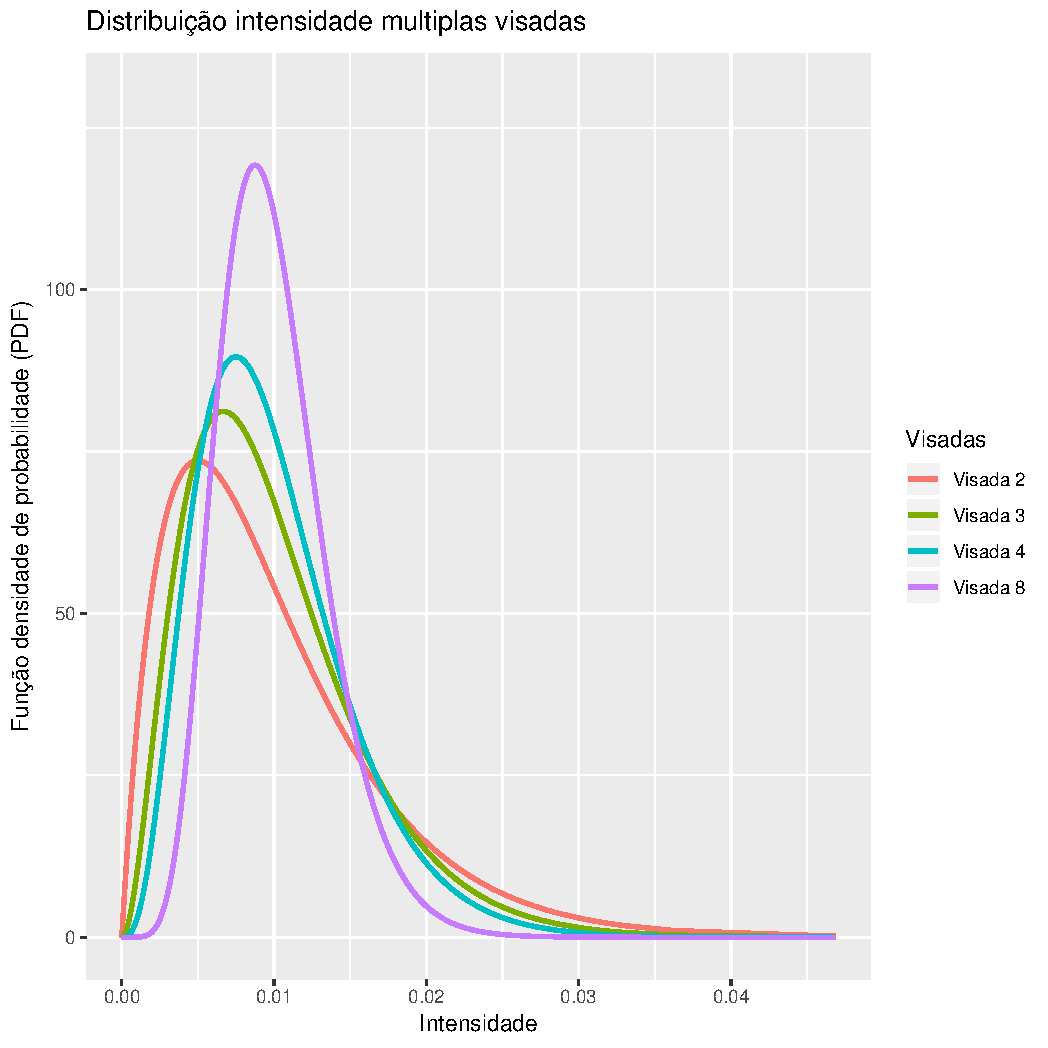
\includegraphics[width=4.0in]{dist_intensidade_multi_visadas.pdf}
	\caption{Distribuição intensidade multiplas visadas com $\sigma=0.01$.}
\label{fig2}
\end{figure}



\subsection{Função de densidade para cada canal complexo}

Sendo $(R_{ii}, R_{ij})\sim N2(0, C_{ij})$ podemos observar na tabela anterior que 
\begin{equation}
C_{ij}=\left[
\begin{array}{cc}
	\sigma_{ii}^2   &  \rho_{ii,ij}\sigma_{ii}\sigma_{ij}  \\
	\rho_{ii,ij}\sigma_{ii}\sigma_{ij} & \sigma_{ij}^2   \\
\end{array}
\right],
\end{equation}

A pdf para esta distribuição normal é:

\begin{equation}
\begin{array}{ccc}
	f_{Z_{R_{ii}R_{ij}}}(z)&=&\frac{1}{\pi\sigma_{ii}\sigma_{ij}\sqrt{1-\rho_{ii,ij}^2}}\exp\left(\frac{\rho_{ii,ij}z}{\sigma_{ii}\sigma_{ij}(1-\rho_{ii,ij})^2}\right)\\
	&&K_0\left(\frac{|z|}{\sigma_{ii}\sigma_{ij}(1-\rho_{ii,ij})^2}\right).
\end{array}
\end{equation}


Sendo $(I_{ii}, I_{ij})\sim N2(0, C_{ij})$ podemos observar na tabela anterior que 
\begin{equation}
C_{ij}=\left[
\begin{array}{cc}
	\sigma_{ii}^2   &  \rho_{ii,ij}\sigma_{ii}\sigma_{ij}  \\
	\rho_{ii,ij}\sigma_{ii}\sigma_{ij} & \sigma_{ij}^2   \\
\end{array}
\right],
\end{equation}
\begin{equation}
\begin{array}{ccc}
	f_{Z_{R_{ii}R_{ij}}}(z)&=&\frac{1}{\pi\sigma_{ii}\sigma_{ij}\sqrt{1-\rho_{ii,ij}^2}}\exp\left(\frac{\rho_{ii,ij}z}{\sigma_{ii}\sigma_{ij}(1-\rho_{ii,ij})^2}\right)\\
	&&K_0\left(\frac{|z|}{\sigma_{ii}\sigma_{ij}(1-\rho_{ii,ij})^2}\right).
\end{array}
\end{equation}

Definindo o funcional $\Theta(z;\sigma_p,\sigma_q,\gamma)$
\begin{equation}
\begin{array}{ccc}
	\Theta(z;\sigma_p,\sigma_q,\gamma)&=&\frac{1}{\pi\sigma_p\sigma_q\sqrt{1-\gamma^2}}\exp\left(\frac{\gamma z}{\sigma_p\sigma_q(1-\gamma)^2}\right)\\
	&&K_0\left(\frac{|z|}{\sigma_p\sigma_q(1-\gamma)^2}\right).
\end{array}
\end{equation}
onde,  $\sigma_p,\sigma_q,\gamma$ são  parâmetros da função.
\subsection{distribuição conjunta para  $(R_{ii}, R_{ij})\sim N2(0, C_{ij})$}
Sendo $(R_{ii}, R_{ij},I_{ii}, I_{ij})\sim N4(0, C_{ii,ij})$ podemos observar na tabela anterior que 
\begin{equation}
C_{ii,ij}=\left[
\begin{array}{cccc}
	\sigma_{ii}^2   &  \rho_{ii,ij}\sigma_{ii}\sigma_{ij} & 0&\eta_{ii,ij}\sigma_{ii}\sigma_{ij}\\
	\rho_{ii,ij}\sigma_{ii}\sigma_{ij} & \sigma_{ij}^2  & -\eta_{ii,ij}\sigma_{ii}\sigma_{ij}&0 \\
	0&-\eta_{ii,ij}\sigma_{ii}\sigma_{ij}&\sigma_{ii}^2&\rho_{ii,ij}\sigma_{ii}\sigma_{ij}\\
	\eta_{ii,ij}\sigma_{ii}\sigma_{ij}&0&\rho_{ii,ij}\sigma_{ii}\sigma_{ij}&\sigma_{ij}^2\\
\end{array}
\right],
\end{equation}
Realizar a transformação 
\begin{equation}
\left[
\begin{array}{ccc}
	 Z = R_{ii}R_{ij}+I_{ii}I_{ij} \\
	 U_1 = R_{ii}\\
	 U_2 = R_{ij}\\
	 U_3 = I_{ii}\\
\end{array}
\right],
\end{equation}

%%%%%%%%%%%%%%%%%%%%%%%%%%%%%%%%%%%%%%%%%%%%%%%%%%%%%%%%%%%%%%
De acordo com \citet{good} e \citet{lee} esta distribuição pode modelar adequadamente o comportamento estatístico de $\mathbf{s}$. A hipotêse de ser gaussiana e circular foi comprovada para dados SAR polarimétricos no artigo \citet{sarabendi}.   

A função densidade de probabilidade ({\bf pdf}) da distribuição gaussiana complexa $m$-variada é dada por
\begin{equation}\label{cap_acf_4}
    p({\bf s})=\frac{1}{\pi^m|\bf{\Sigma}_{{\bf s}}|}\exp(-{\bf s}^{H}\bf{\Sigma}_{{\bf s}}^{-1}{\bf s}), 
\end{equation}
sendo $|\cdot|$ o determinante de uma matriz ou o valor absoluto de um escalar, e $\mathbf{\Sigma}_{\bf{s}}$ é a matriz de covariância associada a $\mathbf{s}$ definida por
\begin{equation}\label{cap_acf_5}
	{\bf \Sigma_{{\bf s}}} = E[{\mathbf s}{\mathbf s}^H] = \left[
\begin{array}{cccc}
	E[S_1\overline{S_1}]  & E[{S_1}\overline{S_2}] &\hdots & E[S_1\overline{S_m}] \\
	E[S_2\overline{S_1}]  & E[{S_2}\overline{S_2}] &\hdots &E[S_2\overline{S_m}]\\
        \vdots&\vdots &\ddots &\vdots\\
	E[S_m\overline{S_1}]  & E[S_m\overline{S_2}] &\hdots &E[S_m\overline{S_m}]\\
\end{array}
\right]
\end{equation}
talque, $E[\cdot]$ denota o valor esperado e $\overline{\cdot}$ denota o conjugado complexo. A matriz de covariância é hermitiana positiva definida e contém todas as informações necessárias para caracterizar o retroespalhamento, podemos consultar mais informações em \citep{mfp}. 

Nas imagens PolSAR serão consideradas três componentes para o vetor $\mathbf{s}=[S_{hh},S_{vh},S_{vv}]^T$ e a multiplicação de $\mathbf{s}=[S_{hh},S_{vh},S_{vv}]$ pelo seu conjugado transposto $\mathbf{s}=[S_{hh},S_{vh},S_{vv}]^H$, isto é, a hermitiana do vetor, 

\begin{equation}\label{cap_acf_6}
\mathbf{s}\mathbf{s}^H = \left[
\begin{array}{c}
	S_{hh}      \\
        S_{vh}     \\
	S_{vv}      \\
\end{array}
\right]
\left[
\begin{array}{ccc}
	S_{hh}  & S_{vh}  & S_{vv}      \\
\end{array}
\right]^H = 
\left[
\begin{array}{ccc}
	S_{hh}\overline{S_{hh}} & S_{hh} \overline{S_{vh}} & S_{hh}  \overline{S_{vv}}     \\
	S_{vh} \overline{S_{hh}}  & S_{vh} \overline{S_{vh}}  & S_{vh} \overline{S_{vv}}      \\
	S_{vv} \overline{S_{hh}}  & S_{vv} \overline{S_{vh}}  & S_{vv}  \overline{S_{vv}}     \\
\end{array}
\right].
\end{equation}

A  matriz $\mathbf \Sigma_{{\mathbf s}}$ tem dimensão $3\times 3$, e pode ser definida como sendo a matriz de covariância associada a $\mathbf{s}$.
\begin{equation}\label{cap_acf_7}
\mathbf{\Sigma_{{\mathbf s}}} = E[\mathbf{s}\mathbf{s}^H] =
\left[
\begin{array}{ccc}
	E[S_{hh}\overline{S_{hh}}] & E[S_{hh} \overline{S_{vh}}] & E[S_{hh}  \overline{S_{vv}}]     \\
	E[S_{vh} \overline{S_{hh}}]  & E[S_{vh} \overline{S_{vh}}]  & E[S_{vh} \overline{S_{vv}}]      \\
	E[S_{vv} \overline{S_{hh}}]  & E[S_{vv} \overline{S_{vh}}]  & E[S_{vv}  \overline{S_{vv}}]     \\
\end{array}
\right].  
\end{equation}

Dados polarimétricos são usualmente sujeitados a um processo de várias visadas com o intuito de melhorar a razão entre o sinal e o seu ruído. Para esse fim, matrizes positivas definidas hermitianas estimadas são obtidas computando a média de $L$ visadas independentes de uma mesma cena. Resultando na matriz de covariância amostral estimada {\bf Z} conforme \citep{good, ade}
\begin{equation}\label{cap_acf_8}
\begin{array}{ccc}
    \mathbf{Z}&=&\frac{1}{L}\displaystyle{\sum_{i=1}^{L} {\mathbf{s}_i}{\mathbf{s}_i}^H}, \\
\end{array}
\end{equation}
onde $\mathbf{s}_i$ com $i = 1, \dots, L$ é uma amostra de $\mathit{L}$ vetores complexos distribuídos como $\mathbf{s}$, assim a matriz de covariância amostral associada a $\mathbf{s}_i$, com $i=1,\dots,L$ denotam o espalhamento para cada visada $L$ seguindo uma distribuição complexas de Wishart. 

Sendo agora $\mathbf{\Sigma_{s}}$ e $L$ parâmetros conhecidos a função densidade de probabilidade da distribuição Wishart por  
%
\begin{equation}\label{cap_acf_9}
    f_{\mathbf{Z}}(\mathbf{Z};\mathbf{\Sigma_{s}},L)=\frac{L^{mL}|\mathbf{Z}|^{L-m}}{|\mathbf{\Sigma_{s}}|^{L}\Gamma_m(L)} \exp(-L\traco(\mathbf{\Sigma_{s}}^{-1}\mathbf{Z})), \\
\end{equation}
onde, $\traco(\cdot)$ é o operador traço de uma matriz, $\Gamma_m(L)$ é uma função Gamma multivariada definida por
\begin{equation}\label{cap_acf_10}
	\Gamma_m(L)=\pi^{\frac{1}{2}m(m-1)} \prod_{i=0}^{m-1}\Gamma(L-i) \\
\end{equation}
e $\Gamma(\cdot)$ é a função Gamma. Podemos afirmar que $\mathbf{Z}$ é distribuído como uma distribuição Wishart denotando por $\mathbf{Z}\sim W(\mathbf{\Sigma_{s}}, L)$ e satisfazendo $E[\mathbf{Z}]=\mathbf{\Sigma_{s}}$. Sem perda de generalidade para o texto vamos usar o simbolo $\mathbf{\Sigma}$ em detrimento a $\mathbf{\Sigma_{s}}$ para representar a matriz de covariância associada a $\mathbf{s}$.

Seja a função densidade de probabilidade da distribuição complexa Wishart (\ref{cap_acf_9}) na qual vamos aplicar o logaritmo natural e suas propriedades com o intuito de reescrever a função na forma adequada para aplicar o método de estimativa de máxima verossimilhança. Assim,
\begin{equation}\label{cap_acf_11}
\begin{array}{ccc}
    \ln{f_{\mathbf{Z}}(\mathbf{Z};\mathbf{\Sigma},L)}&=&\ln{\left(\frac{L^{mL}|\mathbf{Z}|^{L-m}}{|\mathbf{\Sigma}|^{L}\Gamma_m(L)} \exp(-L\traco(\mathbf{\Sigma}^{-1}\mathbf{Z}))\right)}, \\
        \ln{\left(f_{\mathbf{Z}}(\mathbf{Z};\mathbf{\Sigma},L)\right)}&=&\ln{\left(\frac{L^{mL}|\mathbf{Z}|^{L-m}}{|\mathbf{\Sigma}|^{L}\Gamma_m(L)}\right)}+\ln{\left( \exp(-L\traco(\mathbf{\Sigma}^{-1}\mathbf{Z}))\right)}, \\
        \ln{\left(f_{\mathbf{Z}}(\mathbf{Z};\mathbf{\Sigma},L)\right)}&=&\ln{\left(L^{mL}|\mathbf{Z}|^{L-m}\right)} - \ln{\left(|\mathbf{\Sigma}|^{L}\Gamma_m(L)\right)}-L\traco(\mathbf{\Sigma}^{-1}\mathbf{Z}), \\
        \ln{\left(f_{\mathbf{Z}}(\mathbf{Z};\mathbf{\Sigma},L)\right)}&=&mL\ln{L}+(L-m)\ln{\left(|\mathbf{Z}|\right)} - \ln{\left(|\mathbf{\Sigma}|^{L}\right)}-\ln{\left(\Gamma_m(L)\right)}-L\traco(\mathbf{\Sigma}^{-1}\mathbf {Z}), \\
	\ln{\left(f_{\mathbf{Z}}(\mathbf{Z};\mathbf{\Sigma},L)\right)}&=&mL\ln{L}+L\ln{\left(|\mathbf{Z}|\right)}-m\ln{\left(|\mathbf{Z}|\right)} - L\ln{\left(|\mathbf{\Sigma}|\right)}-\ln{\left(\Gamma_m(L)\right)}-L\traco(\mathbf{\Sigma}^{-1}\mathbf{Z}), \\
\end{array}
\end{equation}
lembrando que a função Gamma multivariada é definida na equação (\ref{cap_acf_10}) então, podemos rescrever a equação da seguinte forma
\begin{equation}\label{cap_acf_12}
\begin{array}{cll}
	\ln{\left(f_{\mathbf{Z}}(\mathbf{Z};\mathbf{\Sigma},L)\right)}&=&mL\ln{L}+L\ln{\left(|\mathbf{Z}|\right)}-m\ln{\left(|\mathbf{Z}|\right)} - L\ln{\left(|\mathbf{\Sigma}|\right)}-\ln{\left(\Gamma_m(L)\right)}-L\traco(\mathbf{\Sigma}^{-1}\mathbf{Z}), \\
	\ln{\left(f_{\mathbf{Z}}(\mathbf{Z};\mathbf{\Sigma},L)\right)}&=&mL\ln{L}+L\ln{\left(|\mathbf{Z}|\right)}-m\ln{\left(|\mathbf{Z}|\right)} - L\ln{\left(|\mathbf{\Sigma}|\right)}\\
	&-&\ln{\left(\pi^{\frac{1}{2}m(m-1)} \prod_{i=0}^{m-1}\Gamma(L-i)\right)}-L\traco(\mathbf{\Sigma}^{-1}\mathbf{Z}),\\
	\ln{\left(f_{\mathbf{Z}}(\mathbf{Z};\mathbf{\Sigma},L)\right)}&=&mL\ln{L}+L\ln{\left(|\mathbf{Z}|\right)}-m\ln{\left(|\mathbf{Z}|\right)} - L\ln{\left(|\mathbf{\Sigma}|\right)}\\
        &-&\ln{\left(\pi^{\frac{1}{2}m(m-1)}\right)}-\ln{\left( \prod_{i=0}^{m-1}\Gamma(L-i)\right)}-L\traco(\mathbf{\Sigma}^{-1}\mathbf{Z}), \\
	\ln{\left(f_{\mathbf{Z}}(\mathbf{Z};\mathbf{\Sigma},L)\right)}&=&mL\ln{L}+L\ln{\left(|\mathbf{Z}|\right)}-m\ln{\left(|\mathbf{Z}|\right)} - L\ln{\left(|\mathbf{\Sigma}|\right)}\\
        &-&\frac{1}{2}m(m-1)\ln{\left(\pi\right)}-\sum_{i=0}^{m-1}\ln{\left(\Gamma(L-i)\right)}-L\traco(\mathbf{\Sigma}^{-1}\mathbf{Z}),\\
\end{array}
\end{equation}
equação equivalente pode ser encontrada em \citep{fnc2011}.


\section{Modelos para dados dados}

A matriz de espalhamento complexa {\boldmath S} é definida por
$$
\mathbf{ s} = \left[
\begin{array}{cc}
	S_{hh}   & S_{hv}   \\
	S_{vh}   & S_{vv}   \\
\end{array}
\right].
$$
% % % ACF Dizer o que significam "h" e "v"

Usaremos o caso do meio de propagação ser recíproco, isto é, $S_{hv}=S_{vh}$ tornando a matriz de espalhamento simétrica. Podemos facilitar a notação representando a matriz de espalhamento por um vetor da seguinte forma
$$
\mathbf{s} = \left[
\begin{array}{c}
	S_{vv}      \\
	S_{vh}     \\
	S_{hh}      \\
\end{array}
\right].
$$
% % % ACF Não é sempre um fato. Ocorre na maioria das vezes, e em português é "meio recíproco".

De acordo com \cite{good} a distribuição gaussiana complexa multivariada pode modelar adequadamente o comportamento estatístico de $\boldmath S$. Isto é chamado de {\it single-look complex PolSAR data representation} e podemos definir o vetor de espalhamento por $\mathbf{s}=[S_1,S_2,\dots,S_p]^T$. 
% % % ACF Acrescentei "complex"

A função densidade de probabilidade ({\boldmath pdf}) da distribuição gaussiana complexa $p-$variada é dada por
\begin{equation}\label{eqn1}
	p(\mathbf{s})=\frac{1}{\pi^p|\Sigma_{\mathbf{s}}|}\exp(-\bar{\mathbf{s}}^{T}\Sigma_{\mathbf{s}}^{-1}\mathbf{s}).
\end{equation}
O parâmetro que indexa a distribuição é a matriz de covariância, que é definida por:
\begin{equation}\label{eqn2}
	\mathbf{ \Sigma_{s}} = E[\mathbf{ss}^H] = \left[
\begin{array}{cccc}
	E(\mathbf{s_1s_1}^H)  & E(\mathbf{s_1s_2}^H) &\hdots & E({\mathbf s_1s_p}^H) \\
	E(\mathbf{ s_2s_1}^H)  & E(\mathbf {s_2 s_2}^H) &\hdots &E(\mathbf {s_2 s_p}^H)\\
        \vdots&\vdots &\ddots &\vdots\\
	E(\mathbf{ s_ps_1}^H)  & E(\mathbf {s_ps_2}^H) &\hdots &E(\mathbf {s_ps_p}^H)\\
\end{array}
\right].
\end{equation}
onde $E(\cdot)$ e $(\cdot)^H$ denotam o valor esperado e o conjugado transposto.

A matriz {\boldmath$\Sigma_{\mathbf{s}}$} é hermitiana pois se $\mathbf {S_j}= x_j+iy_j $

\begin{equation}\label{eqn3}
\begin{array}{ccc}
\mathbf{S}_j\overline{\mathbf{S}}_j&=& (x_j+iy_j)\overline{(x_j+iy_j)} \\
\mathbf{S}_j\overline{\mathbf{S}}_j&=& (x_j+iy_j)(x_j-iy_j) \\
\mathbf{S}_j\overline{\mathbf{S}}_j&=& x_j^2+y_j^2 \\
\end{array}
\end{equation}
considerando $j \neq k$
\begin{equation}\label{eqn4}
\begin{array}{ccc}
\mathbf{S}_j\overline{\mathbf{S}}_k&=& (x_j+iy_j)\overline{(x_k+iy_k)} \\
\mathbf{S}_j\overline{\mathbf{S}}_k&=& (x_j+iy_j)(x_k-iy_k) \\
\mathbf{S}_j\overline{\mathbf{S}}_k&=& (x_jx_k+y_jy_k)+i(x_ky_j-x_jy_k) \\
\end{array}
\end{equation}
ainda,
\begin{equation}\label{eqn5}
\begin{array}{ccc}
	\overline{\mathbf{S}_k\overline{\mathbf{S}}}_j&=&\overline{ (x_k+iy_k)\overline{(x_j+iy_j)} }\\
	\overline{\mathbf{S}_k\overline{\mathbf{S}}}_j&=&\overline{ (x_k+iy_k)(x_j-iy_j)} \\
	\overline{\mathbf{S}_k\overline{\mathbf{S}}}_j&=&\overline{ (x_kx_j+y_ky_j)+i(x_jy_k-x_ky_j) }\\
	\overline{\mathbf{S}_k\overline{\mathbf{S}}}_j&=&(x_kx_j+y_ky_j)-i(x_jy_k-x_ky_j) \\
	\overline{\mathbf{S}_k\overline{\mathbf{S}}}_j&=&(x_kx_j+y_ky_j)+i(x_ky_j-x_jy_k) \\
\end{array}
\end{equation}
Portanto1
\begin{equation}\label{eqn6}
\begin{array}{ccc}
	\mathbf{S}_j\overline{\mathbf{S}}_j&=&\overline{\mathbf{S}_j\overline{\mathbf {S}}}_j \\
	\mathbf{S}_j\overline{\mathbf{S}}_k&=&\overline{\mathbf{S}_k\overline{\mathbf {S}}}_j \\
\end{array}
\end{equation}
Assim com $j$ e $k$ varrendo toda a matriz podemos afirmar que $\mathbf{\Sigma_{\mathbf{s}}}=\mathbf{\Sigma_{ s}}^H$ portanto hermitiana.


Dados polarimétricos são usualmente sujeitados a um processo {\it multilook} com o intuito de melhorar a razão sinal-ruído.
% % % ACF "relação senhal-ruído"
Para esse fim, matrizes positivas definidas hermitianas são obtidas computando a médias de $L$ visadas 
% % % ACF "visadas", mas ninguém usa
independentes de uma mesma cena. Isto resulta na matriz de covariância {\boldmath{Z}} dada por:
\begin{equation}\label{eqn7}
	\mathbf{Z}=\frac{1}{L}\sum_{i=1}^{L} \mathbf{s_is_i}^H .
\end{equation}
% % % ACF Código LaTeX simplificado

\subsubsection{Coeficiente de correlação {\it Multilook}}

O coeficiente de correlação complexo é um importante parâmetro para descrever a função de densidade de probabilidade. 
Podemos defini-lo como
\begin{equation}\label{eqn8}
	\rho_c=\frac{E[\mathbf{s_is_j}^H]}{\sqrt{E[|\mathbf{s_i}|^2]E[|\mathbf{s_j}|^2]}} =|\rho_c|e^{i\theta}.
\end{equation}
% % % ACF Não complique LaTeX
em que {\boldmath $s_i$} e {\boldmath $s_j$} 
% % % ACF Repare que o negrito matemático se faz de outra maneira
são duas componentes da matriz de espalhamento ou dois retorno do radar polarimétrico ou interferométrico SAR. 
Para dados de radar polarimétricos representado pela matriz de Mueller, $\rho_c$ pode ser calculado encontrando a média da vizinhança de um pixel de uma matriz Mueller. A magnitude de $\rho_c$ pode também ser estimada usando duas intensidade  {\it multilook} $Z_{ii}$ e $Z_{jj}$. O coeficiente de correlação de dados $L$ looks intensidade é definida como   
% % % ACF Eram L looks, agora são n. Unificar a notação
\begin{equation}\label{eqn9}
	\rho_I^{(n)}=\frac{E[(Z_{ii}-\overline{Z_{ii}})(Z_{jj}-\overline{Z_{jj}})]}{\sqrt{E[(Z_{ii}-\overline{Z_{ii}})^2][(Z_{jj}-\overline{Z_{jj}})^2]}}. \\
\end{equation}

No apêndice do artigo \cite{lee} foi mostrado que 

\begin{equation}\label{eqn10}
	\rho_I^{(n)}= |\rho_c|^2\\
\end{equation}

Sendo 

\begin{equation}\label{eqn11}
\begin{array}{ccc}
	\mathbf{S_i}&=&a_{R}+ia_{I} \\
        \mathbf{S_j}&=&b_{R}+ib_{I} \\
\end{array}
\end{equation}

Assim a equação (\ref{eqn8}) pode ser reescrita

\begin{equation}\label{eqn12}
\begin{array}{ccc}
	\rho_c&=&\frac{E[(a_{R}+ia_{I})\overline{(b_{R}+ib_{I})}]}{\sqrt{E[a_{R}^2+a_{I}^2]E[b_{R}^2+b_{I}^2]}}. \\
	\rho_c&=&\frac{E[(a_{R}+ia_{I})(b_{R}-ib_{I})]}{\sqrt{E[a_{R}^2+a_{I}^2]E[b_{R}^2+b_{I}^2]}}. \\
	\rho_c&=&\frac{E[a_{R}b_{R}+ia_{I}b_{R}-ia_{R}b_{I}+a_{I}b_{I}]}{\sqrt{E[a_{R}^2+a_{I}^2]}\sqrt{E[b_{R}^2+b_{I}^2]}}. \\
	\rho_c&=&\frac{E[a_{R}b_{R}+ia_{I}b_{R}-ia_{R}b_{I}+a_{I}b_{I}]}{\sqrt{E[a_{R}^2+a_{I}^2]}\sqrt{E[b_{R}^2+b_{I}^2]}}. \\
\end{array}
\end{equation}
Definindo os desvios padrões,
\begin{equation}\label{eqn13}
\begin{array}{ccc}
	\sigma_{a}	&=&\sqrt{E[a_{R}^2+a_{I}^2]} \\
	\sigma_{b}      &=&\sqrt{E[b_{R}^2+b_{I}^2]} \\
\end{array}
\end{equation}

\begin{equation}\label{eqn14}
\begin{array}{ccc}
	\rho_c&=&\frac{E[a_{R}b_{R}+ia_{I}b_{R}-ia_{R}b_{I}+a_{I}b_{I}]}{\sigma_a\sigma_b}. \\
	\rho_c&=&\frac{E[a_{R}b_{R}+a_{I}b_{I}+i(a_{I}b_{R}-a_{R}b_{I})]}{\sigma_a\sigma_b}. \\
	\rho_c&=&\frac{E[a_{R}b_{R}]+E[a_{I}b_{I}]+i(E[a_{I}b_{R}]-E[a_{R}b_{I})]}{\sigma_a\sigma_b}. \\
	\rho_c&=&\frac{E[a_{R}b_{R}]}{\sigma_a\sigma_b}+\frac{E[a_{I}b_{I}]}{\sigma_a\sigma_b}+i\left(\frac{E[a_{I}b_{R}]}{\sigma_a\sigma_b}-\frac{E[a_{R}b_{I}]}{\sigma_a\sigma_b}\right). \\
\end{array}
\end{equation}
Definindo
\begin{equation}\label{eqn15}
\begin{array}{ccccccccc}
	\rho_{RR}=\frac{E[a_{R}b_{R}]}{\sigma_a\sigma_b},&&\rho_{II}=\frac{E[a_{I}b_{I}]}{\sigma_a\sigma_b},&&\rho_{IR}=\frac{E[a_{I}b_{R}]}{\sigma_a\sigma_b},&&\rho_{RI}=\frac{E[a_{R}b_{I}]}{\sigma_a\sigma_b}. \\
\end{array}
\end{equation}

Portanto, 
\begin{equation}\label{eqn16}
	\rho_c=\frac{(\rho_{RR}+\rho_{II})+i(\rho_{IR}-\rho_{RI})}{2}. \\
\end{equation}

\textcolor{red}{obs:Explicar melhor o fator 2}

Devido a condição de ser gaussiana circular

\begin{equation}\label{eqn17}
	\rho_{RR}=\rho_{II},\quad \rho_{IR}=-\rho_{RI}. \\
\end{equation}
podemos escrever $\rho_c$
\begin{equation}\label{eqn18}
	\rho_c=\rho_{RR}+i\rho_{IR}. \\
\end{equation}

Portanto

\begin{equation}\label{eqn19}
	|\rho_c|^2=\rho_{RR}^2+\rho_{IR}^2. \\
\end{equation}

O processo de {\bf Multilook} produz
\begin{equation}\label{eqn20}
\begin{array}{ccc}
	A_n&=&\frac{1}{n}\sum_{k=1}^{n} [a_{R}^2(k)+a_{I}^2(k)]. \\
	B_n&=&\frac{1}{n}\sum_{k=1}^{n} [b_{R}^2(k)+b_{I}^2(k)]. \\
\end{array}
\end{equation}

Assumindo a independência estatística entre amostras, a média e o desvio padrão podem ser definidos por
\begin{equation}\label{eqn21}
\begin{array}{cccccccccccc}
	\overline{A_n}&=&E[A_n]&=&2E[a_{R}^2(k)]&=&2\sigma_a^2,&SD[A_n]&=&\frac{2\sigma_a^2}{\sqrt{n}}.\\
	\overline{B_n}&=&E[B_n]&=&2E[b_{R}^2(k)]&=&2\sigma_b^2,&SD[B_n]&=&\frac{2\sigma_b^2}{\sqrt{n}}.\\
\end{array}
\end{equation}

O coeficiente de correlação {\it Multilook} para intensidade (equação (\ref{eqn9})) pode ser escrito por:

\begin{equation}\label{eqn22}
	\rho_I^{(n)}=\frac{E[(A_n-\overline{A_n})(B_n-\overline{B_n})]}{SD[A_n]SD[B_n]}. \\
	%\rho_I^{(n)}&=&\frac{E[(A_nB_n-A_n\overline{B_n}-\overline{A_n}B_n+\overline{A_n}\overline{B_n}]}{SD[A_n]SD[B_n]}. \\
	%\rho_I^{(n)}&=&\frac{E[(A_nB_n]-E[A_n\overline{B_n}]-E[\overline{A_n}B_n]+E[\overline{A_n}\overline{B_n}]}{SD[A_n]SD[B_n]}. \\
	%\rho_I^{(n)}&=&\frac{E[(A_nB_n]-E[A_n\overline{B_n}]-E[\overline{A_n}B_n]+E[\overline{A_n}\overline{B_n}]}{SD[A_n]SD[B_n]}. \\
\end{equation}

Assumindo a independência entre as amostras e depois de algumas manipulações algébricas para o numerador da equação (\ref{eqn22}). 
\begin{equation}\label{eqn23}
	E[(A_n-\overline{A_n})(B_n-\overline{B_n})]=\frac{1}{n^2}\sum_{k=1}^{n}[E[(a_{R}^2(k)+a_{I}^2(k))(b_{R}^2(k)+b_{I}^2(k))]-4\sigma_a^2\sigma_b^2] \\
\end{equation}
\textcolor{red}{OBS: Entender melhor a equação (\ref{eqn23}) e (\ref{eqn24})}.
\begin{equation}\label{eqn24}
	E[(A_n-\overline{A_n})(B_n-\overline{B_n})]=\frac{4}{n}\sigma_a^2\sigma_b^2|\rho_c|^2\\
\end{equation}

Agora substituindo em (\ref{eqn22})

\begin{equation}\label{eqn25}
\begin{array}{ccc}
	\rho_I^{(n)}&=&\frac{\frac{4}{n}\sigma_a^2\sigma_b^2|\rho_c|^2}{SD[A_n]SD[B_n]}. \\
	\rho_I^{(n)}&=&\frac{\frac{4}{n}\sigma_a^2\sigma_b^2|\rho_c|^2}{\frac{2\sigma_a^2}{\sqrt{n}}\frac{2\sigma_b^2}{\sqrt{n}}}. \\
\end{array}
\end{equation}

completando as simplificaçãoes

\begin{equation}\label{eqn26}
	\rho_I^{(n)}=|\rho_c|^2. \\
\end{equation}

\textcolor{blue}{OBS: Esta relação mostra que o coeficiente de correlação da intensidade não depende dos {\it nlooks}.}



\subsubsection{Distribuição conjunta do {\it Multilook} $|S_i|^2$ e $|S_j|^2$ }

O $PDF$ conjunto retorna de dois canais correlacionados dos radares polarimétricos e interferométricos são importantes. As $PDF's$ conjuntas conduzem a derivação da intensidade e amplitude razão $PDF's$. Da equação (\ref{eqn42}) temos que as intensidades {\it multilook} sejam 

\begin{equation}\label{eqn59}
\begin{array}{ccccc}
	R_1&=&\frac{1}{n}\sum_{k=1}^{n}|S_i(k)|^2&=&\frac{B_1C_{11}}{n}\\
	R_2&=&\frac{1}{n}\sum_{k=1}^{n}|S_j(k)|^2&=&\frac{B_2C_{22}}{n}\\
\end{array}
\end{equation}

Integrando a equação (\ref{eqn52}) em relação a $\eta$ e $\psi$. A $PDF$ é

\begin{equation}\label{eqn60}
	p(B_1,B_2)=\frac{\left(B_1B_2\right)^{\frac{n-1}{2}}\exp\left(-\frac{B_1+B_2}{1-|\rho_c|^2}\right)}{\Gamma(n)(1-|\rho_c|^2)|\rho_c|^{n-1}}I_{n-1}\left(2\sqrt{B_1B_2}\frac{|\rho_c|}{1-|\rho_c|^2}\right)
\end{equation}

Sendo
\begin{equation}\label{eqn61}
	I_{\mu}(Z)=\frac{(\frac{z}{2})^{\mu}}{\Gamma(\mu+1)} F_{1}^{0}[-;\mu+1;\frac{z^2}{4}]
\end{equation}

\textcolor{red}{OBS: As integrações na equação (\ref{eqn52}) não foram realizadas neste estudo.}
\begin{equation}\label{eqn62}
	p(B_1,B_2)=\frac{n^{n+1}\left(R_1R_2\right)^{\frac{n-1}{2}}\exp\left(-\frac{n(\frac{R_1}{C_{11}}+\frac{R_2}{C_{22}})}{1-|\rho_c|^2}\right)}{(C_{11}C_{22})^{\frac{n+1}{2}}\Gamma(n)(1-|\rho_c|^2)|\rho_c|^{n-1}}I_{n-1}\left(2n\sqrt{\frac{R_1R_2}{C_{11}C_{22}}}\frac{|\rho_c|}{1-|\rho_c|^2}\right)
\end{equation}

\textcolor{red}{OBS: Verificar o surgimento de um fator $\frac{n^2}{C_{11}C_{22}}$ na equação  (\ref{eqn62}) - Mudança de variável!!!!!.}

\subsubsection{Distribuição razão intensidade e amplitude para {\it multilook}}

A razão de intensidade e amplitude entre $S_{hh}$ e $S_{vv}$ são importantes no estudo de radares polarimétricos. A $PDF's$ razão de intensidade e amplitude normalizada será mostrada agora

\begin{equation}\label{eqn63}
\begin{array}{ccccccc}
	\mu&=&\frac{B_1}{B_2}&=&\frac{\sum_{k=1}^{n}\frac{|S_i(k)|^2}{C_{11}}}{\sum_{k=1}^{n}\frac{|S_j(k)|^2}{C_{22}}}&=&\frac{\sum_{k=1}^{n}|S_i(k)|^2}{\tau\sum_{k=1}^{n}|S_j(k)|^2}\\
\end{array}
\end{equation}

Onde $\tau=\frac{C_{11}}{C_{22}}$.

A $PDF$ razão intensidade {\it multlook} normalizada é mostrada no apêndice $(C)$ do artigo \cite{lee}  


\begin{equation}\label{eqn64}
	p^{(n)}(\mu)=\frac{\Gamma(2n)(1-|\rho_c|^2)^{n}(1+\mu)\mu^{n-1}}{\Gamma(n)\Gamma(n)\left[(1+\mu)^2-4|\rho_c|^2\mu \right]^{\frac{2n+1}{2}}}\\
\end{equation}

\textcolor{red}{OBS: Não realizei as contas do apêndice $(C)$.}

Realizando a troca de variável $\nu=\sqrt{\mu}$ a equação (\ref{eqn64}) pode ser rescrita por
\begin{equation}\label{eqn65}
	p^{(n)}(\nu)=\frac{2\Gamma(2n)(1-|\rho_c|^2)^{n}(1+\nu^2)\nu^{2n-1}}{\Gamma(n)\Gamma(n)\left[(1+\nu^2)^2-4|\rho_c|^2\nu^2 \right]^{\frac{2n+1}{2}}}\\
\end{equation}
As $PDF's$ razão de intensidade e amplitude entre os {\it multilook} $\mathbf{S_1}$ e $\mathbf{S_2}$ podem ser facilmente deduzidas das seguintes definições e posterior aplicação nas equações (\ref{eqn64}) e (\ref{eqn65}). definindo 
\begin{equation}\label{eqn66}
\begin{array}{ccccc}
	w&=&\frac{\sum_{k=1}^{n}|S_i(k)|^2}{\sum_{k=1}^{n}|S_i(k)|^2}&=&\tau\mu\\
	z&=&\sqrt{w}&=&\sqrt{\tau}\nu
\end{array}
\end{equation}
Portanto a distribuição da razão $w$ de intensidade {\it multilook} é
\begin{equation}\label{eqn67}
	p^{(n)}(w)=\frac{\tau^{n}\Gamma(2n)(1-|\rho_c|^2)^{n}(\tau+w)w^{n-1}}{\Gamma(n)\Gamma(n)\left[(\tau+w)^2-4\tau|\rho_c|^2w \right]^{\frac{2n+1}{2}}}.
\end{equation}
Portanto a distribuição da razão $z$ de amplitude {\it multilook} é
\begin{equation}\label{eqn68}
	p^{(n)}(z)=\frac{\tau^{n}\Gamma(2n)(1-|\rho_c|^2)^{n}(\tau+z^2)z^{2n-1}}{\Gamma(n)\Gamma(n)\left[(\tau+z^2)^2-4\tau|\rho_c|^2z^2 \right]^{\frac{2n+1}{2}}}.
\end{equation}

A discusão será limitada para estatística da razão $\nu$ amplitude normalizada. A figura (\ref{fig2}) mostra a distribuição razão amplitude apresentada na equação  (\ref{eqn65}). Notadamente a medida que $n$ aumenta tendemos a ter uma aproximação da "função" delta de Dirac e uma concentração em torno da abscissa $\nu=1$.

\textcolor{blue}{OBS: Processos de {\it multilook} reduzem a variância.}


\section{Método da máxima verossimilhança aplicado nas funções densidades de probabilidades}

\subsection{Método da verossimilhança aplicado na pdf univariada $\Gamma$.}
Considerando a função distribuição de densidade univariada gaussiana 
\begin{equation}\label{pdf_gauss_univ}
	f_{Z}(z;\mu,L)=\frac{L^{L}}{\Gamma(L)\mu^{L}} z^{L-1}\exp\left\{-L\frac{z}{\mu}\right\}, \\
\end{equation}
onde, $\mu>0$ e $L>0$. Aplicando o logaritmo natural na equação~\eqref{pdf_gauss_univ}  e realizando algumas manipulações algébricas teremos:
\begin{equation}\nonumber
\begin{array}{ccl}
	\ln f_{Z}(z;\mu,L)&=&\ln \left(\frac{L^{L}}{\Gamma(L)\mu^{L}} z^{L-1}\exp\left\{-L\frac{z}{\mu}\right\}\right), \\
	                                         &=&\ln\left(\frac{L}{\mu}\right)^L-\ln\Gamma(L)+ \ln z^{L-1} + \ln \exp\left\{-L\frac{z}{\mu}\right\}, \\
%	                                         &=&L\ln\frac{L}{\mu}-\ln\Gamma(L)+(L-1)\ln z - \frac{L}{\mu} z,\\	                                         
\end{array}
\end{equation}
resultanto na função,
\begin{equation}\label{func_log_univ_gaussiana}
	\ln f_{Z}(z;\mu,L)=L\ln\frac{L}{\mu}-\ln\Gamma(L)+(L-1)\ln z - \frac{L}{\mu} z.
\end{equation}

A função log-verossimilhança pode ser deduzida da seguinte maneira, dado a amostra $\bm z = (z_1,\dots,z_n)$, 
\begin{equation}\nonumber
\begin{split}
  \ell(\bm z;\mu, L)=\ln\prod_{k=1}^{n}f_Z(z_k;\mu,L)\\
  \ell(\bm z;\mu, L)=\sum_{k=1}^{n}\ln f_Z(z_k;\mu,L),
 \end{split}
 \end{equation}
usando a funçcão~\eqref{func_log_univ_gaussiana} teremos,
\begin{equation}\nonumber
\begin{split}
    \ell(\bm z;\mu, L)&=\sum_{k=1}^{n}\ln f_Z(z_k;\mu,L)\\
                      &=\sum_{k=1}^{n}\left[L\ln\frac{L}{\mu}-\ln\Gamma(L)+(L-1)\ln z_k - \frac{L}{\mu} z_k\right]\\
                      &=\sum_{k=1}^{n}L\ln\frac{L}{\mu}-\sum_{k=1}^{n}\ln\Gamma(L)+(L-1)\sum_{k=1}^{n}\ln z_k - \frac{L}{\mu}\sum_{k=1}^{n} z_k\\
                      &=L\ln\frac{L}{\mu}\sum_{k=1}^{n}1-\ln\Gamma(L)\sum_{k=1}^{n}1+(L-1)\sum_{k=1}^{n}\ln z_k - \frac{L}{\mu}\sum_{k=1}^{n} z_k\\
                      &=L\ln\frac{L}{\mu}n-\ln\Gamma(L)n+(L-1)\sum_{k=1}^{n}\ln z_k - \frac{L}{\mu}\sum_{k=1}^{n} z_k.\\                
 \end{split}
 \end{equation}

Definimos a equação log-verossimilhança para a PDF univariada~(\ref{func_log_univ_gaussiana}).
\begin{equation}\nonumber
    \ell(\bm z;\mu, L)=n\left[L\ln\frac{L}{\mu}-\ln\Gamma(L)\right]+(L-1)\sum_{k=1}^{n}\ln z_k - \frac{L}{\mu}\sum_{k=1}^{n} z_k,\\                
 \end{equation}
e a forma reduzida, 
\begin{equation}
\ell(\bm z;\mu, L) = 
n \left[L\ln \frac{L}{\mu} - \ln \Gamma(L)\right]
+L \sum_{k=1}^{n}\ln z_k -\frac{L}{\mu}\sum_{k=1}^{n} z_k.
\label{eq:LogLikelihoodGamma_red}
\end{equation}


Vamos obter $(\widehat L, \widehat \mu)$, o estimador de máxima verossimilhança (MLE) de $(L, \mu)$ baseado $\bm z$, por maximizar~\eqref{eq:LogLikelihoodGamma_red} com o método BFGS implementado no pacote \texttt{maxLik}~\citep{ht}. Vamos preferir otimização resolvendo $\nabla\ell=\bm 0$ com intuito de melhorar a estabilidade numérica.

O função é a log-verossimilhança reduzida para as amostras internas e externas da faixa de dados denotadas respectivamento como $\bm z_\text{I}$ e $\bm z_\text{E}$. Cada faixa de dados $\bm z = (z_1,z_2,\dots,z_n)$ é particionada em duas amostras disjuntas na posição $j$:  
$$
\bm z = (\underbrace{z_1,z_2,\dots,z_j}_{\bm z_\text{I}}, 
\underbrace{z_{j+1}, z_{j+2},\dots,z_n}_{\bm z_\text{E}}).
$$
Vamos assumir dois diferentes modelos para cada partição:
$\bm Z_\text{I} \sim \Gamma(\mu_\text{I},L_\text{I})$, e
$\bm Z_\text{E} \sim \Gamma(\mu_\text{E},L_\text{E})$.
Vamos estimar $(\mu_\text{I},L_\text{I})$ e $(\mu_\text{E},L_\text{E})$ com $\bm z_\text{I}$ e $\bm z_\text{E}$, respectivamente, maximizando~\eqref{eq:LogLikelihoodGamma_red}, e obtendo $(\widehat{\mu}_\text{I}, \widehat{L}_\text{I})$ e $(\widehat{\mu}_\text{E}, \widehat{L}_\text{E})$.


A log-verossimilhança no ponto $j$ é, então
\begin{equation}\label{eq:TotalLogLikelihood}
\begin{split}
%\ell(j&;\bm z_\text{I},\bm z_\text{E}) = \\
\ell(j&;\widehat{\mu}_I, \widehat{L}_I,\widehat{\mu}_E, \widehat{L}_E)=\\
&j \big[\widehat{L}_\text{I}\ln (\widehat{L}_\text{I} / \widehat{\mu}_\text{I}) - \ln \Gamma(\widehat{L}_\text{I})\big]
+\widehat{L}_\text{I} \sum_{k=1}^{j}\ln z_k -\frac{\widehat{L}_\text{I}}{\widehat{\mu}_\text{I}}\sum_{k=1}^{j} z_k +\\
&(n-j) \big[\widehat{L}_\text{E}\ln (\widehat{L}_\text{E} / \widehat{\mu}_\text{E}) - \ln \Gamma(\widehat{L}_\text{E})\big]
+\widehat{L}_\text{E} \sum_{k=j+1}^{n}\ln z_k - \frac{\widehat{L}_\text{E}}{\widehat{\mu}_\text{E}}\sum_{k=j+1}^{n} z_k.
\raisetag{2.2em}
\end{split}
\end{equation}
Vamos aplicar o método GenSA para encontrar
$$
\widehat{\jmath}= \arg\max\limits_{j\in [\min_s,N-\min_s]}\ell(j;\widehat{\mu}_I, \widehat{L}_I,\widehat{\mu}_E, \widehat{L}_E),
$$ 
onde $\min_s$ é o tamanho mínimo da amostra definido por $14$.

Desta maneira, vamos obter uma estimativa para a borda em cada canal de intensidade.
Note que esse método pode ser estendido e/ou modificado para lidar com qualquer tipo de dados.



\subsubsection*{Aplicação em imagem simulada}

O método da máxima verossimilhança \eqref{eq:TotalLogLikelihood} foi aplicado na imagem simulada com duas amostras, e as evidências de bordas estão mostradas na figura. \textcolor{red}{Base de dados gamf}
 \begin{figure*}[hbt]
	\centering
     \subfloat[Evidências no canal $\text{hh}$ \label{evidencias_hh_hv_vv_gamf:a}]{%
       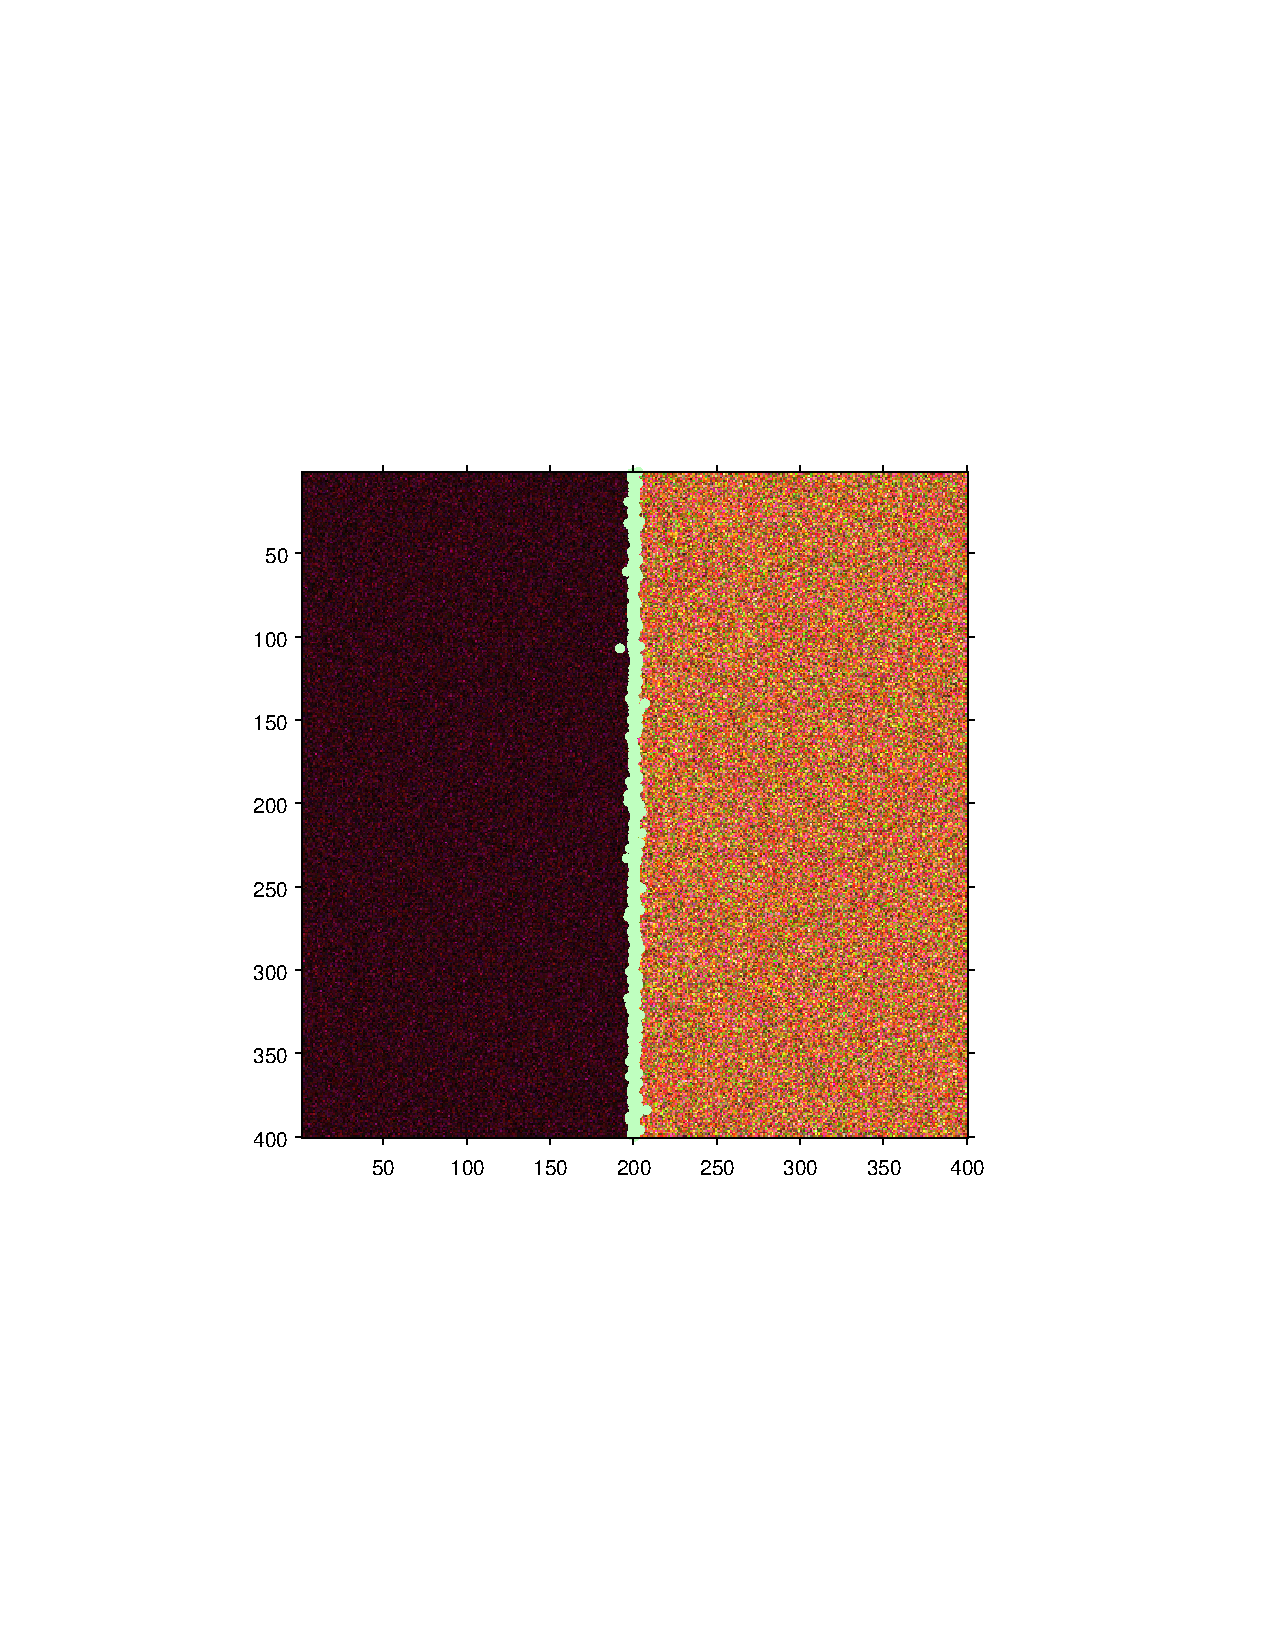
\includegraphics[width=0.5\linewidth]{im_sim_gamf_hh_evid_param_L_mu_14_pixel}
     }
     \subfloat[Evidências no canal $\text{hv}$ \label{evidencias_hh_hv_vv_gamf:b}]{%
       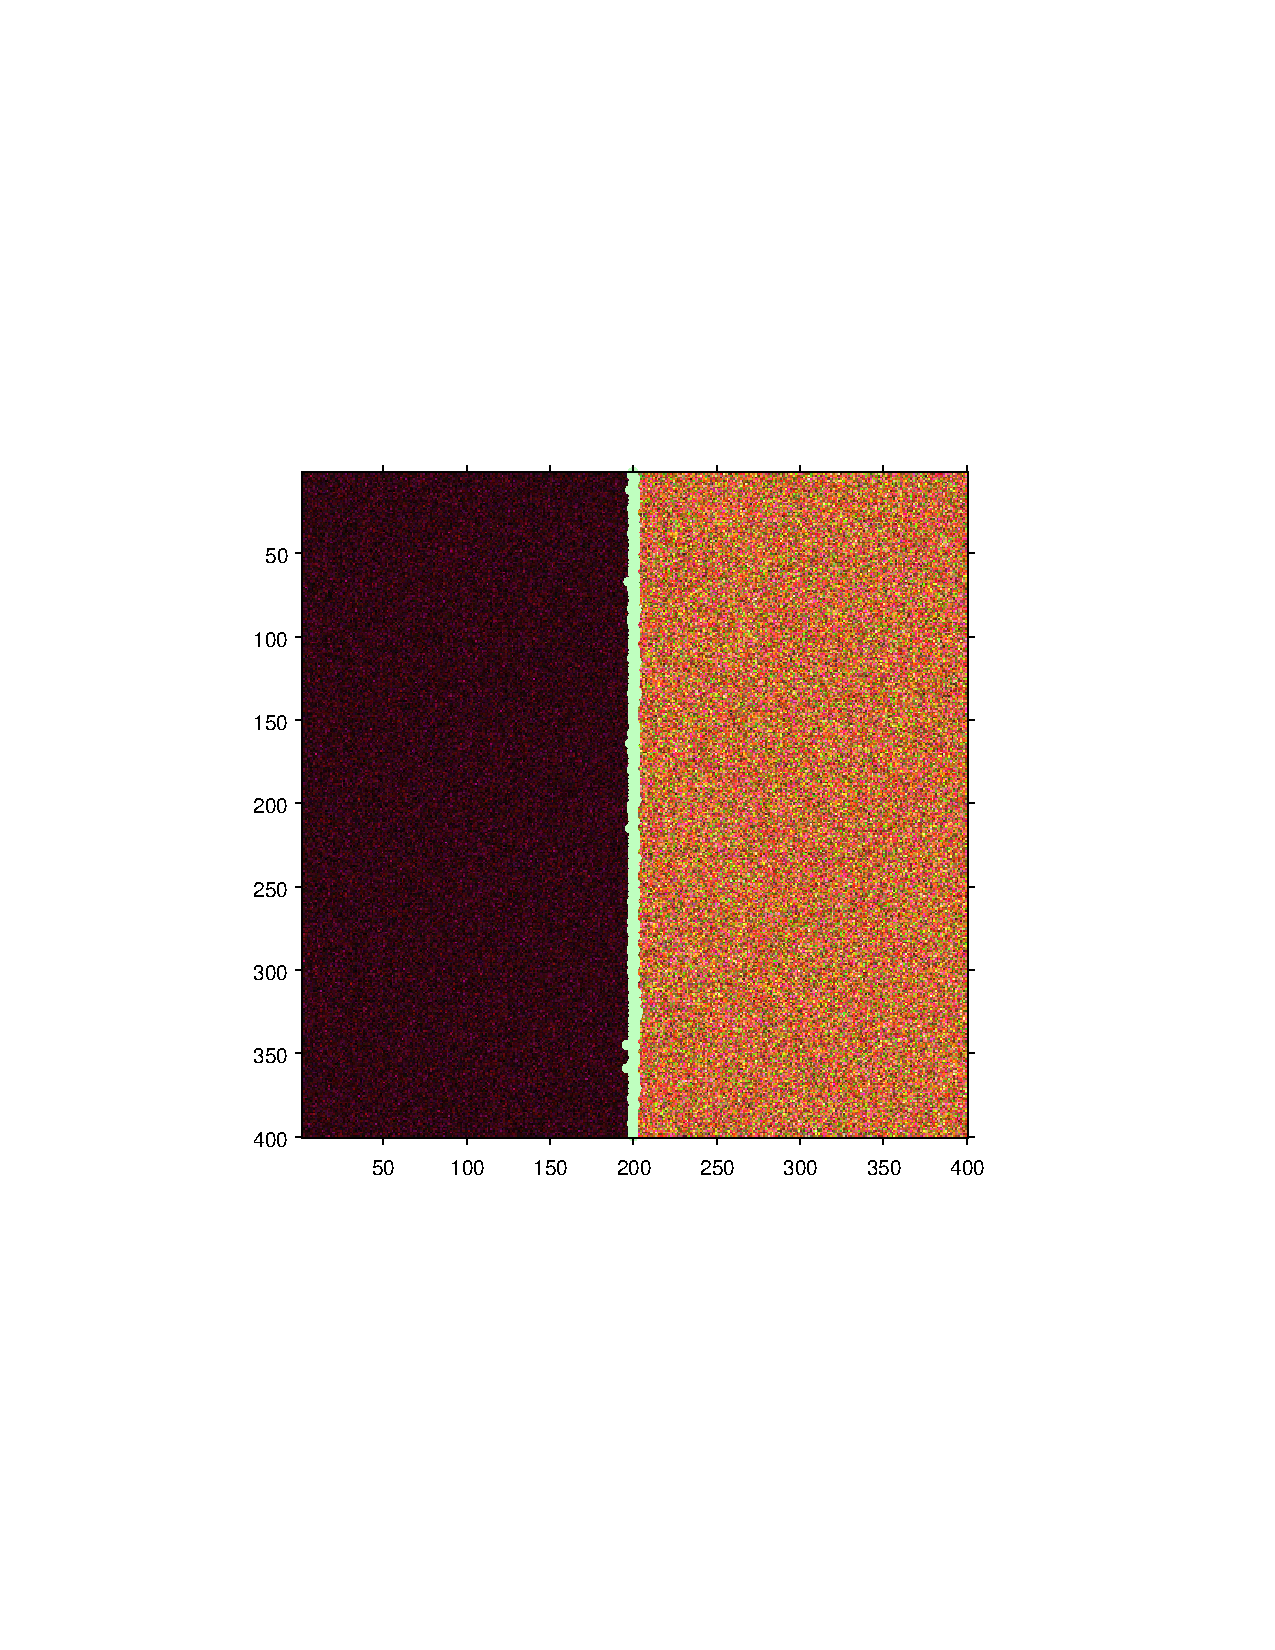
\includegraphics[width=0.5\linewidth]{im_sim_gamf_hv_evid_param_L_mu_14_pixel}
     }      
   %  \subfloat[Evidências no canal $\text{vv}$ \label{evidencias_hh_hv_vv_gamf:c}]{%
    %   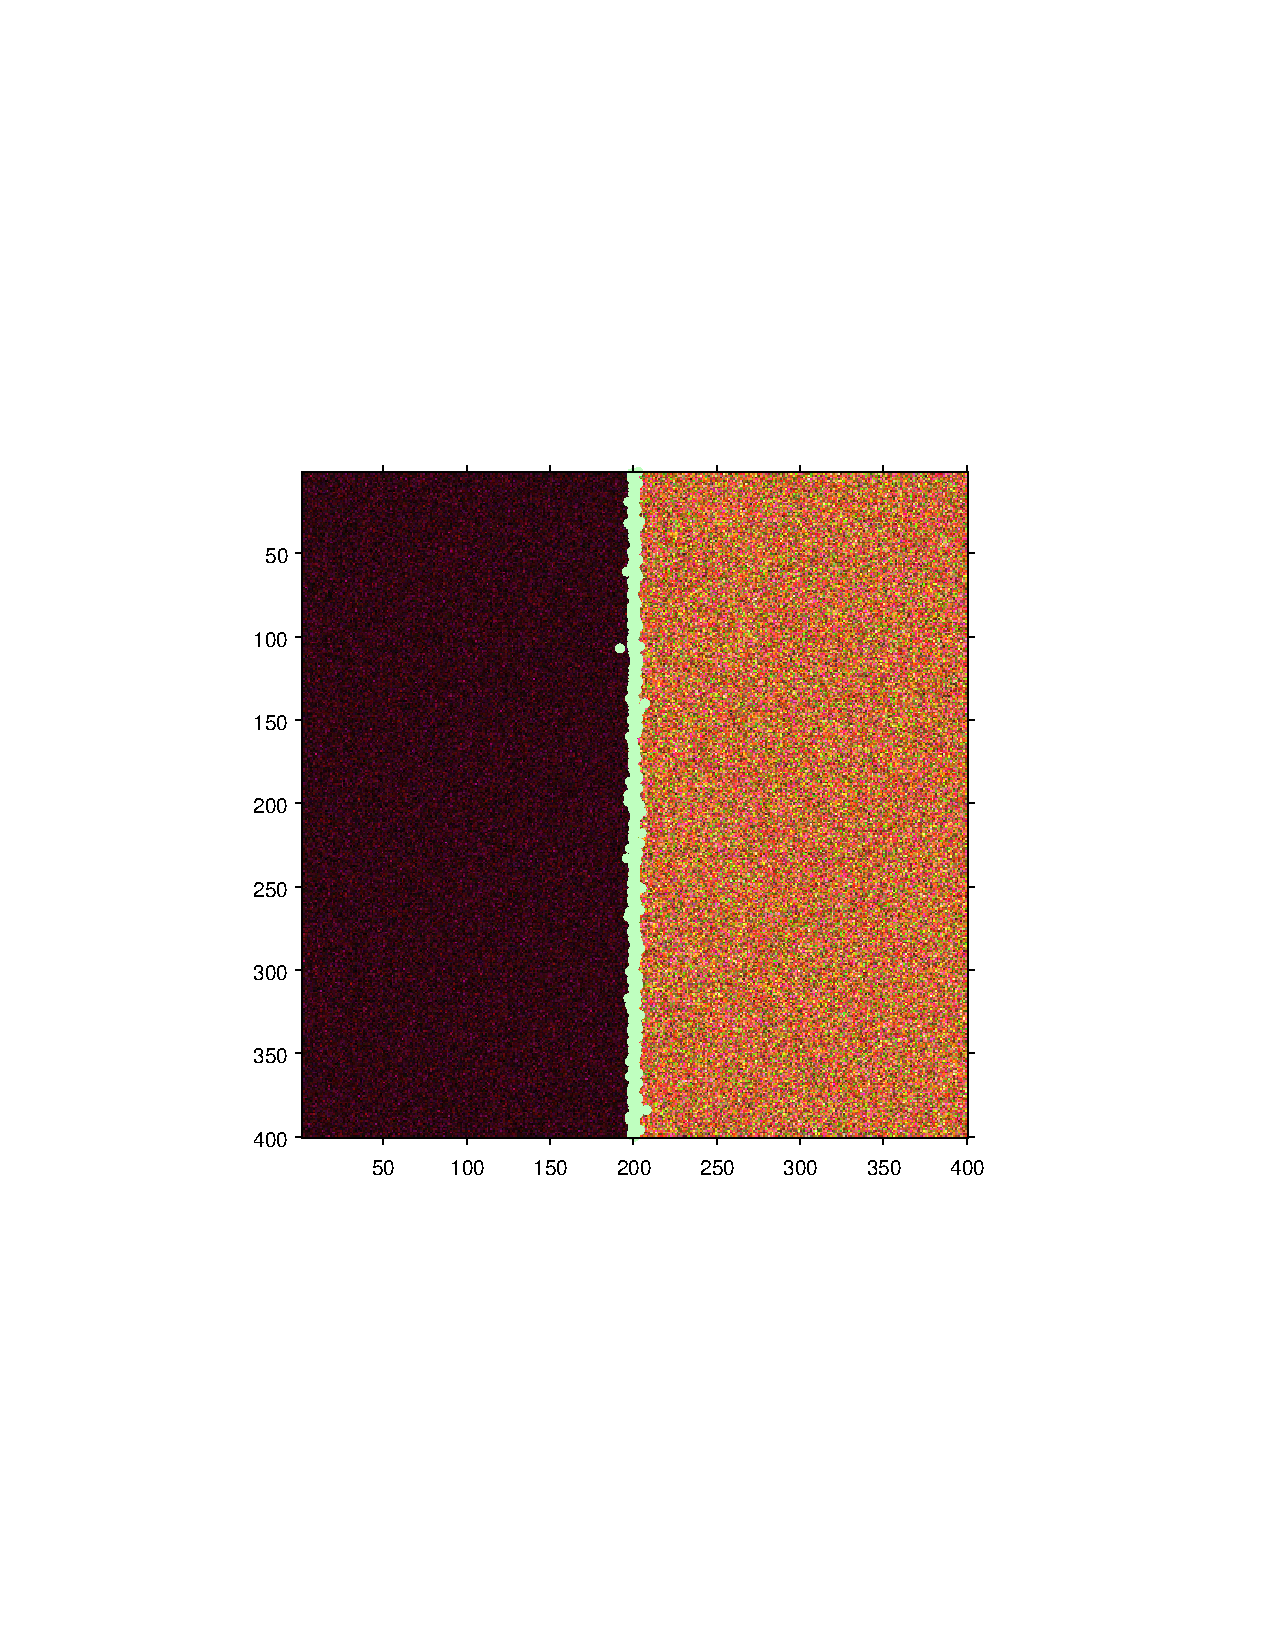
\includegraphics[width=0.5\linewidth]{im_sim_gamf_hh_evid_param_L_mu_14_pixel}
    % }
    \caption{Evidências de bordas para os três canais de intensidade}
     \label{evidencias_hh_hv_vv_gamf} 
   \end{figure*}
   
   \begin{figure*}[hbt]
	\centering
     \subfloat[Evidências no canal $\text{vv}$ \label{evidencias_hh_hv_vv_gamf:c}]{%
       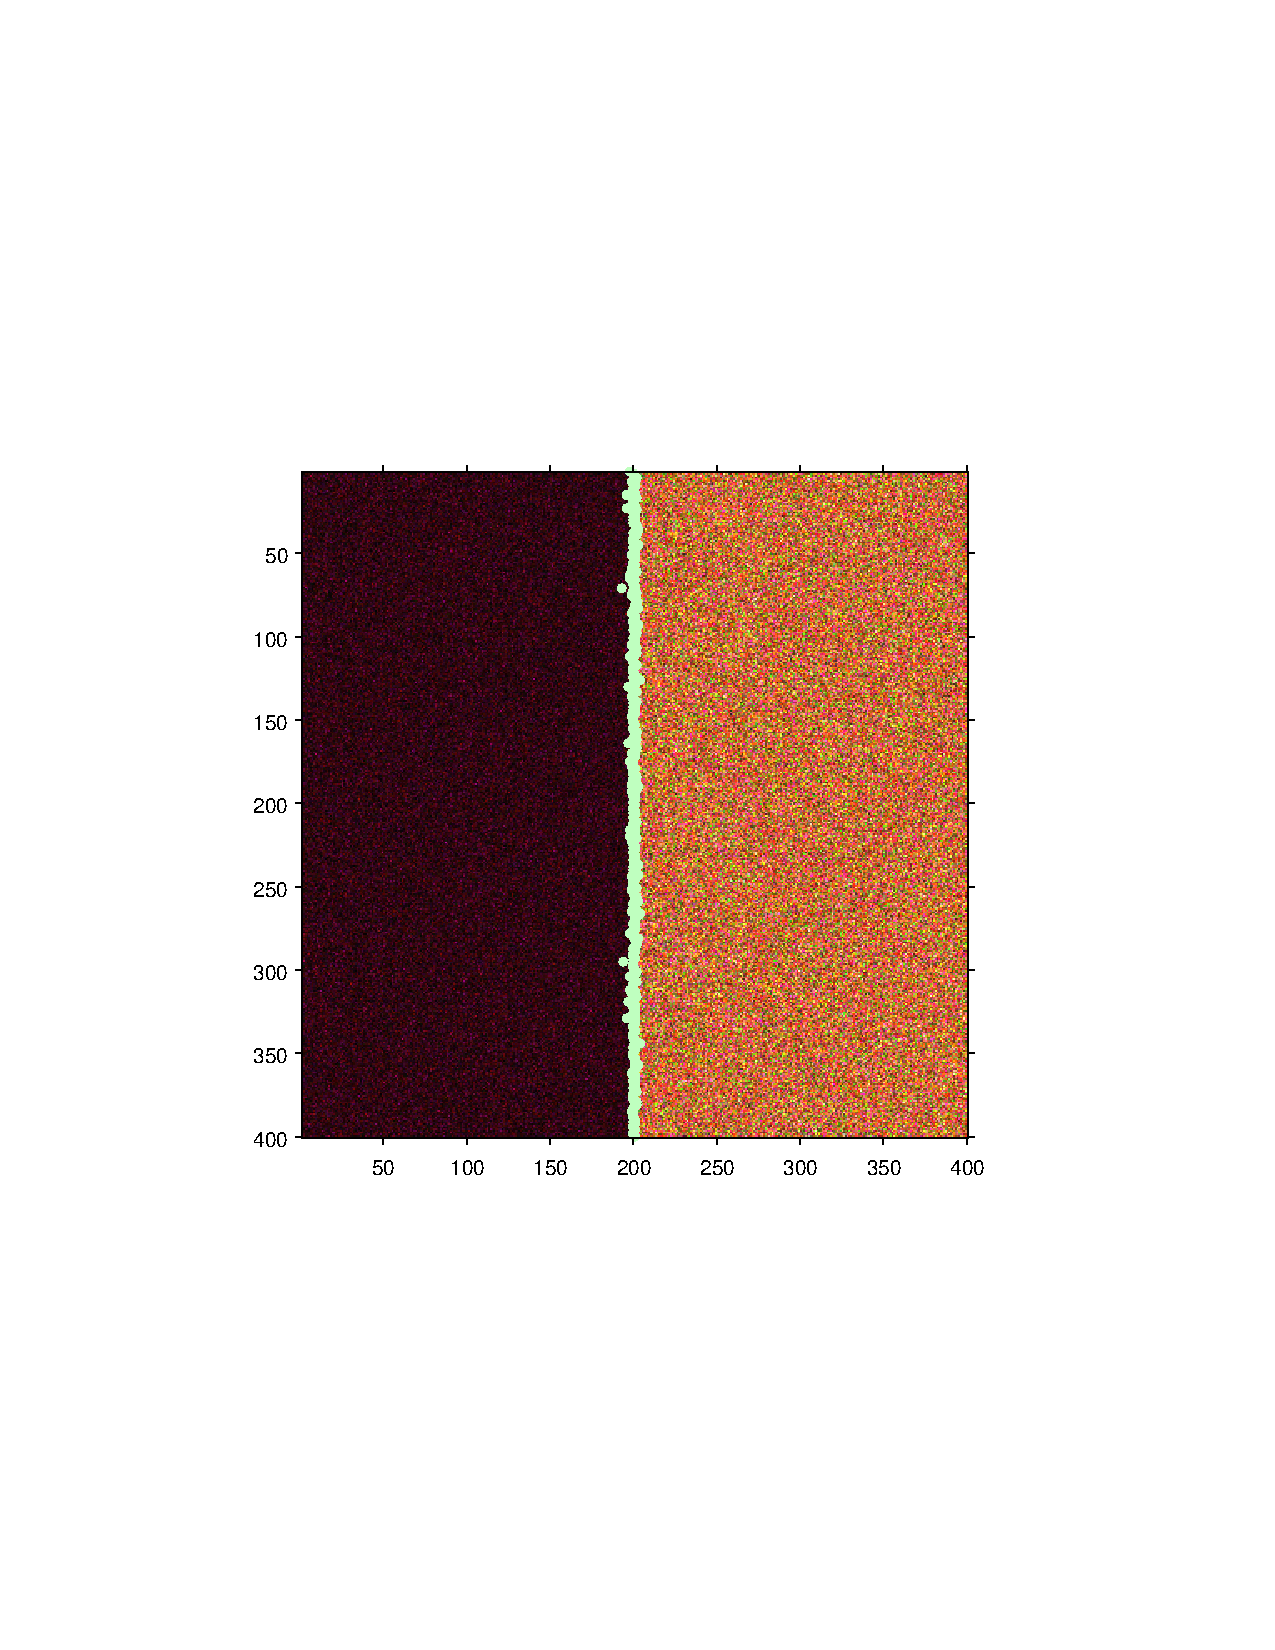
\includegraphics[width=0.5\linewidth]{im_sim_gamf_vv_evid_param_L_mu_14_pixel}
     }
    \caption{Evidências de bordas para os três canais de intensidade}
     \label{evidencias_hh_hv_vv_gamf} 
   \end{figure*}

\subsection{Método da verossimilhança aplicado na PDF univariada magnitude do produto}
%\subsection{Função de densidade para a magnitude do produto $\mathbf{S}_i$ e $\mathbf{S}_j$}
A magnitude do produto $\mathbf{S}_i$ e $\mathbf{S}_j$ é uma importante medida para as imagem SAR polarimétrica, definimos a magnitude normalizada por 
\begin{equation}
	\bm\xi = \frac{\left|\frac{1}{L} \sum_{k=1}^L\mathbf{S}_i(k)\mathbf{S}_j^H(k) \right|}{\sqrt{E[|\mathbf{S}_i|^2]E[|\mathbf{S}_i|^2]}}=\frac{g}{h}.
\end{equation}
onde é definido por $g=|\mathbf{S}_i\mathbf{S}_j^H|$ e $h=\sqrt{E[|\mathbf{S}_i|^2]E[|\mathbf{S}_i|^2]}$.

A  função densidade de probabilidade univariada para $\xi$ é obtida da integração da equação \eqref{ap:eq_pdf_aux} com respeito a $B_1$, $B_2$ e $\psi$ é
\begin{equation}\label{eq:pdf_mag_prod}
\begin{array}{lcl}
	f(\bm \xi;\rho, L)&=&\frac{4L^{L+1}\bm\xi^L}{\Gamma(L)(1-|\rho|^2)}I_0\left(\frac{2|\rho|L\bm\xi}{1-|\rho|^2}\right)K_{L-1}\left(\frac{2L\bm\xi}{1-|\rho|^2}\right),
		\end{array}
\end{equation}
onde $I_0$ e $K_{L-1}$ são funções de Bessel modificadas,e onde, $\rho>0$ e $L>0$.


A figura \eqref{fig:pdf_mag_prod} mostra a função densidade magnitude do produto com a variação das visadas $L=2,3,4$, e $8$, 
\begin{figure}[hbt]
\centering
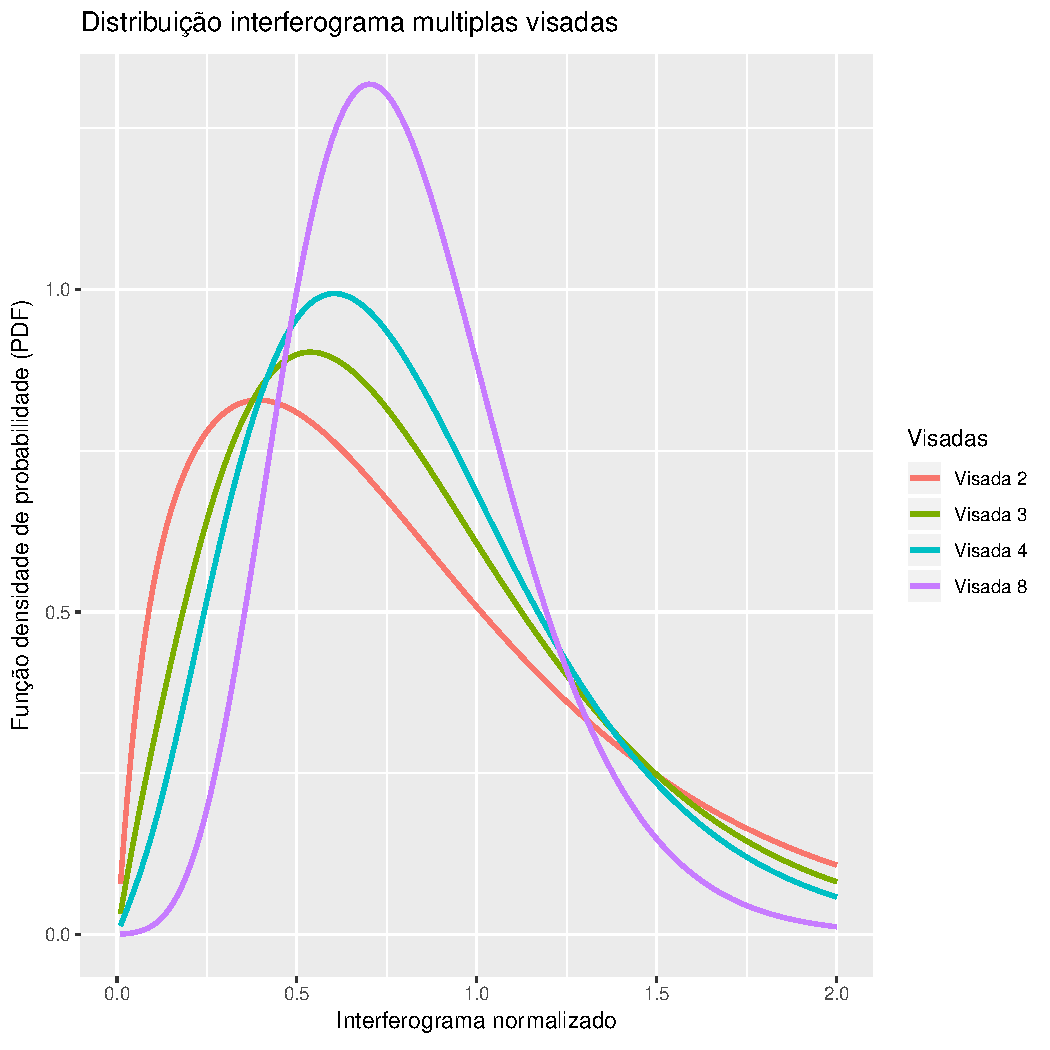
\includegraphics[width=4.0in]{dist_interferograma_multi_visadas.pdf}
	\caption{Distribuição magnitude do produto múltiplas visadas.}
\label{fig:pdf_mag_prod}
\end{figure}


O logaritmo natural é aplicado na equação~\eqref{eq:pdf_mag_prod} com o objetivo de construir o método de máxima verossimilhança, realizando algumas manipulações algébricas, teremos
\begin{equation}\nonumber
\begin{split}
	\ln f(\bm\xi;\rho,L)&=\ln\left(\frac{4L^{L+1}\bm\xi^L}{\Gamma(L)(1-|\rho|^2)}I_0\left(\frac{2|\rho|L\bm\xi}{1-|\rho|^2}\right)K_{L-1}\left(\frac{2L\bm\xi}{1-|\rho|^2}\right)\right),\\
	&=\ln\left(\frac{4L^{L+1}\bm\xi^L}{\Gamma(L)(1-|\rho|^2)}\right)+\ln I_0\left(\frac{2|\rho|L\bm\xi}{1-|\rho|^2}\right)+ \ln K_{L-1}\left(\frac{2L\bm\xi}{1-|\rho|^2}\right),\\
	&=\ln (4L^{L+1}\bm\xi^L)-\ln(\Gamma(L)(1-|\rho|^2))+\ln I_0\left(\frac{2|\rho|L\bm\xi}{1-|\rho|^2}\right)+ \ln K_{L-1}\left(\frac{2L\bm\xi}{1-|\rho|^2}\right),\\
     &=\ln (4)+\ln L^{L+1}+\ln \bm\xi^L-\ln\Gamma(L)-\ln(1-|\rho|^2)\\
     &+\ln I_0\left(\frac{2|\rho|L\bm\xi}{1-|\rho|^2}\right)+ \ln K_{L-1}\left(\frac{2L\bm\xi}{1-|\rho|^2}\right),\\
	&=\ln (4)+(L+1)\ln L+L\ln \bm\xi-\ln\Gamma(L)-\ln(1-|\rho|^2)\\
	&+\ln I_0\left(\frac{2|\rho|L\bm\xi}{1-|\rho|^2}\right)+ \ln K_{L-1}\left(\frac{2L\bm\xi}{1-|\rho|^2}\right).
		\end{split}
\end{equation}

Encontramos a função logarítmica para a \textbf{PDF} univariada magnitude do produto
\begin{equation}\label{eq:log_vero_mag_produto}
\begin{split}
	\ln f(\bm\xi; \rho,\L)&=\ln (4)+(L+1)\ln L+L\ln \bm\xi-\ln\Gamma(L)-\ln(1-|\rho|^2)\\
	                      &+\ln I_0\left(\frac{2|\rho|L\bm\xi}{1-|\rho|^2}\right)+ \ln K_{L-1}\left(\frac{2L\bm\xi}{1-|\rho|^2}\right).
	\end{split}
\end{equation}

A função log-verossimilhança pode ser deduzida da seguinte maneira, dado a amostra $\bm\xi = (\xi_1,\dots,\xi_n)$, 
\begin{equation}\nonumber
\begin{split}
  \ell(\bm \xi;\rho, L)=\ln\prod_{k=1}^{n}f(\xi_k;\rho,L)\\
  \ell(\bm \xi;\rho, L)=\sum_{k=1}^{n}\ln f(\xi_k;\rho,L),
 \end{split}
 \end{equation}
usando a função~\eqref{eq:log_vero_mag_produto} teremos,
\begin{equation}\nonumber
\begin{split}
    \ell(\bm \xi;\rho, L)&=\sum_{k=1}^{n}\ln f(\xi_k;\rho,L)\\
                         &=\sum_{k=1}^{n}\left[\ln (4)+(L+1)\ln L+L\ln \xi_k-\ln\Gamma(L)-\ln(1-|\rho|^2)\right.\\
                         &\left.+\ln I_0\left(\frac{2|\rho|L\xi_k}{1-|\rho|^2}\right)+ \ln K_{L-1}\left(\frac{2L\xi_k}{1-|\rho|^2}\right)\right],\\
	 \end{split}
 \end{equation}
 
 \begin{equation}\nonumber
\begin{split}
    \ell(\bm \xi;\rho, L)&=\ln (4)\sum_{k=1}^{n}1+(L+1)\ln L\sum_{k=1}^{n}1+L\sum_{k=1}^{n}\ln \xi_k-\ln\Gamma(L)\sum_{k=1}^{n}1-\ln(1-|\rho|^2)\sum_{k=1}^{n}1\\
                         &+\sum_{k=1}^{n}\ln I_0\left(\frac{2|\rho|L\xi_k}{1-|\rho|^2}\right)+ \sum_{k=1}^{n}\ln K_{L-1}\left(\frac{2L\xi_k}{1-|\rho|^2}\right)\\
                         &=n\ln (4)+n(L+1)\ln L+L\sum_{k=1}^{n} \ln\xi_k-n\ln\Gamma(L)-n\ln(1-|\rho|^2)\\
                         &+\sum_{k=1}^{n}\ln I_0\left(\frac{2|\rho|L\xi_k}{1-|\rho|^2}\right)+ \sum_{k=1}^{n}\ln K_{L-1}\left(\frac{2L\xi_k}{1-|\rho|^2}\right)\\
                         &=n\left[\ln (4)+(L+1)\ln L-\ln\Gamma(L)-\ln(1-|\rho|^2)\right]+L\sum_{k=1}^{n} \ln\xi_k\\
                         &+\sum_{k=1}^{n}\ln I_0\left(\frac{2|\rho|L\xi_k}{1-|\rho|^2}\right)+ \sum_{k=1}^{n}\ln K_{L-1}\left(\frac{2L\xi_k}{1-|\rho|^2}\right).\\
\end{split}
 \end{equation}
 
Definimos a equação log-verossimilhança para a PDF univariada~(\ref{eq:pdf_mag_prod}).
\begin{equation}\nonumber
\begin{split}
    \ell(\bm\xi;\rho, L)&=n\left[\ln (4)+(L+1)\ln L-\ln\Gamma(L)-\ln(1-|\rho|^2)\right]+L\sum_{k=1}^{n} \ln\xi_k\\
                         &+\sum_{k=1}^{n}\ln I_0\left(\frac{2|\rho|L\xi_k}{1-|\rho|^2}\right)+ \sum_{k=1}^{n}\ln K_{L-1}\left(\frac{2L\xi_k}{1-|\rho|^2}\right),\\
\end{split}
 \end{equation}
e a forma reduzida,
\begin{equation}\label{eq:eq_log_vero_mag_prod_red}
\begin{split}
    \ell(\bm \xi;\rho, L)&=n\left[(L+1)\ln L-\ln\Gamma(L)-\ln(1-|\rho|^2)\right]+L\sum_{k=1}^{n} \ln\xi_k\\
                         &+\sum_{k=1}^{n}\ln I_0\left(\frac{2|\rho|L\xi_k}{1-|\rho|^2}\right)+ \sum_{k=1}^{n}\ln K_{L-1}\left(\frac{2L\xi_k}{1-|\rho|^2}\right).\\
\end{split}
 \end{equation} 



As figuras \eqref{fig:prod_mag_l_50_r_35} até \eqref{fig:prod_mag_l_350_r_35} mostram a função de log-verossimilhança da pdf magnitude de produtos \eqref{eq:eq_log_vero_mag_prod_red} aplicada para a amostra de duas folhas simulada. No processo fixamos arbitrariamente a linha 35 da amostra e variamos o número de pixel entre 50, 150, 250 e 250. Desta maneira construímos duas funções $\ell{j}$, uma para cada lado da amostra.
 \begin{figure*}[hbt]
	\centering
     \subfloat[Pixel variando de 1 até 50 na linha 35.  \label{fig:prod_mag_l_rho_1_50}]{%
       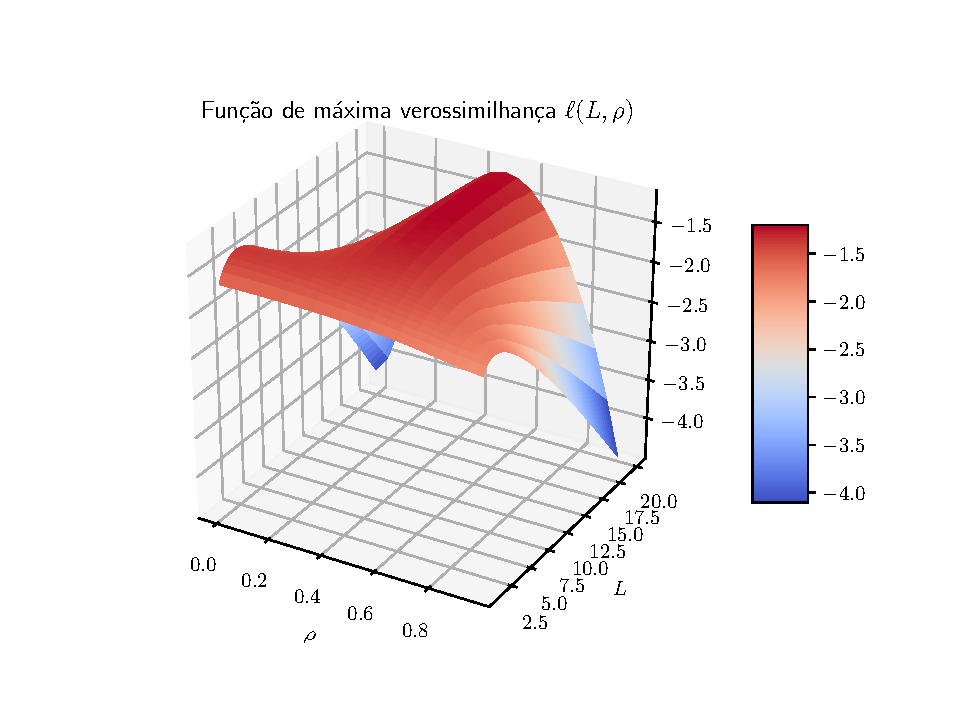
\includegraphics[width=0.50\linewidth]{fig_pdf_mag_prod_r_35_1_to_50}
     }
     \subfloat[Pixel variando de 51 até 400 na linha 35. \label{fig:prod_mag_l_rho_51_400}]{%
       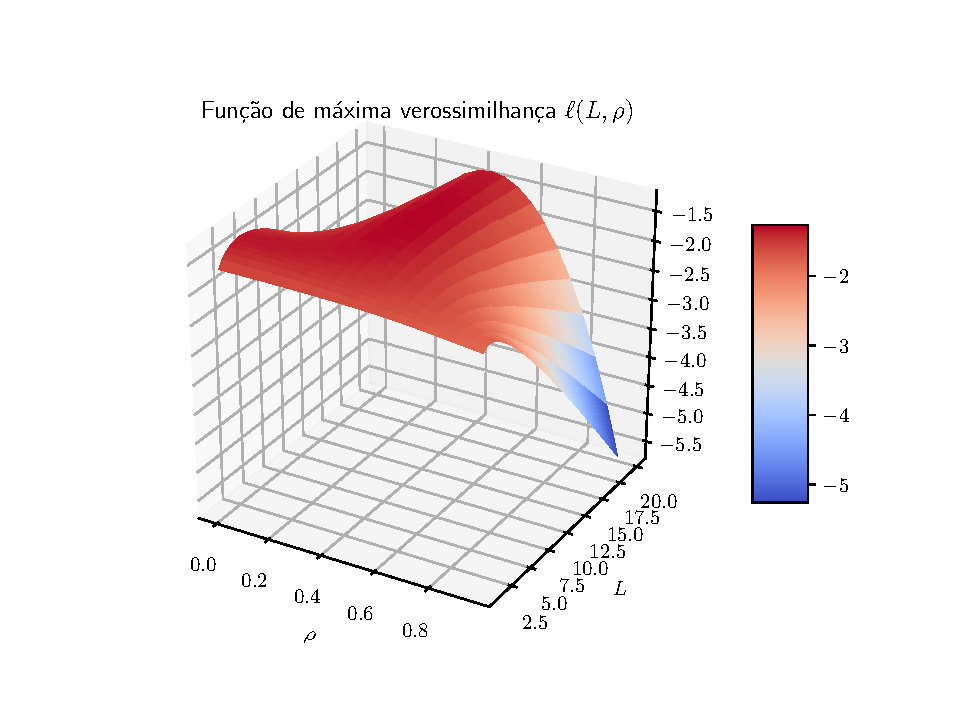
\includegraphics[width=0.50\linewidth]{fig_pdf_mag_prod_r_35_51_to_400}
     }
     \caption{Funções de máxima verossimilhança produto de magnitude com pixel fixo 50.}
     \label{fig:prod_mag_l_50_r_35} 
   \end{figure*}
   
   \begin{figure*}[hbt]
	\centering
     \subfloat[Pixel variando de 1 até 150 na linha 35.  \label{fig:prod_mag_l_rho_1_150}]{%
       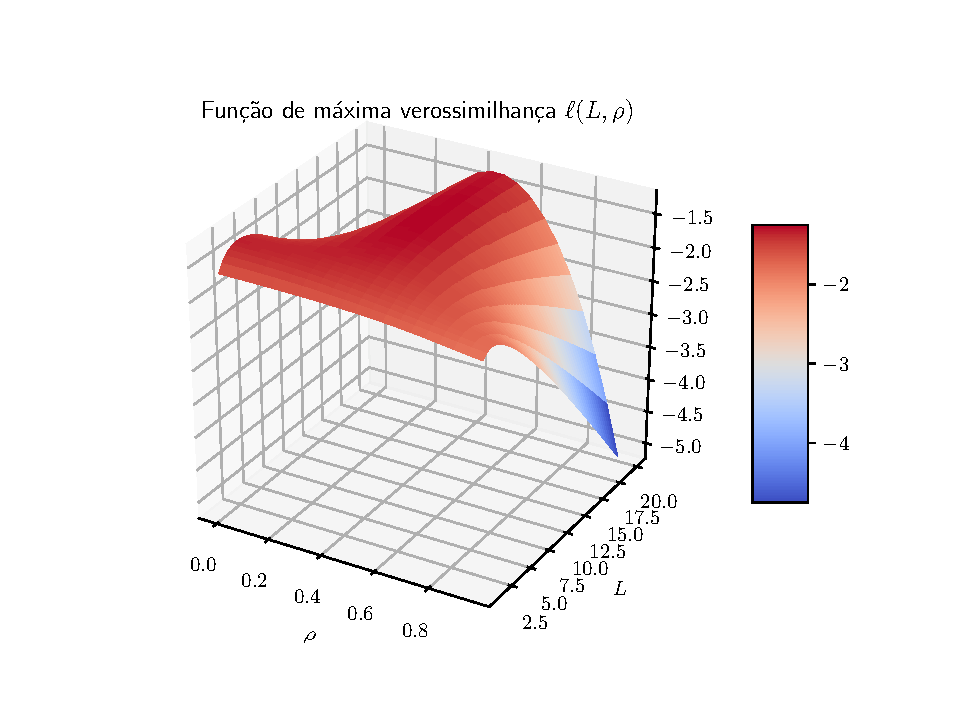
\includegraphics[width=0.50\linewidth]{fig_pdf_mag_prod_r_35_1_to_150}
     }
     \subfloat[Pixel variando de 151 até 400 na linha 35. \label{fig:prod_mag_l_rho_151_400}]{%
       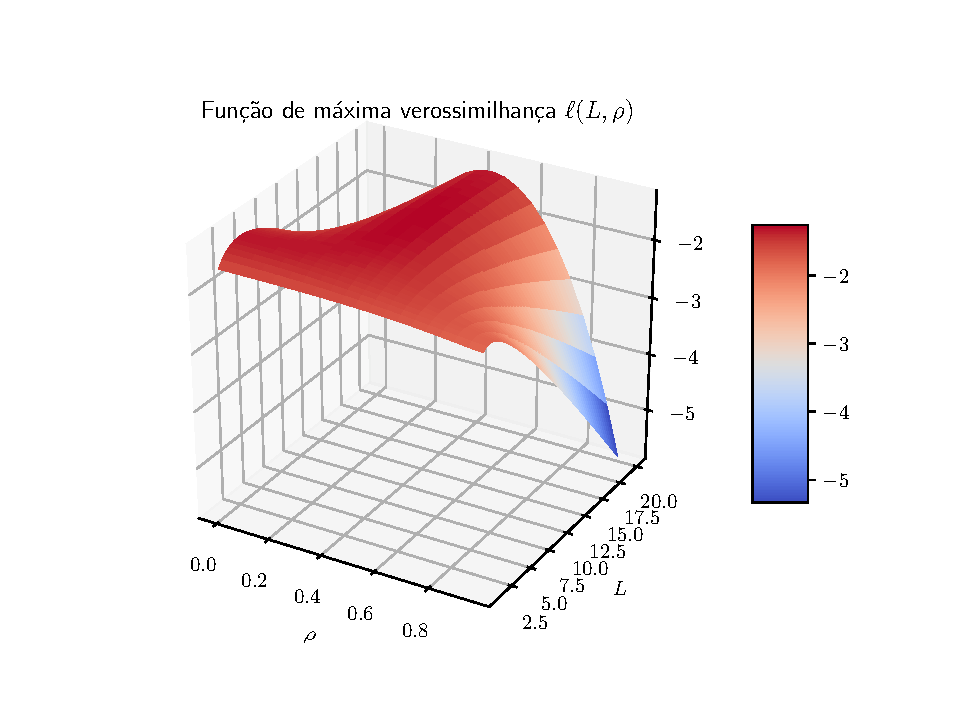
\includegraphics[width=0.50\linewidth]{fig_pdf_mag_prod_r_35_151_to_400}
     }
     \caption{Funções de máxima verossimilhança produto de magnitude com pixel fixo 150.}
     \label{fig:prod_mag_l_150_r_35} 
   \end{figure*}

\begin{figure*}[hbt]
	\centering
     \subfloat[Pixel variando de 1 até 250 na linha 35.  \label{fig:prod_mag_l_rho_1_250}]{%
       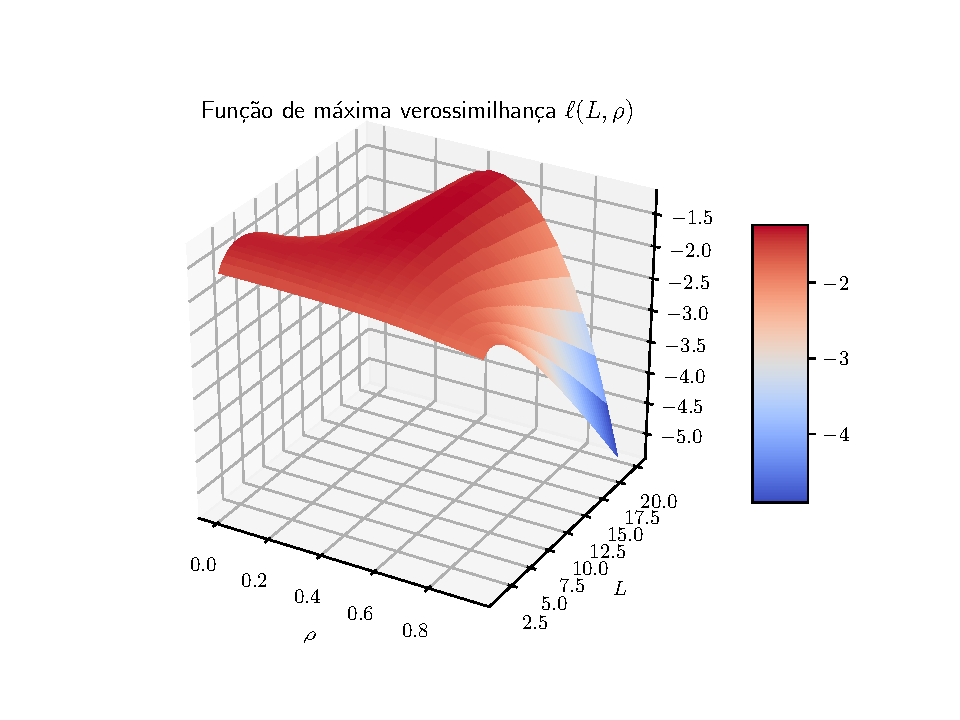
\includegraphics[width=0.50\linewidth]{fig_pdf_mag_prod_r_35_1_to_250}
     }
     \subfloat[Pixel variando de 251 até 400 na linha 35. \label{fig:prod_mag_l_rho_251_400}]{%
       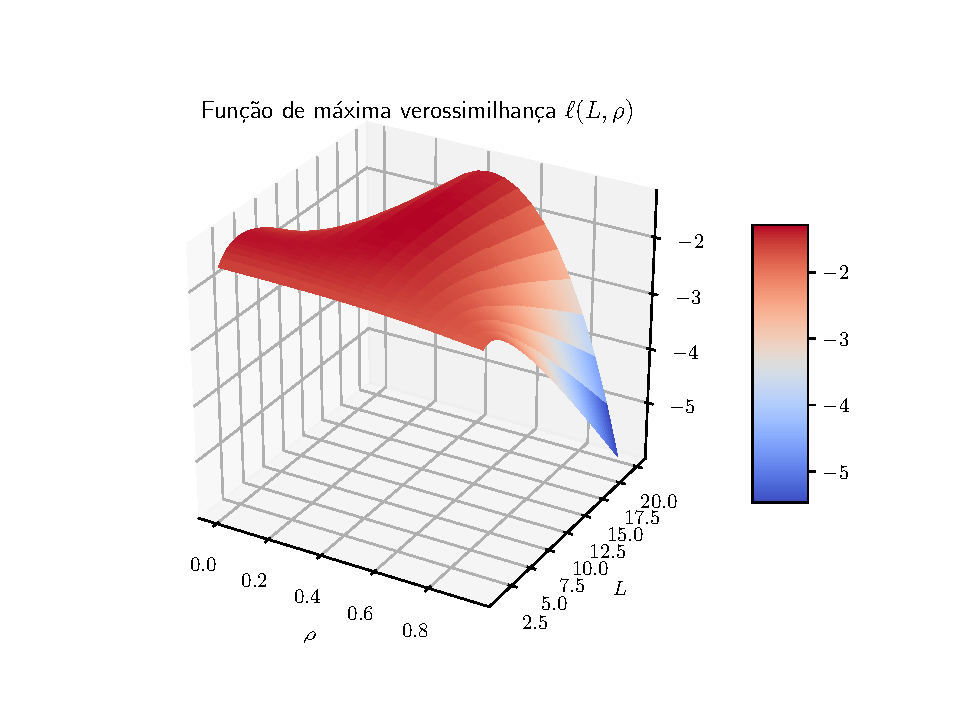
\includegraphics[width=0.50\linewidth]{fig_pdf_mag_prod_r_35_251_to_400}
     }
     \caption{Funções de máxima verossimilhança produto de magnitude com pixel fixo 250.}
     \label{fig:prod_mag_l_250_r_35} 
   \end{figure*}
   \begin{figure*}[hbt]
	\centering
     \subfloat[Pixel variando de 1 até 350 na linha 35.  \label{fig:prod_mag_l_rho_1_350}]{%
       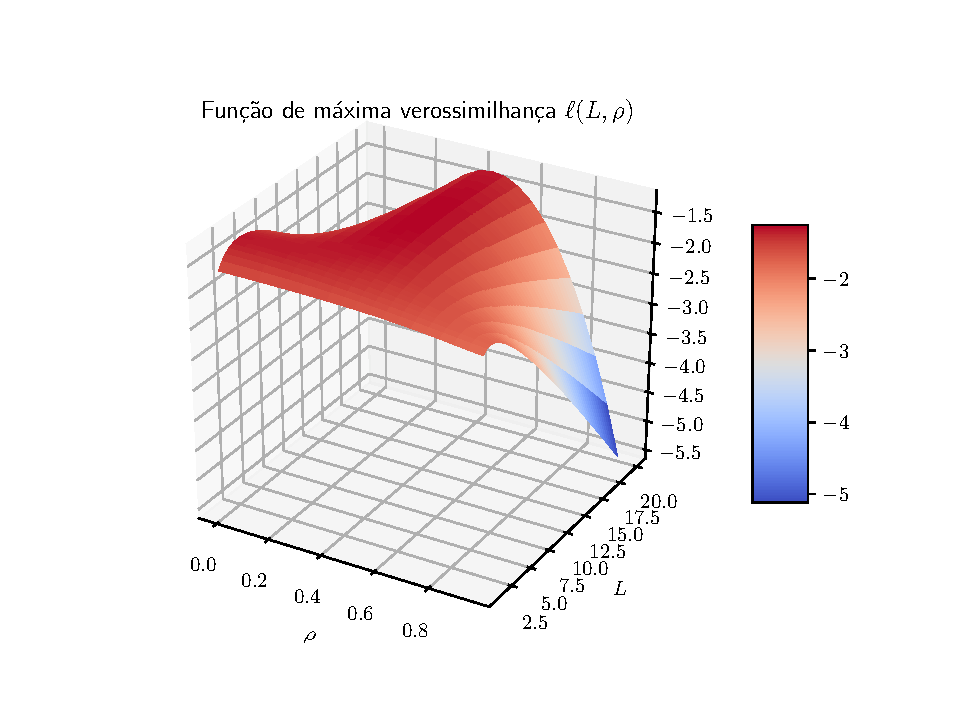
\includegraphics[width=0.50\linewidth]{fig_pdf_mag_prod_r_35_1_to_350}
     }
     \subfloat[Pixel variando de 351 até 400 na linha 35. \label{fig:prod_mag_l_rho_351_400}]{%
       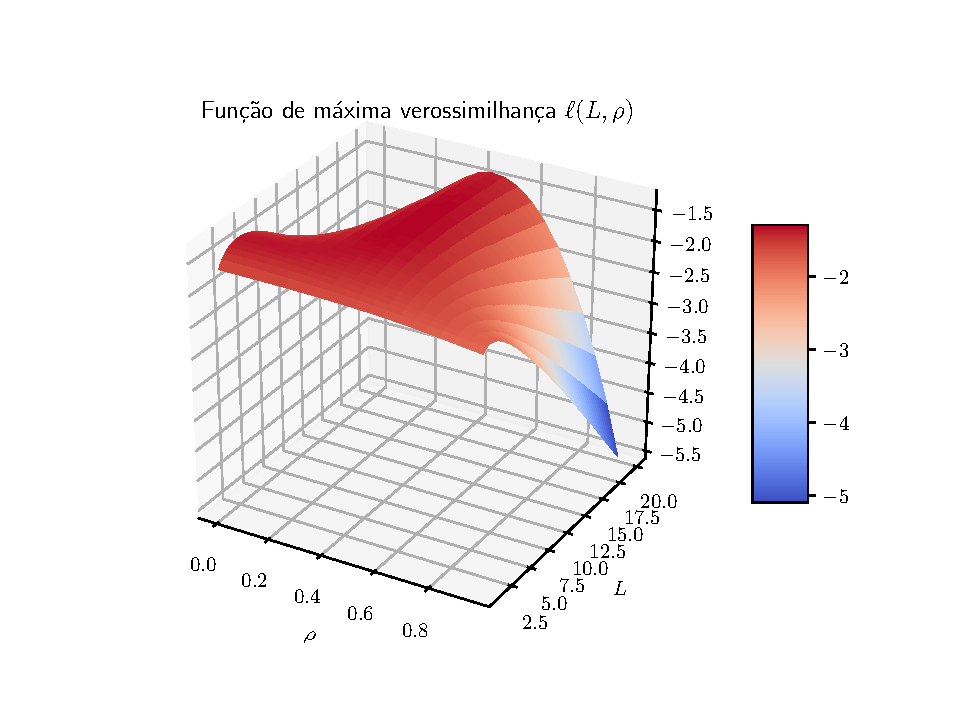
\includegraphics[width=0.50\linewidth]{fig_pdf_mag_prod_r_35_351_to_400}
     }
     \caption{Funções de máxima verossimilhança produto de magnitude com pixel fixo 350.}
     \label{fig:prod_mag_l_350_r_35} 
   \end{figure*}

As figuras \eqref{fig:prod_mag_l_25_r_50_hh}, \eqref{fig:prod_mag_l_25_r_50_hv} e \eqref{fig:prod_mag_l_25_r_50_vv} mostram a função de log-verossimilhança da pdf magnitude de produtos \eqref{eq:eq_log_vero_mag_prod_red} aplicada na ROI da imagem de flevoland. No processo fixamos arbitrariamente a radial 50 da amostra e fixamos o número de pixel 50. Desta maneira construímos duas funções $\ell{j}$ em cada lado da radial. Os gráficos das funções foram gerados para os canais de intensidades.



Na figura \eqref{fig:prod_mag_l_rho_1_25_hh} podemos identificar o problema da função ser plana dificultando muito o processo de encontrar o ponto de máximo gerando oscilação na função $\ell(j)$. Na \eqref{fig:prod_mag_l_rho_26_120_hh} ocorre o problema das funções de bessel serem infinitas quando seu argumento assume valores grande, também dificultando o cálculo do valor máximo.  

\begin{figure*}[hbt]
	\centering
     \subfloat[Pixel variando de 1 até 25 na radial 50 no canal (hh).  \label{fig:prod_mag_l_rho_1_25_hh}]{%
       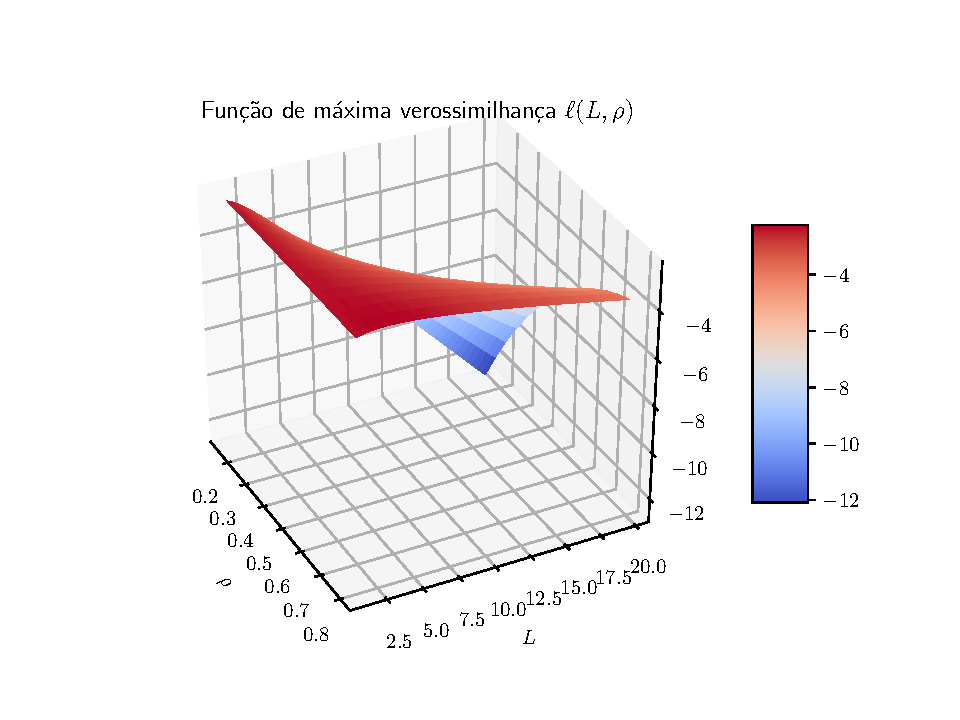
\includegraphics[width=0.50\linewidth]{fig_pdf_mag_prod_r_50_1_to_25_flev}
     }
     \subfloat[Pixel variando de 26 até 120 na radial 50 no canal (hh). \label{fig:prod_mag_l_rho_26_120_hh}]{%
       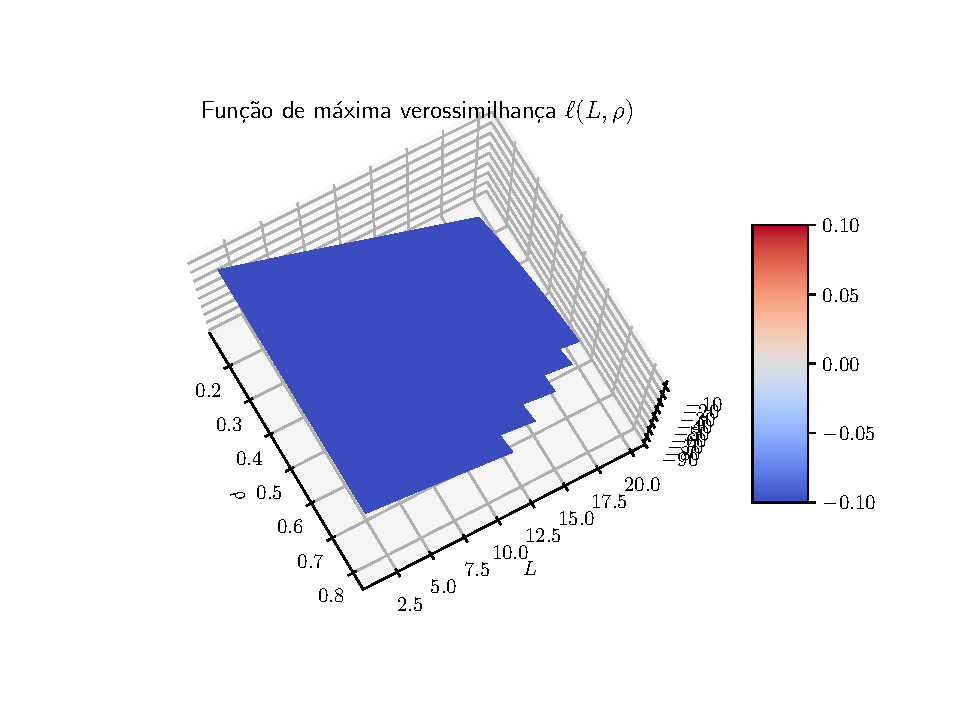
\includegraphics[width=0.50\linewidth]{fig_pdf_mag_prod_r_50_26_to_120_flev}
     }
     \caption{Funções de máxima verossimilhança produto de magnitude com pixel fixo 25 no canal (hh).}
     \label{fig:prod_mag_l_25_r_50_hh} 
   \end{figure*}
   

Nas figuras de \eqref{fig:prod_mag_l_25_r_50_hv} destacamos o problema da função ser plana. Assim como em no gráfico da função \eqref{fig:prod_mag_l_rho_1_25_hh} 


\begin{figure*}[hbt]
	\centering
     \subfloat[Pixel variando de 1 até 25 na radial 50 no canal (hv).  \label{fig:prod_mag_l_rho_1_25_hv}]{%
       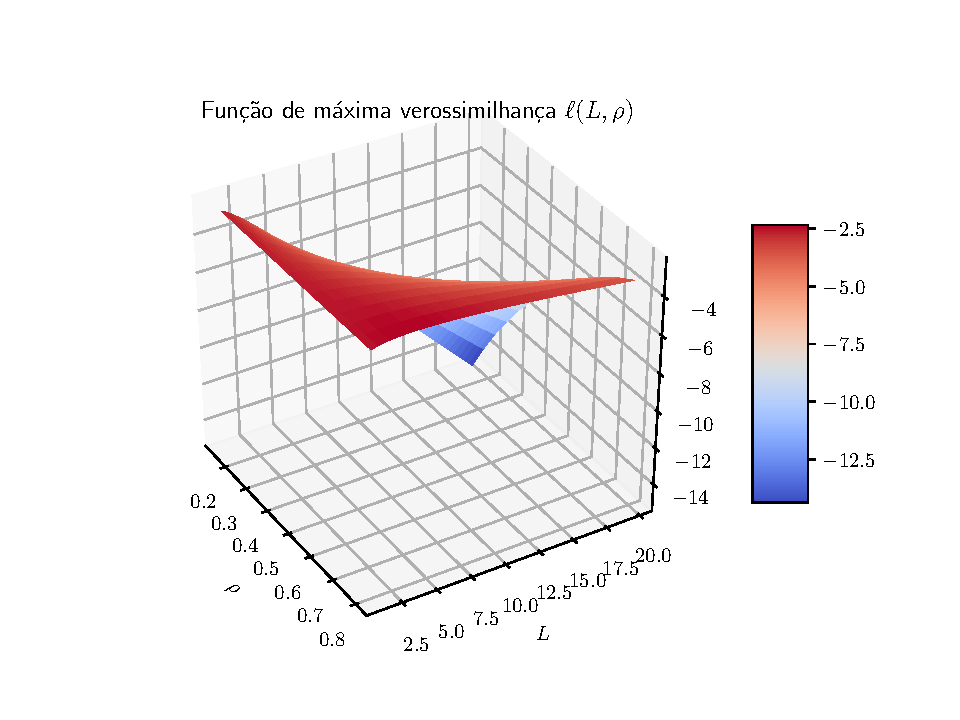
\includegraphics[width=0.50\linewidth]{fig_pdf_mag_prod_r_50_1_to_25_flev_hv}
     }
     \subfloat[Pixel variando de 26 até 120 na radial 50 no canal (hv). \label{fig:prod_mag_l_rho_26_120_hv}]{%
       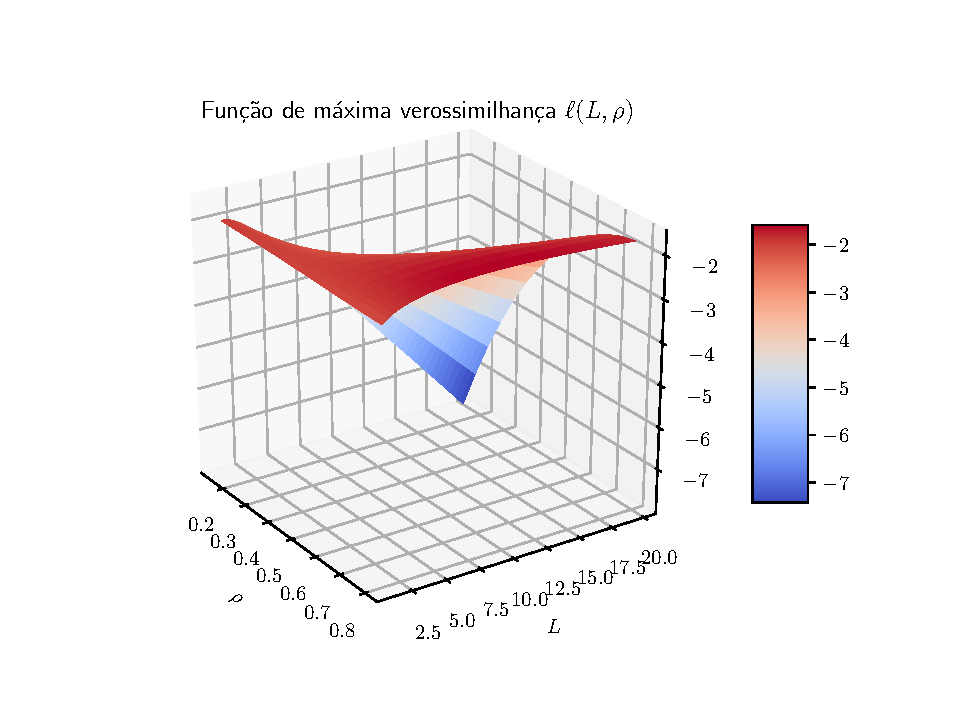
\includegraphics[width=0.50\linewidth]{fig_pdf_mag_prod_r_50_26_to_120_flev_hv}
     }
     \caption{Funções de máxima verossimilhança produto de magnitude com pixel fixo 25 no canal (hv).}
     \label{fig:prod_mag_l_25_r_50_hv} 
   \end{figure*}

Nas figuras de \eqref{fig:prod_mag_l_25_r_50_vv} destacamos o problema da função ser plana. Assim como em no gráfico da função \eqref{fig:prod_mag_l_rho_1_25_hh} 

\begin{figure*}[hbt]
	\centering
     \subfloat[Pixel variando de 1 até 25 na radial 50 no canal (vv).  \label{fig:prod_mag_l_rho_1_25_vv}]{%
       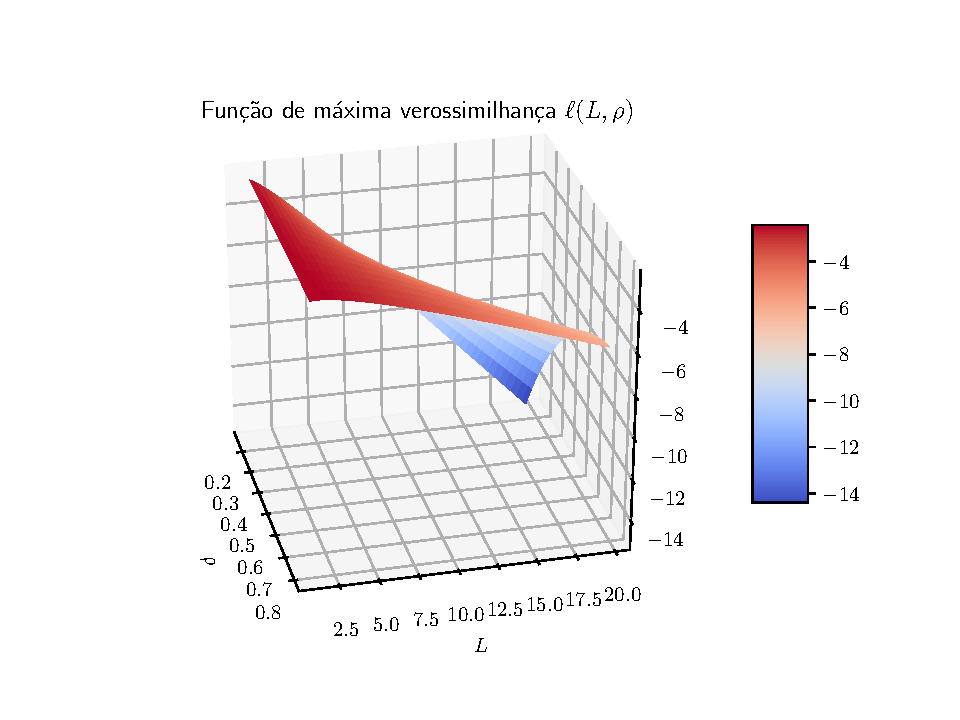
\includegraphics[width=0.50\linewidth]{fig_pdf_mag_prod_r_50_1_to_25_flev_vv}
     }
     \subfloat[Pixel variando de 26 até 120 na radial 50 no canal (vv). \label{fig:prod_mag_l_rho_26_120_vv}]{%
       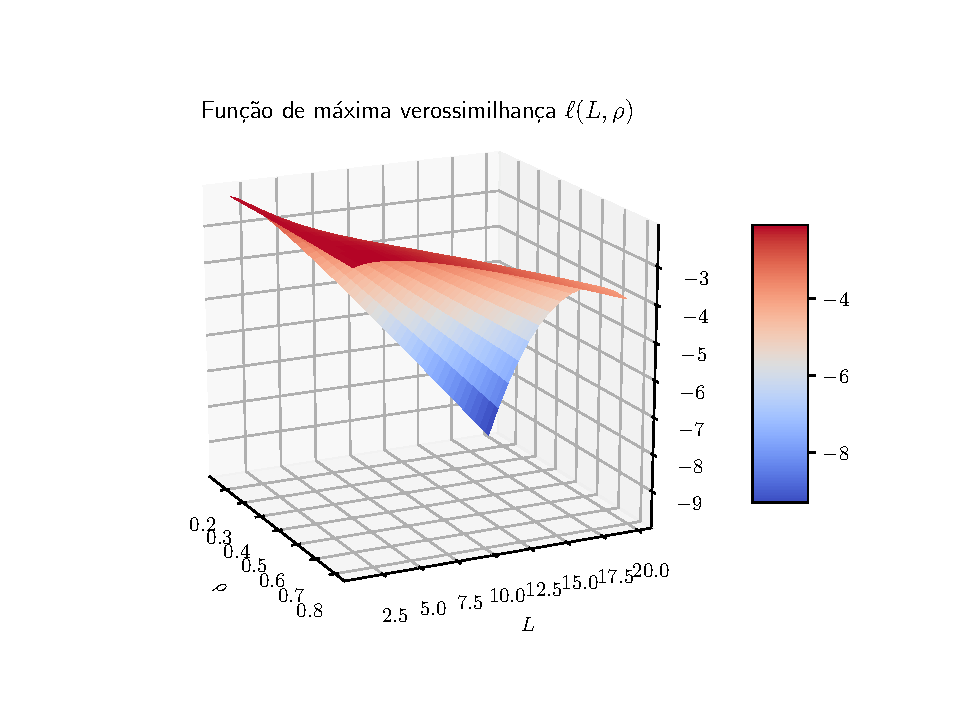
\includegraphics[width=0.50\linewidth]{fig_pdf_mag_prod_r_50_26_to_120_flev_vv}
     }
     \caption{Funções de máxima verossimilhança produto de magnitude com pixel fixo 25 no canal (vv).}
     \label{fig:prod_mag_l_25_r_50_vv} 
   \end{figure*}


Vamos obter $(\widehat \rho, \widehat L)$, o estimador de máxima verossimilhança (MLE) de $(\rho, L)$ baseado $\bm \xi$, por maximizar~\eqref{eq:eq_log_vero_mag_prod_red} com o método BFGS implementado no pacote \texttt{maxLik}~\citep{ht}. Preferimos otimizar resolvendo $\nabla\ell=\bm 0$ com objetivo de melhorar a estabilidade numérica do método.

A função otimizada é a log-verossimilhança reduzida para as amostras internas e externas da faixa de dados denotadas respectivamente como $\bm \xi_\text{I}$ e $\bm \xi_\text{E}$. Cada faixa de dados $\bm \xi = (\xi_1,\xi_2,\dots,\xi_n)$ é particionada em duas amostras disjuntas na posição $j$,  
$$
\bm \xi = (\underbrace{\xi_1,\xi_2,\dots,\xi_j}_{\bm \xi_\text{I}}, 
\underbrace{\xi_{j+1}, \xi_{j+2},\dots,\xi_n}_{\bm \xi_\text{E}}).
$$

Vamos estimar $(\rho_\text{I},L_\text{I})$ e $(\rho_\text{E},L_\text{E})$ com $\bm \xi_\text{I}$ e $\bm \xi_\text{E}$, maximizando~\eqref{eq:eq_log_vero_mag_prod_red}, e obtendo $(\widehat{\rho}_\text{I}, \widehat{L}_\text{I})$ e $(\widehat{\rho}_\text{E}, \widehat{L}_\text{E})$.

A log-verossimilhança no ponto $j$ é
\begin{equation}\label{eq:TotalLogLikelihood_prod_mag}
\begin{split}
\ell(j;\widehat{\rho}_\text{I}, \widehat{L}_\text{I}, \widehat{\rho}_\text{E}, \widehat{L}_\text{E})&
=j\left[(\widehat{L}_\text{I}+1)\ln \widehat{L}_\text{I}-\ln\Gamma(\widehat{L}_\text{I})-\ln(1-|\widehat{\rho}_\text{I}|^2)\right]
+\widehat{L}_\text{I}\sum_{k=1}^{j} \ln\xi_k\\
&+\sum_{k=1}^{j}\ln I_0\left(\frac{2|\widehat{\rho}_\text{I}|\widehat{L}_\text{I}\xi_k}{1-|\widehat{\rho}_\text{I}|^2}\right)
+ \sum_{k=1}^{j}\ln K_{\widehat{L}_\text{I}-1}\left(\frac{2\widehat{L}_\text{I}\xi_k}{1-|\widehat{\rho}_\text{I}|^2}\right)\\
&+(n-j)\left[(\widehat{L}_\text{E}+1)\ln \widehat{L}_\text{E}-\ln\Gamma(\widehat{L}_\text{E})-\ln(1-|\widehat{\rho}_\text{E}|^2)\right]
+\widehat{L}_\text{E}\sum_{k=j+1}^{n} \ln\xi_k\\
&+\sum_{k=j+1}^{n}\ln I_0\left(\frac{2|\widehat{\rho}_\text{E}|\widehat{L}_\text{E}\xi_k}{1-|\widehat{\rho}_\text{E}|^2}\right)
+ \sum_{k=j+1}^{n}\ln K_{\widehat{L}_\text{E}-1}\left(\frac{2\widehat{L}_\text{E}\xi_k}{1-|\widehat{\rho}_\text{E}|^2}\right).\\
\end{split}
\end{equation}

Vamos aplicar o método GenSA para encontrar
$$
\widehat{\jmath}= \arg\max\limits_{j\in [\min_s,N-\min_s]}\ell(j;\widehat{\rho}_I, \widehat{L}_I,\widehat{\rho}_E, \widehat{L}_E),
$$ 
onde $\min_s$ é o tamanho mínimo da amostra definido por $14$.

Podemos concluir que o uso da função densidade magnitude do produtos não é adequado para gerar a função log-verossimilhança. Essas funções resultantes tem características de serem planas dificultando o cálculo do valor máximo. O cálculo inadequado dos coeficientes $L$  e $\rho$ geram uma função \eqref{eq:TotalLogLikelihood_prod_mag} com muita oscilação degenerando o ponto onde o argumento é máximo.


\subsection{Método da verossimilhança aplicado na PDF univariada razão de intensidades múltiplas visadas}
A razão de intensidades ou amplitudes entre $\mathbf{S}_i$ e $\mathbf{S}_j$ são importantes no estudo de radares polarimétricos. Seja a razão de intensidade normalizada,
\begin{equation}\label{eq:razao_intensidades}
 \mu=\frac{\sum_{k=1}^{n}\frac{|\mathbf{S}_i(k)|^2}{\Sigma_{11}}}{\sum_{k=1}^{n}\frac{|\mathbf{S}_j(k)|^2}{\Sigma_{22}}}=\frac{\sum_{k=1}^{n}|\mathbf{S}_i(k)|^2}{\tau\sum_{k=1}^{n}|\mathbf{S}_j(k)|^2},\\
\end{equation}
onde $\tau=\frac{\Sigma_{11}}{\Sigma_{22}}$.
  
Considerando a função densidade de probabilidade univariada razão de intensidades múltiplas visadas,
\begin{equation}\label{eq:pdf_razao_intensidades}
	f(\mu;\rho,L)=\frac{\Gamma(2L)(1-|\rho|^2)^{L}(1+\mu)\mu^{L-1}}{\Gamma(L)\Gamma(L)\left[(1+\mu)^2-4|\rho|^2\mu \right]^{\frac{2L+1}{2}}}\\
\end{equation}
onde, $\rho>0$ e $L>0$. 
Podemos definir 
\begin{equation}\label{eq:razao_intensidades_w}
 w=\frac{\sum_{k=1}^{n}\frac{|\mathbf{S}_i(k)|^2}{\Sigma_{11}}}{\sum_{k=1}^{n}\frac{|\mathbf{S}_j(k)|^2}{\Sigma_{22}}}=\frac{\sum_{k=1}^{n}|\mathbf{S}_i(k)|^2}{\tau\sum_{k=1}^{n}|\mathbf{S}_j(k)|^2}=\tau \mu,\\ 
\end{equation}
realizando a mudança de variável na PDF, \eqref{eq:pdf_razao_intensidades} teremos, 
\begin{equation}\label{eq:pdf_razao_intensidades_tau_w}
	f(w;\rho,L,\tau)=\frac{\tau^L\Gamma(2L)(1-|\rho|^2)^{L}(\tau+w)w^{L-1}}{\Gamma(L)\Gamma(L)\left[(\tau+w)^2-4\tau|\rho|^2w \right]^{\frac{2L+1}{2}}}\\
\end{equation}

Aplicando o logaritmo natural na equação~\eqref{eq:pdf_razao_intensidades_tau_w} e realizando algumas manipulações algébricas teremos:

\begin{equation}\nonumber
\begin{split}
	\ln f(w;\rho,L,\tau)&=\ln\left(\frac{\tau^L\Gamma(2L)(1-|\rho|^2)^{L}(\tau+w)w^{L-1}}{\Gamma(L)\Gamma(L)\left[(\tau+w)^2-4\tau|\rho|^2w \right]^{\frac{2L+1}{2}}}\right),\\
	                &=\ln\left(\tau^L\Gamma(2L)(1-|\rho|^2)^{L}(\tau+w)w^{L-1}\right)\\
	                &-\ln\left(\Gamma(L)\Gamma(L)\left[(\tau+w)^2-4\tau|\rho|^2w \right]^{\frac{2L+1}{2}}\right),\\
	                &=\ln\tau^L + \ln\Gamma(2L) +\ln(1-|\rho|^2)^{L}+\ln(\tau+w)+\ln w^{L-1}\\
	                &-\left(\ln\Gamma(L)+\ln\Gamma(L)+\ln\left[(\tau+w)^2-4\tau|\rho|^2w \right]^{\frac{2L+1}{2}}\right),\\
	                &=L\ln\tau + \ln\Gamma(2L) +L\ln(1-|\rho|^2)+\ln(\tau+w)+(L-1)\ln w\\
	                &-2\ln\Gamma(L)-\frac{2L+1}{2}\ln\left[(\tau+w)^2-4\tau|\rho|^2w \right].\\
\end{split}
\end{equation}

Definimos a equação log-verossimilhança para a PDF univariada razão de intensidades múltiplas visadas,
\begin{equation}\label{eq_log_vero_razao_intensidade_tau_w}
\begin{split}	
	\ln f(w;\rho,L,\tau)&=L\ln\tau + \ln\Gamma(2L) +L\ln(1-|\rho|^2)+\ln(\tau+w)+(L-1)\ln w\\
	                      &-2\ln\Gamma(L)-\frac{2L+1}{2}\ln\left[(\tau+w)^2-4\tau|\rho|^2w \right].\\
\end{split}
\end{equation}

A função log-verossimilhança pode ser deduzida da seguinte maneira, dado a amostra $\bm w = (w_1,\dots,w_n)$, 
\begin{equation}\nonumber
\begin{split}
  \ell(\bm w;\rho, L)=\ln\prod_{k=1}^{n}f(w_k;\rho,L)\\
  \ell(\bm w;\rho, L)=\sum_{k=1}^{n}\ln f(w_k;\rho,L),
 \end{split}
 \end{equation}
usando a função~\eqref{eq_log_vero_razao_intensidade_tau_w} teremos,
\begin{equation}\nonumber
\begin{split}
    \ell(\bm w;\rho, L, \tau)&=\sum_{k=1}^{n}\ln f(\mu_k;\rho, L)\\
                         &=\sum_{k=1}^{n}\left[L\ln\tau + \ln\Gamma(2L) +L\ln(1-|\rho|^2)+\ln(\tau+w)+(L-1)\ln w\right.\\
	                     &-\left.2\ln\Gamma(L)-\frac{2L+1}{2}\ln\left[(\tau+w)^2-4\tau|\rho|^2w \right]\right].\\
 \end{split}
 \end{equation}
 
 \begin{equation}\nonumber
\begin{split} 
    \ell(\bm w;\rho, L, \tau)&=L\ln\tau\sum_{k=1}^{n}1+\ln\Gamma(2L)\sum_{k=1}^{n} 1+L\ln(1-|\rho|^2)\sum_{k=1}^{n} 1+\sum_{k=1}^{n}\ln(\tau+w_k)+(L-1)\sum_{k=1}^{n}\ln w_k\\
                         &-2\ln\Gamma(L)\sum_{k=1}^{n} 1-\frac{2L+1}{2}\sum_{k=1}^{n}\ln\left[(\tau+w_k)^2-4\tau|\rho|^2w_k\right]\\
                         &=n\left(L\ln\tau+\ln\Gamma(2L)+L\ln(1-|\rho|^2)-2\ln\Gamma(L)\right)+\sum_{k=1}^{n}\ln(\tau+w_k)\\
                         &+L\sum_{k=1}^{n}\ln w_k-\sum_{k=1}^{n}\ln w_k-\frac{2L+1}{2}\sum_{k=1}^{n} \ln\left[(\tau+ w_k)^2-4\tau|\rho|^2w_k\right].\\
\end{split}
\end{equation}
 
Definimos a equação log-verossimilhança para a PDF univariada~(\ref{eq_log_vero_razao_intensidade_tau_w}).
\begin{equation}\nonumber
\begin{split}
    \ell(\bm w;\rho, L, \tau)&=n\left(L\ln\tau + \ln\Gamma(2L)+L\ln(1-|\rho|^2)-2\ln\Gamma(L)\right)+\sum_{k=1}^{n}\ln(\tau+w_k)\\
                         &+L\sum_{k=1}^{n}\ln w_k-\sum_{k=1}^{n}\ln w_k-\frac{2L+1}{2}\sum_{k=1}^{n} \ln\left[(\tau+w_k)^2-4\tau|\rho|^2w_k\right]\\
\end{split}
 \end{equation}
e a forma reduzida,
\begin{equation}\label{eq_log_vero_razao_intensidade_red_tau_w}
\begin{split}
    \ell(\bm w;\rho, L, \tau)&=n\left(L\ln\tau +\ln\Gamma(2L)+L\ln(1-|\rho|^2)-2\ln\Gamma(L)\right)\\
                         &+\sum_{k=1}^{n}\ln(\tau+w_k)+L\sum_{k=1}^{n}\ln w_k-\frac{2L+1}{2}\sum_{k=1}^{n} \ln\left[(\tau+w_k)^2-4\tau|\rho|^2w_k\right]\\
\end{split}
 \end{equation} 

Vamos obter $(\widehat \rho, \widehat L, \widehat \tau)$, o estimador de máxima verossimilhança (MLE) de $(\rho, L, \tau)$ baseado em $\bm w$ maximizando~\eqref{eq_log_vero_razao_intensidade_red_tau_w} com o método BFGS implementado no pacote \texttt{maxLik}~\citep{ht}. Vamos preferir otimização resolvendo $\nabla\ell=\bm 0$ com intuito de melhorar a estabilidade numérica.

A função é a log-verossimilhança reduzida para as amostras internas e externas da faixa de dados denotadas respectivamente como $\bm w_\text{I}$ e $\bm w_\text{E}$. Cada faixa de dados $\bm w = (w_1,w_2,\dots,w_n)$ é particionada em duas amostras disjuntas na posição $j$:  
$$
\bm w = (\underbrace{w_1,w_2,\dots,w_j}_{\bm w_\text{I}}, 
\underbrace{w_{j+1}, w_{j+2},\dots,w_n}_{\bm w_\text{E}}).
$$
%Vamos assumir dois diferentes modelos para cada partição:
%$\bm Z_\text{I} \sim \Gamma(\mu_\text{I},L_\text{I})$, e
%$\bm Z_\text{E} \sim \Gamma(\mu_\text{E},L_\text{E})$.
Vamos estimar $(\rho_\text{I},L_\text{I}, \tau_\text{I})$ e $(\rho_\text{E},L_\text{E}, \tau_\text{E})$ com $\bm w_\text{I}$ e $\bm w_\text{E}$, respectivamente, maximizando~\eqref{eq:eq_log_vero_mag_prod_red}, e obtendo $(\widehat{\rho}_\text{I}, \widehat{L}_\text{I}, \widehat{\tau}_\text{I})$ e $(\widehat{\rho}_\text{E}, \widehat{L}_\text{E}, \widehat{\tau}_\text{E})$.

A log-verossimilhança no ponto $j$ é, então
\begin{equation}\label{eq:TotalLogLikelihood}
\begin{split}
\ell(j;\widehat{\rho}_\text{I}, \widehat{L}_\text{I}, \widehat{\tau}_\text{I}, \widehat{\rho}_\text{E}, \widehat{L}_\text{E},\widehat{\tau}_\text{E})&=n\left(\widehat{L}_\text{I}\ln\widehat{\tau}_\text{I} +\ln\Gamma(2\widehat{L}_\text{I})+\widehat{L}_\text{I}\ln(1-|\widehat{\rho}_\text{I}|^2)-2\ln\Gamma(\widehat{L}_\text{I})\right)\\
                         &+\sum_{k=1}^{n}\ln(\widehat{\tau}_\text{I}+w_k)+\widehat{L}_\text{I}\sum_{k=1}^{n}\ln w_k-\frac{2\widehat{L}_\text{I}+1}{2}\sum_{k=1}^{n} \ln\left[(\widehat{\tau}_\text{I}+w_k)^2-4\widehat{\tau}_\text{I}|\widehat{\rho}_{I}|^2w_k\right]\\
                         &+n\left(\widehat{L}_\text{E}\ln\widehat{\tau}_\text{E}+\ln\Gamma(2\widehat{L}_\text{E})+\widehat{L}_\text{E}\ln(1-|\widehat{\rho}_\text{E}|^2)-2\ln\Gamma(\widehat{L}_\text{E})\right)\\
                         &+\sum_{k=1}^{n}\ln(\widehat{\tau}_\text{E}+w_k)+\widehat{L}_\text{E}\sum_{k=1}^{n}\ln w_k-\frac{2\widehat{L}_\text{E}+1}{2}\sum_{k=1}^{n} \ln\left[(\widehat{\tau}_\text{E}+w_k)^2-4\widehat{\tau}_\text{E}|\widehat{\rho}_\text{E}|^2w_k\right]
%\raisetag{2.2em}
\end{split}
\end{equation}

Vamos aplicar o método GenSA para encontrar
$$
\widehat{\jmath}= \arg\max\limits_{j\in [\min_s,N-\min_s]}\ell(j;\widehat{\rho}_I, \widehat{L}_I,\widehat{\tau}_I,\widehat{\rho}_E, \widehat{L}_E, \widehat{\tau}_E),
$$ 
onde $\min_s$ é o tamanho mínimo da amostra definido por $14$.

Desta maneira, vamos obter uma estimativa para a borda em cada canal de intensidade.
Note que esse método pode ser estendido e/ou modificado para lidar com qualquer tipo de dados.

\subsubsection{Aplicação na imagem simulada com duas amostras}


As figuras \eqref{fig:razao_tau_rho_1_50} até \eqref{fig:razao_tau_rho_51_400} mostram a função de log-verossimilhança da pdf razão de intensidades \eqref{eq:pdf_razao_intensidades_tau_w} aplicada na imagem de duas amostras simulada. No processo fixamos arbitrariamente a linha 80 da amostra e variamos o número de pixel entre 50, 150, 250 e 250. Desta maneira construímos duas funções $\ell{j}$, uma para cada lado da amostra. Nessas figuras fixamos o L = 4 e os canais (hh) e (vv).
 \begin{figure*}[hbt]
	\centering
     \subfloat[Pixel variando de 1 até 50 na linha 80.  \label{fig:razao_tau_rho_1_50}]{%
       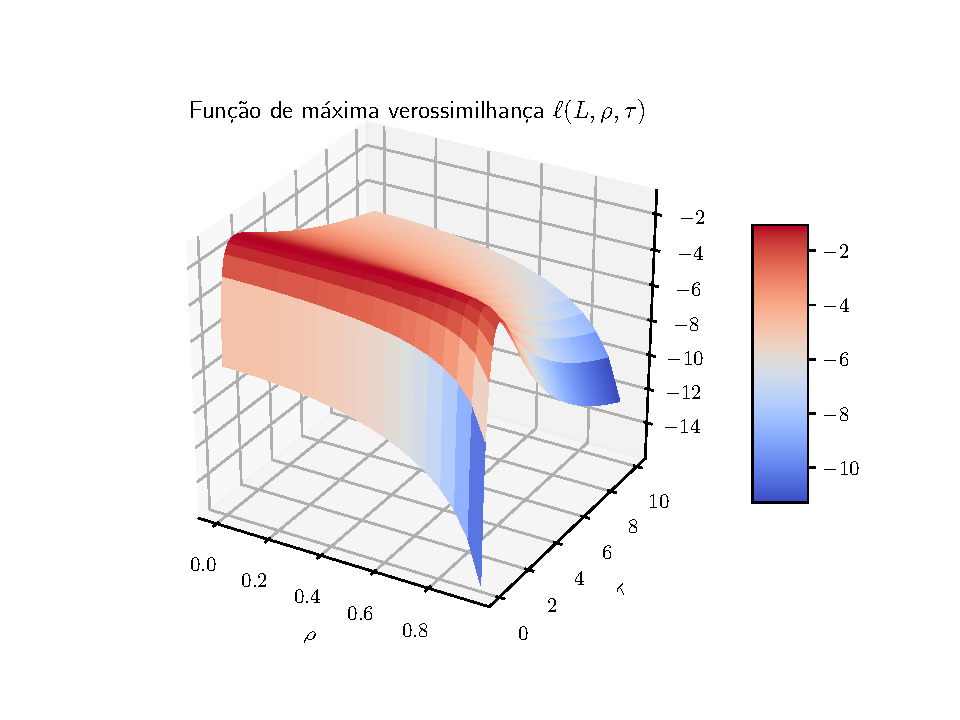
\includegraphics[width=0.50\linewidth]{fig_pdf_razao_r_80_1_to_50}
     }
     \subfloat[Pixel variando de 51 até 400 na linha 80. \label{fig:razao_tau_rho_51_400}]{%
       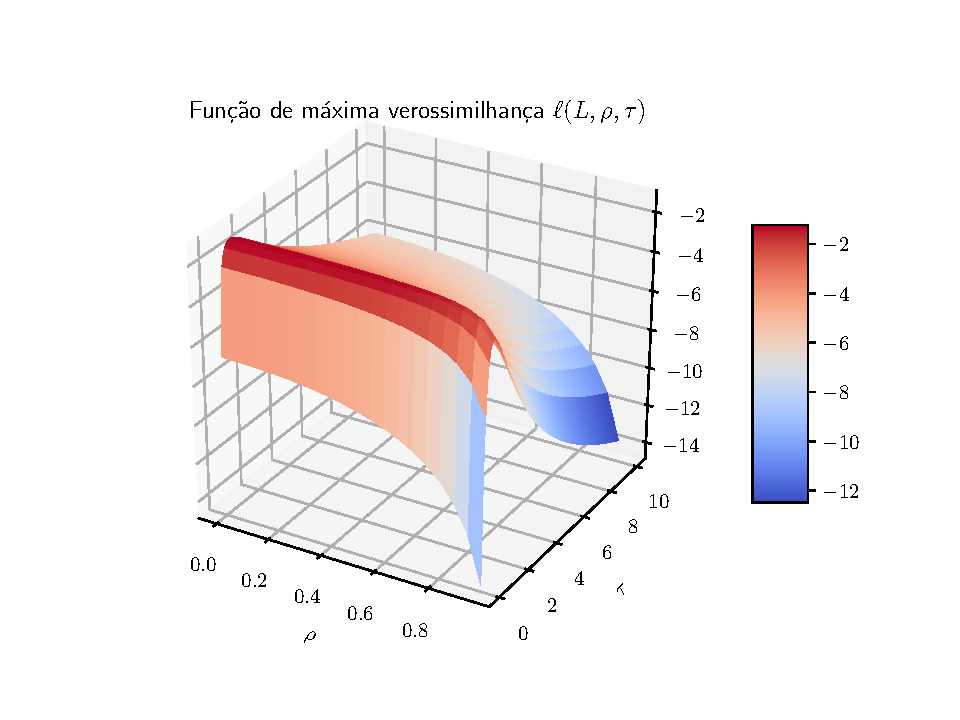
\includegraphics[width=0.50\linewidth]{fig_pdf_razao_r_80_50_to_400}
     }
     \caption{Funções de máxima verossimilhança razão de intensidades com pixel fixo 50.}
     \label{fig:razao_l_50_r_80} 
   \end{figure*}
\begin{figure*}[hbt]
	\centering
     \subfloat[Pixel variando de 1 até 150 na linha 80.  \label{fig:razao_tau_rho_1_150}]{%
       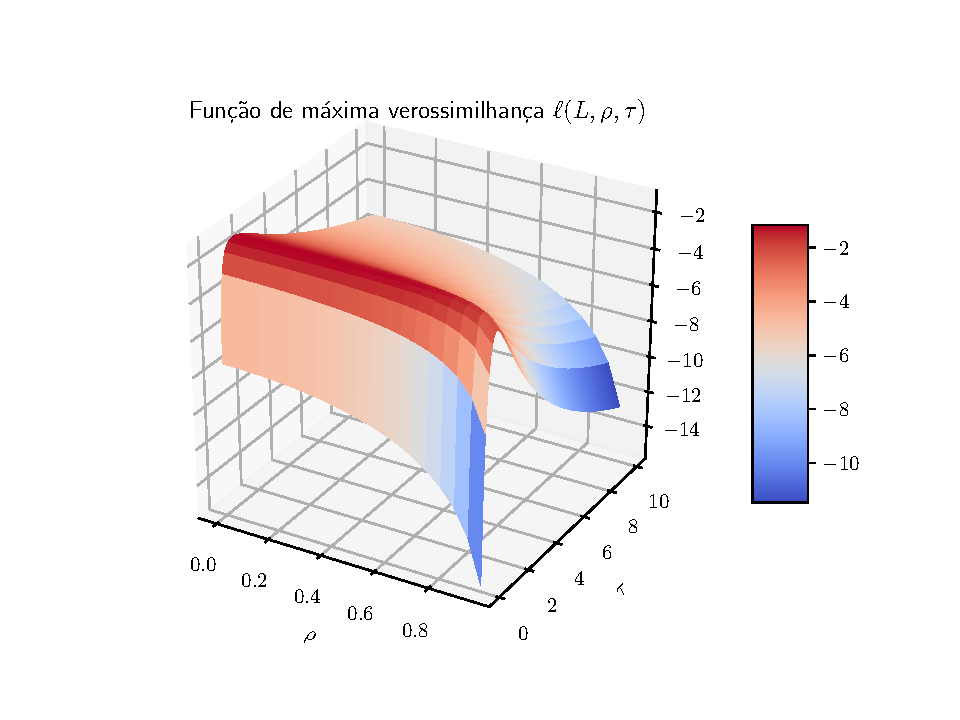
\includegraphics[width=0.50\linewidth]{fig_pdf_razao_r_80_1_to_150}
     }
     \subfloat[Pixel variando de 151 até 400 na linha 80. \label{fig:razao_tau_rho_151_400}]{%
       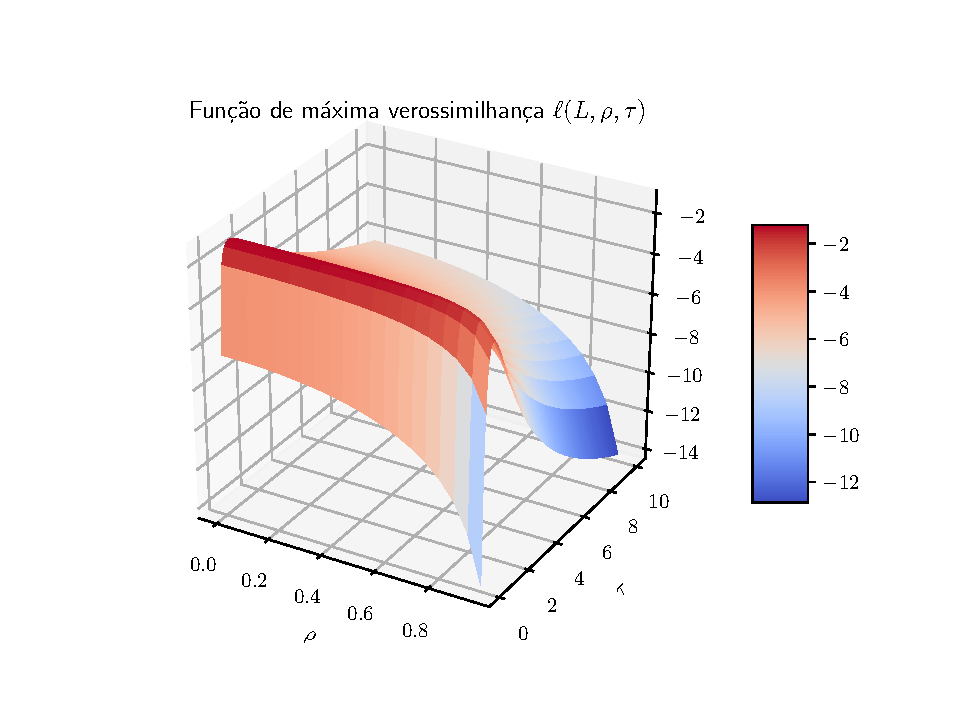
\includegraphics[width=0.50\linewidth]{fig_pdf_razao_r_80_150_to_400}
     }
     \caption{Funções de máxima verossimilhança razão de intensidades com pixel fixo 150.}
     \label{fig:razao_l_150_r_80} 
   \end{figure*}   
   
   \begin{figure*}[hbt]
	\centering
     \subfloat[Pixel variando de 1 até 250 na linha 80.  \label{fig:razao_tau_rho_1_250}]{%
       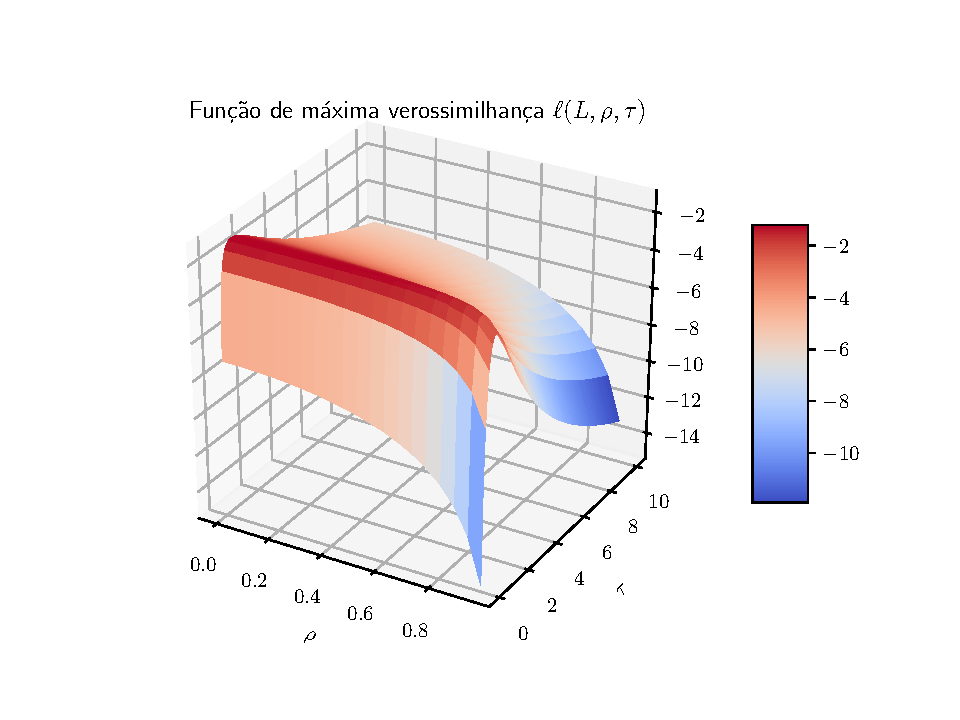
\includegraphics[width=0.50\linewidth]{fig_pdf_razao_r_80_1_to_250}
     }
     \subfloat[Pixel variando de 251 até 400 na linha 80. \label{fig:razao_tau_rho_251_400}]{%
       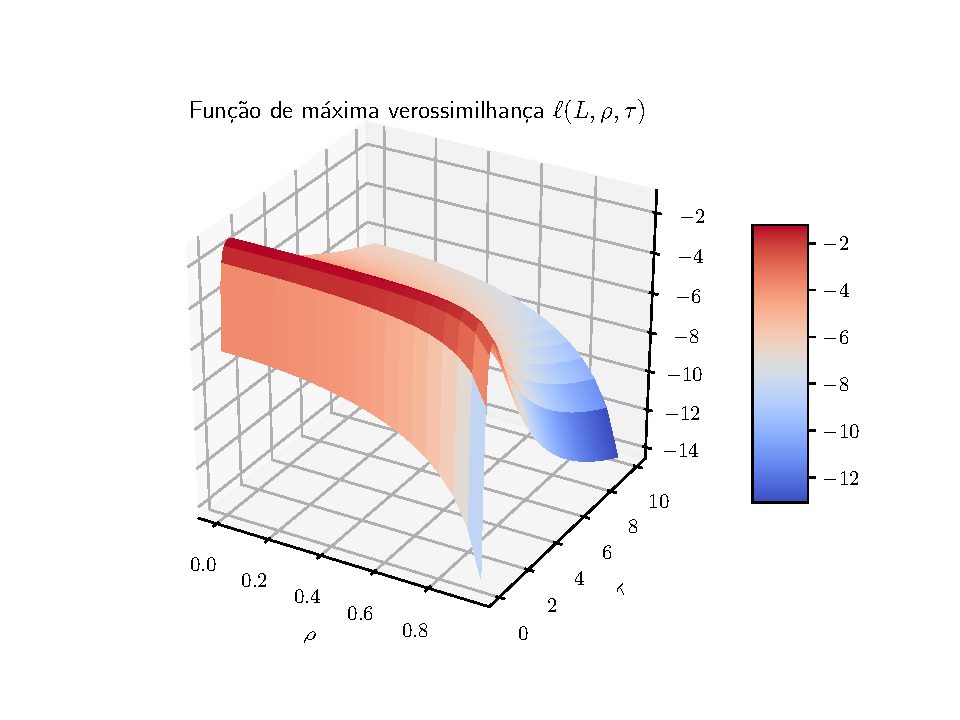
\includegraphics[width=0.50\linewidth]{fig_pdf_razao_r_80_250_to_400}
     }
     \caption{Funções de máxima verossimilhança razão de intensidades com pixel fixo 250.}
     \label{fig:razao_l_250_r_80} 
   \end{figure*}   
   
   \begin{figure*}[hbt]
	\centering
     \subfloat[Pixel variando de 1 até 350 na linha 80.  \label{fig:razao_tau_rho_1_350}]{%
       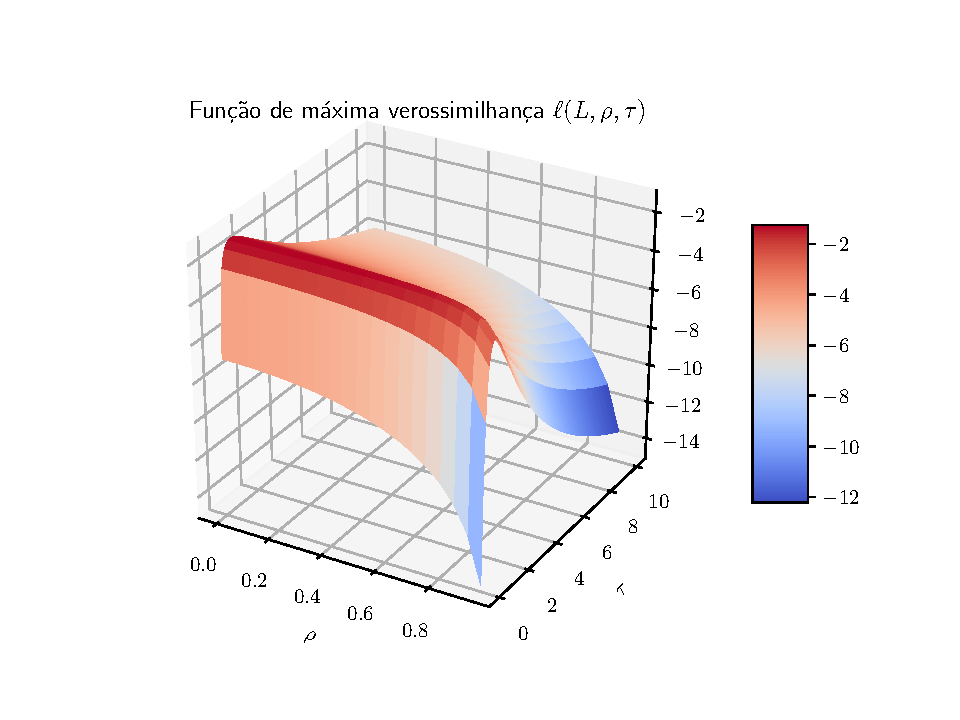
\includegraphics[width=0.50\linewidth]{fig_pdf_razao_r_80_1_to_350}
     }
     \subfloat[Pixel variando de 351 até 400 na linha 80. \label{fig:razao_tau_rho_351_400}]{%
       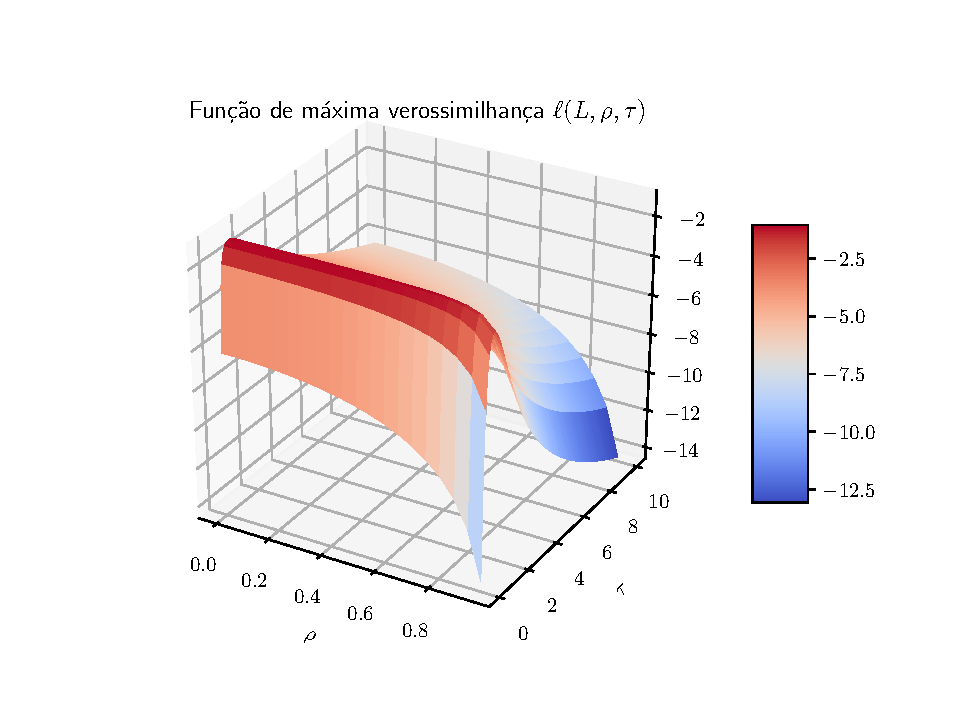
\includegraphics[width=0.50\linewidth]{fig_pdf_razao_r_80_350_to_400}
     }
     \caption{Funções de máxima verossimilhança razão de intensidades com pixel fixo 350.}
     \label{fig:razao_l_250_r_80} 
   \end{figure*}   
   

O método da máxima verossimilhança \eqref{eq:TotalLogLikelihood} foi aplicado na imagem simulada com duas amostras, e as evidências de bordas estão mostradas na figura. \textcolor{red}{Base de dados gamf}
 \begin{figure*}[hbt]
	\centering
     \subfloat[Evidências no canal $\text{hh}$ \label{evidencias_hh_hv_vv_gamf:a}]{%
       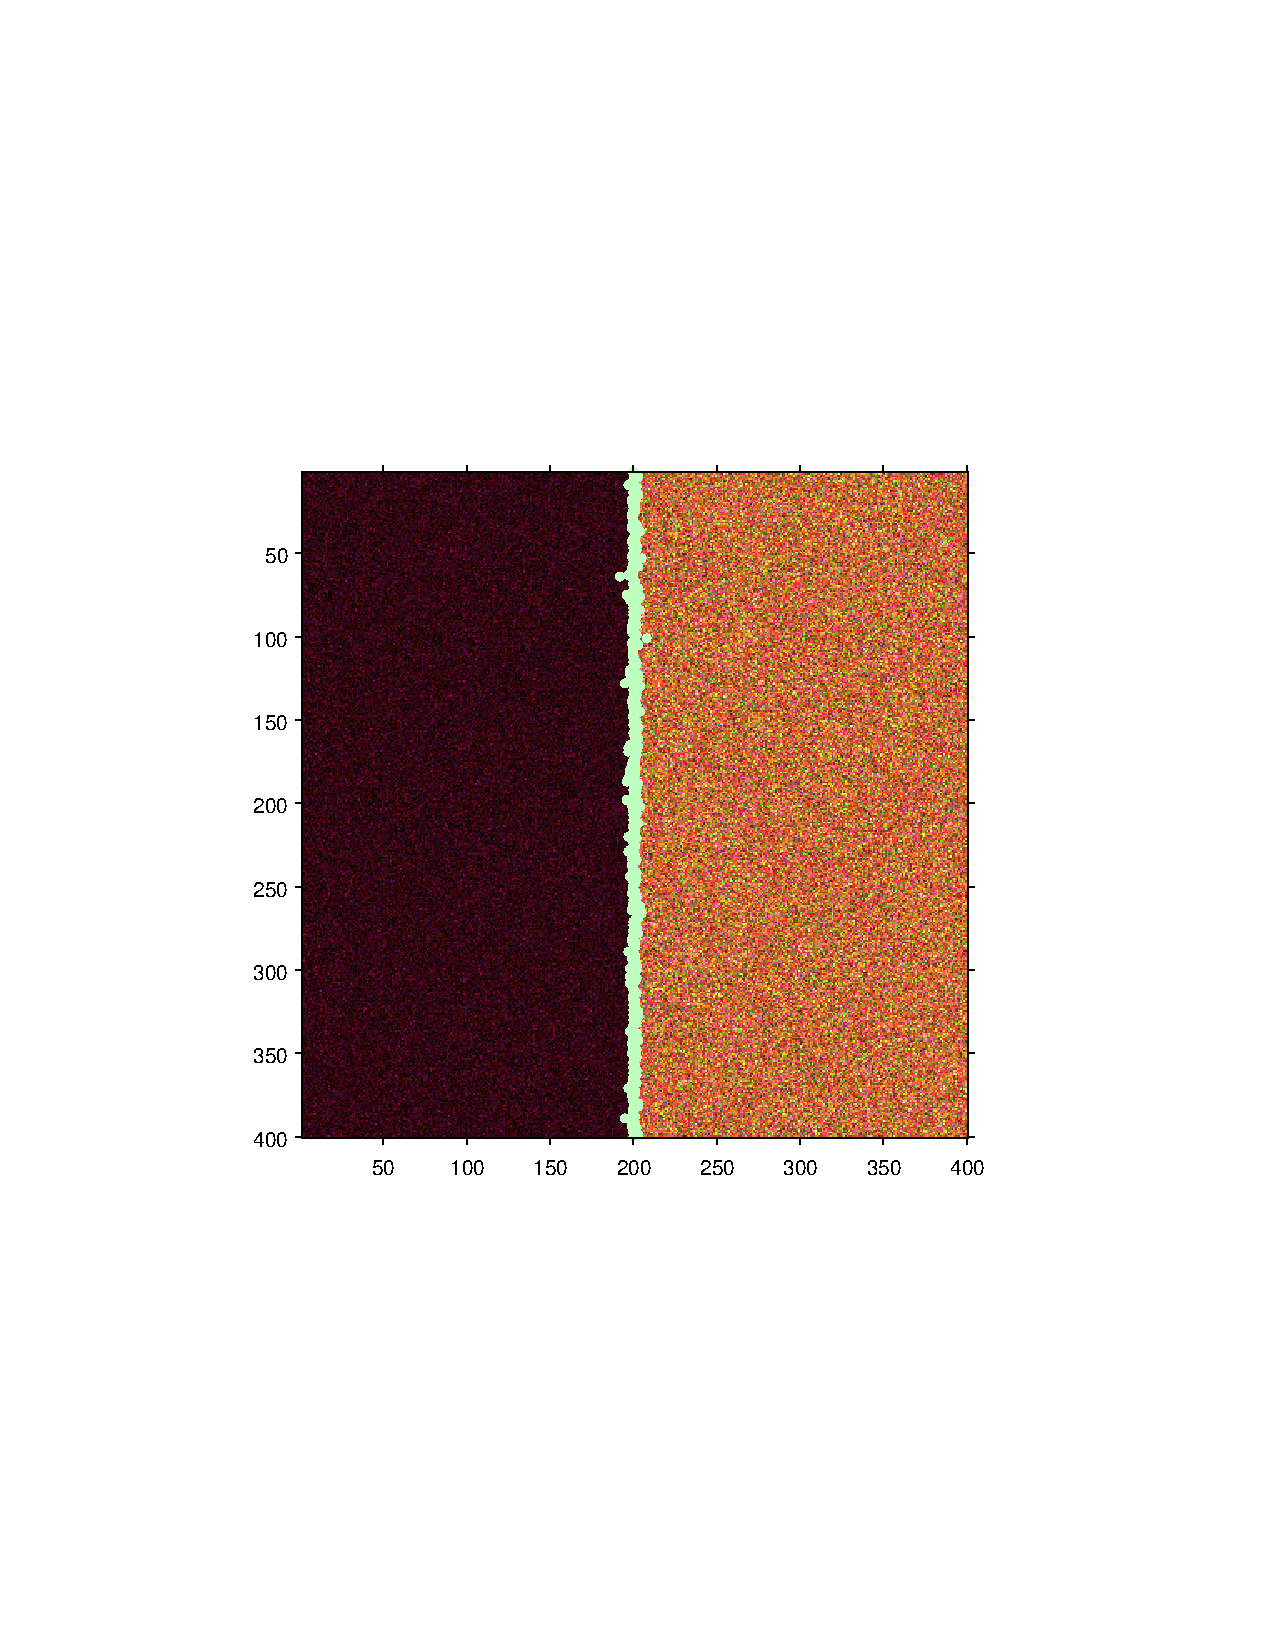
\includegraphics[width=0.5\linewidth]{im_sim_gamf_hh_hv_param_tau_rho_14_pixel}
     }
     \subfloat[xxxxxxxxxxxxxxxxxx $\text{hv}$ \label{evidencias_hh_hv_vv_gamf:b}]{%
       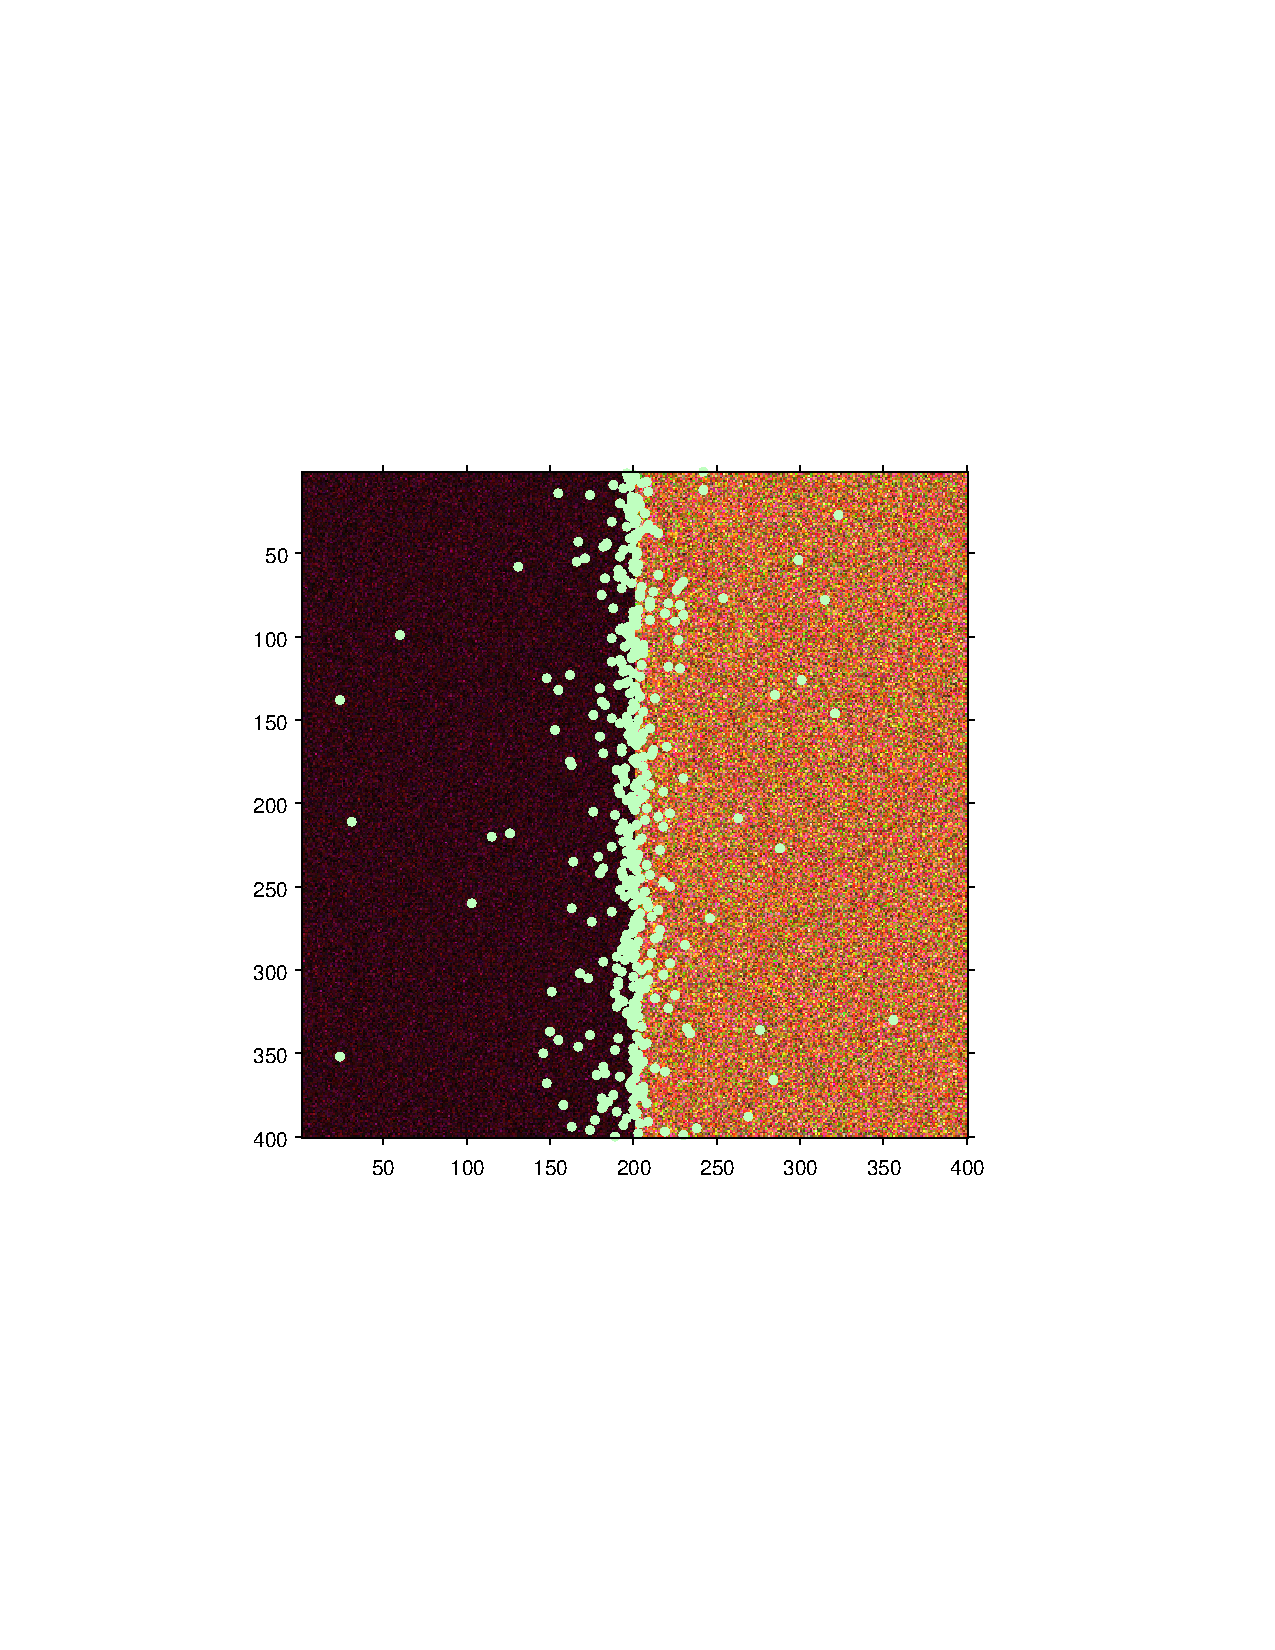
\includegraphics[width=0.5\linewidth]{im_sim_gamf_hh_vv_param_tau_rho_14_pixel}
     }      
   %  \subfloat[Evidências no canal $\text{vv}$ \label{evidencias_hh_hv_vv_gamf:c}]{%
    %   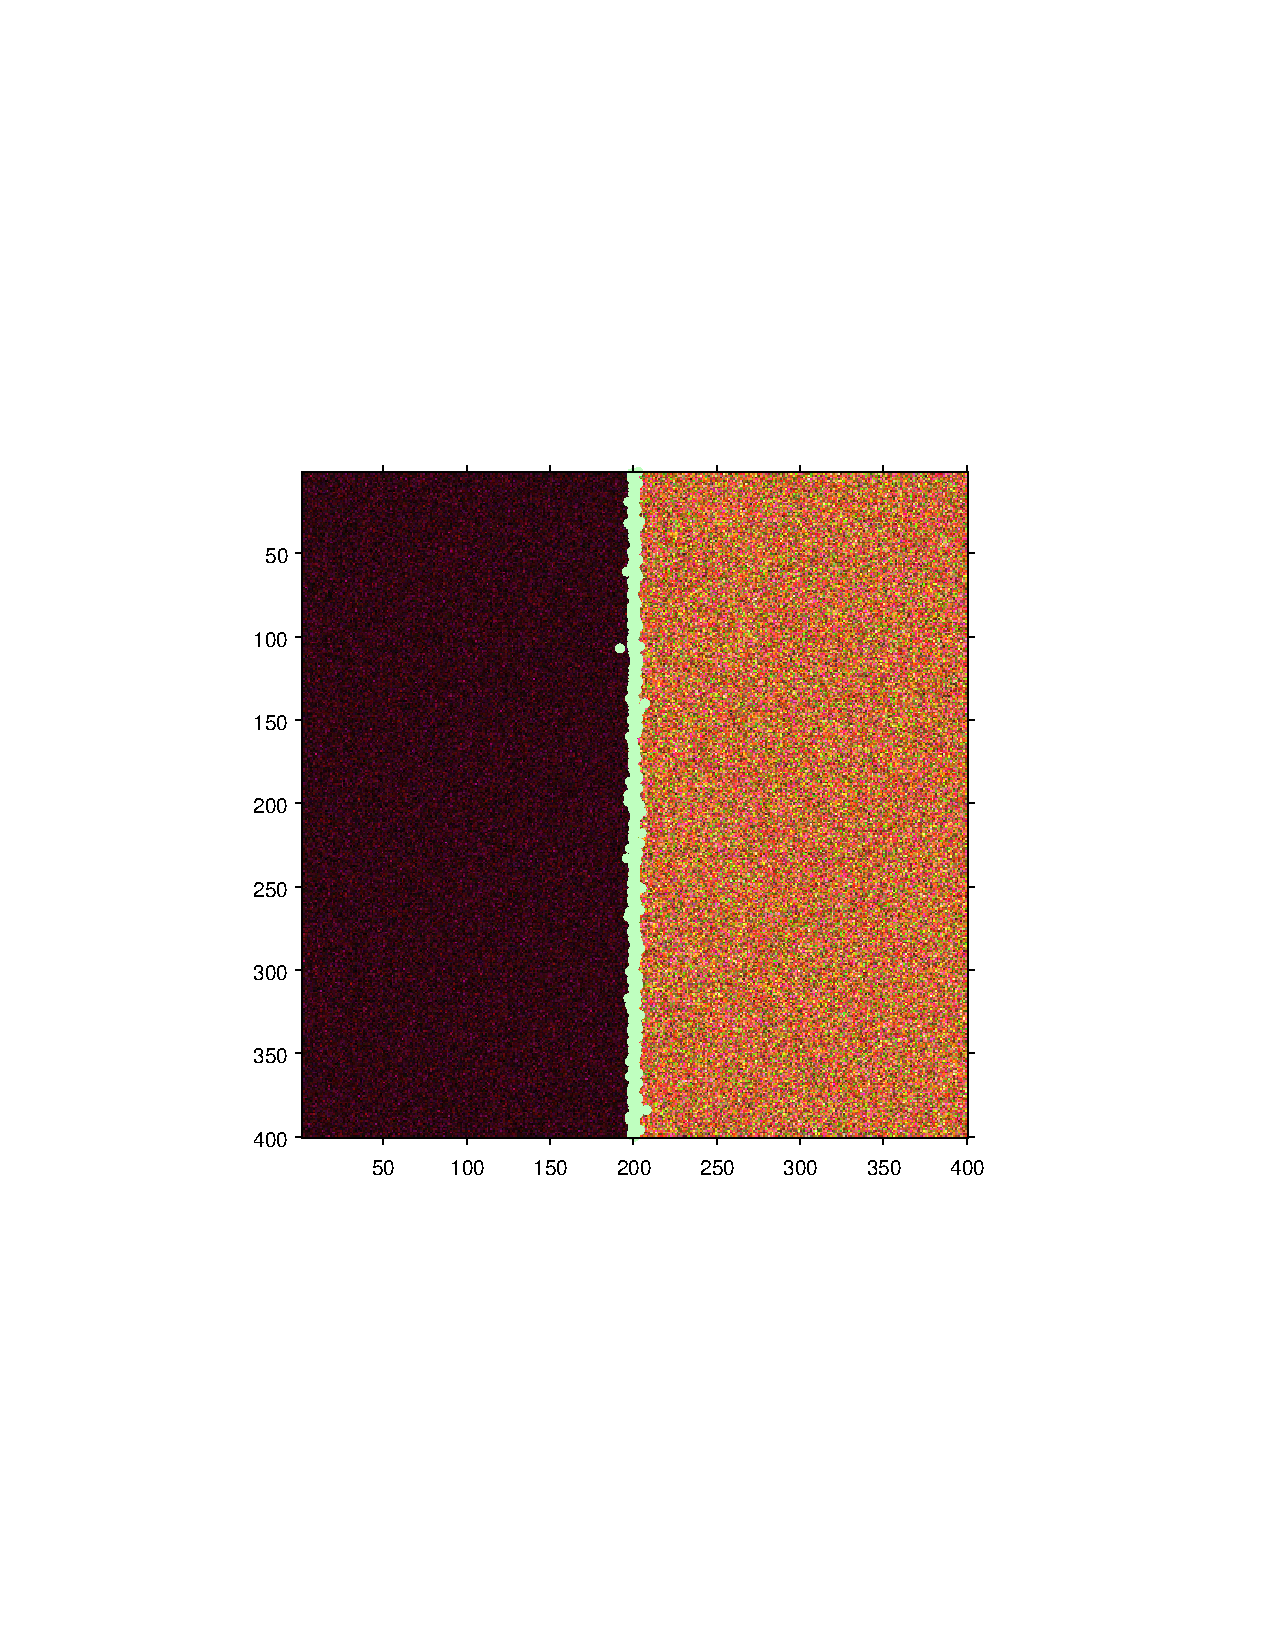
\includegraphics[width=0.5\linewidth]{im_sim_gamf_hh_evid_param_L_mu_14_pixel}
    % }
    \caption{Evidências de bordas para os três canais de intensidade}
     \label{evidencias_hh_hv_vv_gamf} 
   \end{figure*}
   
   \begin{figure*}[hbt]
	\centering
     \subfloat[Evidências no canal $\text{vv}$ \label{evidencias_hh_hv_vv_gamf:c}]{%
       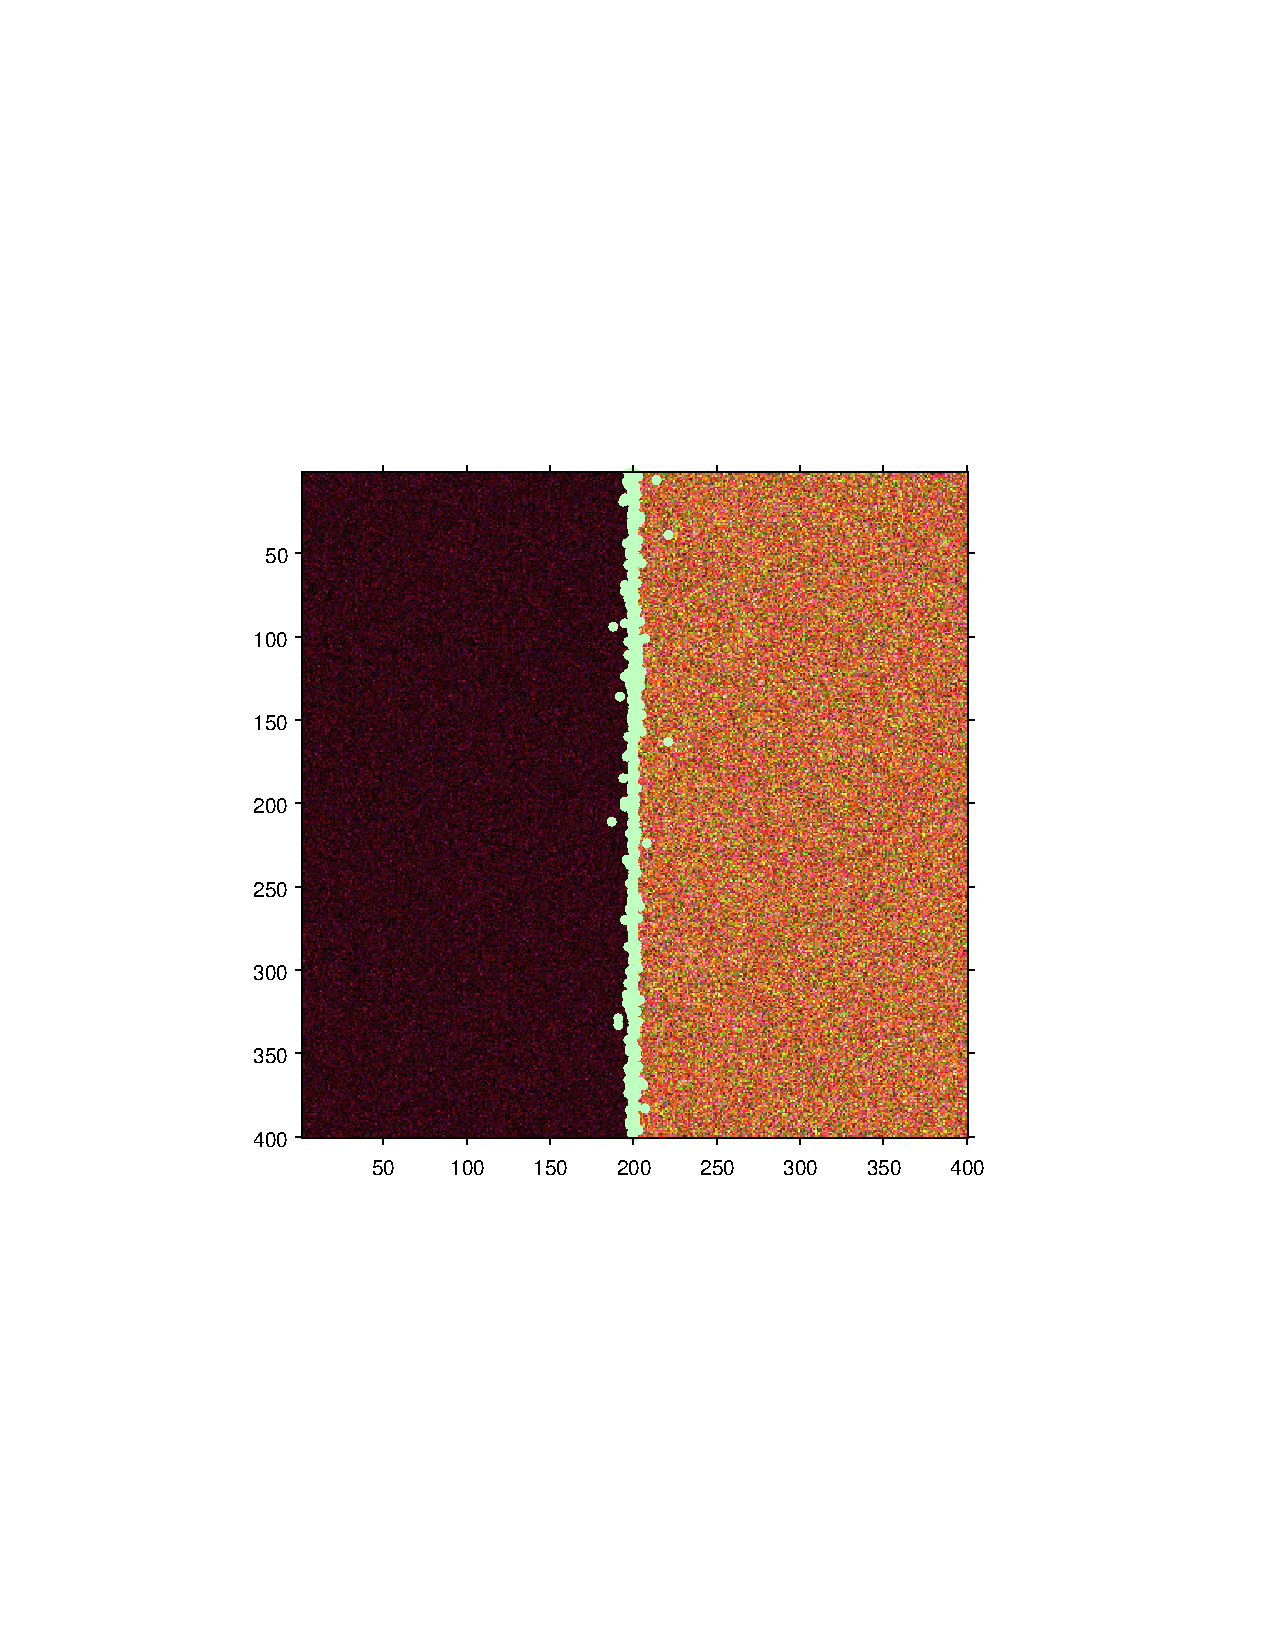
\includegraphics[width=0.5\linewidth]{im_sim_gamf_hv_vv_param_tau_rho_14_pixel}
     }
    \caption{Evidências de bordas para os três canais de intensidade}
     \label{evidencias_hh_hv_vv_gamf} 
   \end{figure*}   
   
   
\subsection{Distribuição bivariada produto de intensidades - Lee } 

Seja a função distribuição de probabilidade 
\begin{equation}\label{func_biv_produto_inten_b1_b2}
	f(B_1,B_2;\rho, L)=\frac{\left(B_1B_2\right)^{\frac{L-1}{2}}\exp\left(-\frac{B_1+B_2}{1-|\rho|^2}\right)}{\Gamma(L)(1-|\rho|^2)|\rho|^{L-1}}I_{L-1}\left(2\sqrt{B_1B_2}\frac{|\rho|}{1-|\rho|^2}\right)
\end{equation}
Considerando as seguintes relações 
\begin{equation}\label{eqn59}
\begin{array}{ccccc}
	R_1&=&\frac{1}{L}\sum_{k=1}^{L}|S_i(k)|^2&=&\frac{B_1\Sigma_{11}}{L}\\
	R_2&=&\frac{1}{L}\sum_{k=1}^{L}|S_j(k)|^2&=&\frac{B_2\Sigma_{22}}{L}\\
\end{array}
\end{equation}
\begin{equation}\label{fun_pdf_biv_inten}
	f(R_1,R_2;\rho,L, \Sigma_{11}, \Sigma_{22})=\frac{L^{L+1}\left(R_1R_2\right)^{\frac{L-1}{2}}\exp\left(-\frac{L\left(\frac{R_1}{\Sigma_{11}}+\frac{R_2}{\Sigma_{22}}\right)}{1-|\rho|^2}\right)}{(\Sigma_{11}\Sigma_{22})^{\frac{L+1}{2}}\Gamma(L)(1-|\rho|^2)|\rho|^{L-1}}I_{L-1}\left(2L\sqrt{\frac{R_1R_2}{\Sigma_{11}\Sigma_{22}}}\frac{|\rho|}{1-|\rho|^2}\right)
\end{equation}

Aplicando o logaritmo natural na equação em ambos os lados da  (\ref{fun_pdf_biv_inten})
\begin{equation}\nonumber
\begin{split}
	\ln f(R_1,R_2;\rho, L, \Sigma_{11}, \Sigma_{22})&=\ln\left(\frac{L^{L+1}\left(R_1R_2\right)^{\frac{L-1}{2}}\exp\left(-\frac{L\left(\frac{R_1}{\Sigma_{11}}+\frac{R_2}{\Sigma_{22}}\right)}{1-|\rho|^2}\right)}{(\Sigma_{11}\Sigma_{22})^{\frac{L+1}{2}}\Gamma(L)(1-|\rho|^2)|\rho_c|^{L-1}}I_{L-1}\left(2L\sqrt{\frac{R_1R_2}{\Sigma_{11}\Sigma_{22}}}\frac{|\rho|}{1-|\rho|^2}\right)\right)\\
	\end{split}
\end{equation}
\begin{equation}\nonumber
\begin{split}
	\ln f(R_1,R_2;\rho,L, \Sigma_{11}, \Sigma_{22})&=\ln\left(\frac{L^{L+1}\left(R_1R_2\right)^{\frac{L-1}{2}}\exp\left(-\frac{L\left(\frac{R_1}{\Sigma_{11}}+\frac{R_2}{\Sigma_{22}}\right)}{1-|\rho|^2}\right)}{(\Sigma_{11}\Sigma_{22})^{\frac{L+1}{2}}\Gamma(L)(1-|\rho|^2)|\rho|^{L-1}}\right)
	 +\ln I_{L-1}\left(2L\sqrt{\frac{R_1R_2}{\Sigma_{11}\Sigma_{22}}}\frac{|\rho|}{1-|\rho|^2}\right)\\
	             &=\ln\left(L^{L+1}\left(R_1R_2\right)^{\frac{L-1}{2}}\exp\left(-\frac{L\left(\frac{R_1}{\Sigma_{11}}+\frac{R_2}{\Sigma_{22}}\right)}{1-|\rho|^2}\right)\right)-\ln\left((\Sigma_{11}\Sigma_{22})^{\frac{L+1}{2}}\Gamma(L)(1-|\rho|^2)|\rho|^{L-1}\right) \\
	&+\ln I_{L-1}\left(2L\sqrt{\frac{R_1R_2}{\Sigma_{11}\Sigma_{22}}}\frac{|\rho|}{1-|\rho|^2}\right)
	\end{split}
\end{equation}
\begin{equation}\nonumber
\begin{split}
	\ln f(R_1,R_2;\rho,L, \Sigma_{11}, \Sigma_{22})&=\ln\left(L^{L+1}\left(R_1R_2\right)^{\frac{L-1}{2}}\right) + \ln \exp\left(-\frac{L\left(\frac{R_1}{\Sigma_{11}}+\frac{R_2}{\Sigma_{22}}\right)}{1-|\rho|^2}\right)-\ln\left((\Sigma_{11}\Sigma_{22})^{\frac{L+1}{2}}\Gamma(L)(1-|\rho|^2)|\rho|^{L-1}\right) \\
	&+\ln I_{L-1}\left(2L\sqrt{\frac{R_1R_2}{\Sigma_{11}\Sigma_{22}}}\frac{|\rho|}{1-|\rho|^2}\right)\\
	&=\ln L^{L+1} + \ln (R_1R_2)^{\frac{L-1}{2}} -\frac{L\left(\frac{R_1}{\Sigma_{11}}+\frac{R_2}{\Sigma_{22}}\right)}{1-|\rho|^2}-\ln(\Sigma_{11}\Sigma_{22})^{\frac{L+1}{2}} - \ln\Gamma(L)- \ln(1-|\rho|^2)-\ln|\rho|^{L-1} \\
	&+\ln I_{L-1}\left(2L\sqrt{\frac{R_1R_2}{\Sigma_{11}\Sigma_{22}}}\frac{|\rho|}{1-|\rho|^2}\right)\\
	&=(L+1)\ln L +\frac{L-1}{2} \ln (R_1R_2) -\frac{LR_1}{\Sigma_{11}(1-|\rho|^2)}-\frac{LR_2}{\Sigma_{22}(1-|\rho|^2)}\\
	&-\frac{L+1}{2}\ln(\Sigma_{11}\Sigma_{22}) - \ln\Gamma(L)- \ln(1-|\rho|^2)-(L-1)\ln|\rho|\\
	&+\ln I_{L-1}\left(2L\sqrt{\frac{R_1R_2}{\Sigma_{11}\Sigma_{22}}}\frac{|\rho|}{1-|\rho|^2}\right)
\end{split}
\end{equation}
	 	
\begin{equation}\label{fun_log_biv_inten}
\begin{split}
	\ln f(R_1,R_2;\rho,L, \Sigma_{11}, \Sigma_{22})&=(L+1)\ln L +\frac{L-1}{2} \ln R_1 +\frac{L-1}{2} \ln R_2 -\frac{LR_1}{\Sigma_{11}(1-|\rho|^2)}-\frac{LR_2}{\Sigma_{22}(1-|\rho|^2)}\\
	&-\frac{L+1}{2}\ln\Sigma_{11}-\frac{L+1}{2}\ln\Sigma_{22} - \ln\Gamma(L)- \ln(1-|\rho|^2)-(L-1)\ln|\rho|\\
	&+\ln I_{L-1}\left(2L\sqrt{\frac{R_1R_2}{\Sigma_{11}\Sigma_{22}}}\frac{|\rho|}{1-|\rho|^2}\right)
\end{split}
\end{equation}


A função log-verossimilhança pode ser deduzida da seguinte maneira, dado a amostra $\bm\mu = (\mu_1,\dots,\mu_n)$, 
\begin{equation}\nonumber
\begin{split}
  \ell(R_1, R_2;\rho, L, \Sigma_{11}, \Sigma_{22})=\ln\prod_{k=1}^{n}f(R_1, R_2;\rho,L, \Sigma_{11}, \Sigma_{22})\\
  \ell(R_1, R_2;\rho, L, \Sigma_{11}, \Sigma_{22})=\sum_{k=1}^{n}\ln f(R_1, R_2;\rho,L, \Sigma_{11}, \Sigma_{22}),
 \end{split}
 \end{equation}
usando a função~\eqref{fun_log_biv_inten} teremos,
\begin{equation}\nonumber
\begin{split}
    \ell(R_1, R_2;\rho, L, \Sigma_{11}, \Sigma_{22})&=\sum_{k=1}^{n}\ln f(R_1, R_2;\rho, L, \Sigma_{11}, \Sigma_{22})\\
                         &=\sum_{k=1}^{n}\left[(L+1)\ln L +\frac{L-1}{2} \ln R_1 +\frac{L-1}{2} \ln R_2 -\frac{LR_1}{\Sigma_{11}(1-|\rho|^2)}-\frac{LR_2}{\Sigma_{22}(1-|\rho|^2)}\right.\\
	&-\frac{L+1}{2}\ln\Sigma_{11}-\frac{L+1}{2}\ln\Sigma_{22} - \ln\Gamma(L)- \ln(1-|\rho|^2)-(L-1)\ln|\rho|\\
	&\left.+\ln I_{L-1}\left(2L\sqrt{\frac{R_1R_2}{\Sigma_{11}\Sigma_{22}}}\frac{|\rho|}{1-|\rho|^2}\right)\right]
 \end{split}
 \end{equation}
 
 \begin{equation}\nonumber
\begin{split} 
  \ell(R_1, R_2;\rho, L, \Sigma_{11}, \Sigma_{22})&=(L+1)\ln L\sum_{k=1}^{n}1 +\frac{L-1}{2}\sum_{k=1}^{n} \ln R_1 +\frac{L-1}{2} \sum_{k=1}^{n}\ln R_2\\
                        &-L\sum_{k=1}^{n}\frac{R_1}{\Sigma_{11}(1-|\rho|^2)}-L\sum_{k=1}^{n}\frac{R_2}{\Sigma_{22}(1-|\rho|^2)}\\
	&-\frac{L+1}{2}\sum_{k=1}^{n}\ln\Sigma_{11}-\frac{L+1}{2}\sum_{k=1}^{n}\ln\Sigma_{22} \\
	&- \ln\Gamma(L)\sum_{k=1}^{n}1- \ln(1-|\rho|^2)\sum_{k=1}^{n}1-(L-1)\ln|\rho|\sum_{k=1}^{n}1\\
	&+\sum_{k=1}^{n}\ln I_{L-1}\left(2L\sqrt{\frac{R_1R_2}{\Sigma_{11}\Sigma_{22}}}\frac{|\rho|}{1-|\rho|^2}\right)
\end{split}
\end{equation}

Definimos a equação log-verossimilhança para a PDF univariada~(\ref{fun_log_biv_inten}).
\begin{equation}\nonumber
\begin{split} 
  \ell(R_1, R_2;\rho, L, \Sigma_{11}, \Sigma_{22})&=n\left[(L+1)\ln L - \ln\Gamma(L)- \ln(1-|\rho|^2)-(L-1)\ln|\rho|\right] \\
                        &+\frac{L-1}{2}\sum_{k=1}^{n} \ln R_1 +\frac{L-1}{2} \sum_{k=1}^{n}\ln R_2\\
                        &-L\sum_{k=1}^{n}\frac{R_1}{\Sigma_{11}(1-|\rho|^2)}-L\sum_{k=1}^{n}\frac{R_2}{\Sigma_{22}(1-|\rho|^2)}\\
	&-\frac{L+1}{2}\sum_{k=1}^{n}\ln\Sigma_{11}-\frac{L+1}{2}\sum_{k=1}^{n}\ln\Sigma_{22} \\
	&+\sum_{k=1}^{n}\ln I_{L-1}\left(2L\sqrt{\frac{R_1R_2}{\Sigma_{11}\Sigma_{22}}}\frac{|\rho|}{1-|\rho|^2}\right)
\end{split}
\end{equation} 
e a forma reduzida,
\begin{equation}\label{eq_log_vero_biv_prod_red}
\begin{split}
\ell(R_1, R_2;\rho, L, \Sigma_{11}, \Sigma_{22})&=n\left[(L+1)\ln L - \ln\Gamma(L)- \ln(1-|\rho|^2)-(L-1)\ln|\rho|\right. \\
	                    &-\left.\frac{L}{2}\ln\Sigma_{11}-\frac{L}{2}\ln\Sigma_{22}\right] \\
                        &+\frac{L}{2}\sum_{k=1}^{n} \ln R_1 +\frac{L}{2} \sum_{k=1}^{n}\ln R_2\\
                        &-\frac{L}{\Sigma_{11}(1-|\rho|^2)}\sum_{k=1}^{n}R_1-\frac{L}{\Sigma_{22}(1-|\rho|^2)}\sum_{k=1}^{n}R_2\\
	&+\sum_{k=1}^{n}\ln I_{L-1}\left(2L\sqrt{\frac{R_1R_2}{\Sigma_{11}\Sigma_{22}}}\frac{|\rho|}{1-|\rho|^2}\right)
\end{split}
 \end{equation} 

Vamos obter $(\widehat \rho, \widehat L)$, o estimador de máxima verossimilhança (MLE) de $(\rho, L)$ baseado $\bm \mu$, por maximizar~\eqref{eq_log_vero_razao_intensidade_red} com o método BFGS implementado no pacote \texttt{maxLik}~\citep{ht}. Vamos preferir otimização resolvendo $\nabla\ell=\bm 0$ com intuito de melhorar a estabilidade numérica.

O função é a log-verossimilhança reduzida para as amostras internas e externas da faixa de dados denotadas respectivamento como $\bm \mu_\text{I}$ e $\bm \mu_\text{E}$. Cada faixa de dados $\bm \mu = (\mu_1,\mu_2,\dots,\mu_n)$ é particionada em duas amostras disjuntas na posição $j$:  
$$
\bm \mu = (\underbrace{\mu_1,\mu_2,\dots,\mu_j}_{\bm \mu_\text{I}}, 
\underbrace{\mu_{j+1}, \mu_{j+2},\dots,\mu_n}_{\bm \mu_\text{E}}).
$$
%Vamos assumir dois diferentes modelos para cada partição:
%$\bm Z_\text{I} \sim \Gamma(\mu_\text{I},L_\text{I})$, e
%$\bm Z_\text{E} \sim \Gamma(\mu_\text{E},L_\text{E})$.
Vamos estimar $(\rho_\text{I},L_\text{I})$ e $(\rho_\text{E},L_\text{E})$ com $\bm \mu_\text{I}$ e $\bm \mu_\text{E}$, respectivamente, maximizando~\eqref{eq:eq_log_vero_mag_prod_red}, e obtendo $(\widehat{\rho}_\text{I}, \widehat{L}_\text{I})$ e $(\widehat{\rho}_\text{E}, \widehat{•}t{L}_\text{E})$.

A log-verossimilhança no ponto $j$ é, então
\begin{equation}\label{eq:TotalLogLikelihood}
\begin{split}
\ell(j;\widehat{\rho}_\text{I}, \widehat{L}_\text{I}, \widehat{\rho}_\text{E}, \widehat{L}_\text{E})&=n\left[(\widehat{L}_\text{I}+1)\ln \widehat{L}_\text{I} - \ln\Gamma(\widehat{L}_\text{I})- \ln(1-|\widehat{\rho}_\text{I}|^2)-(\widehat{L}_\text{I}-1)\ln|\widehat{\rho}_\text{I}|\right] \\
                        &+\frac{\widehat{L}_\text{I}}{2}\sum_{k=1}^{n} \ln R_1 +\frac{\widehat{L}_\text{I}}{2} \sum_{k=1}^{n}\ln R_2\\
                        &-\frac{\widehat{L}_\text{I}}{1-|\widehat{\rho}_\text{I}|^2}\sum_{k=1}^{n}\frac{R_1}{\Sigma_{11}}-\frac{\widehat{L}_\text{I}}{1-|\widehat{\rho}_\text{I}|^2}\sum_{k=1}^{n}\frac{R_2}{\Sigma_{22}}\\
	&-\frac{\widehat{L}_\text{I}}{2}\sum_{k=1}^{n}\ln\Sigma_{11}-\frac{\widehat{L}_\text{I}}{2}\sum_{k=1}^{n}\ln\Sigma_{22} \\
	&+\sum_{k=1}^{n}\ln I_{\widehat{L}_\text{I}-1}\left(2\widehat{L}_\text{I}\sqrt{\frac{R_1R_2}{\Sigma_{11}\Sigma_{22}}}\frac{|\widehat{\rho}_\text{I}|}{1-|\widehat{\rho}_\text{I}|^2}\right)\\
	&+n\left[(\widehat{L}_\text{E}+1)\ln \widehat{L}_\text{E} - \ln\Gamma(\widehat{L}_\text{E})- \ln(1-|\widehat{\rho}_\text{E}|^2)-(\widehat{L}_\text{E}-1)\ln|\widehat{\rho}_\text{E}|\right] \\
                        &+\frac{\widehat{L}_\text{E}}{2}\sum_{k=1}^{n} \ln R_1 +\frac{\widehat{L}_\text{E}}{2} \sum_{k=1}^{n}\ln R_2\\
                        &-\frac{\widehat{L}_\text{E}}{1-|\widehat{\rho}_\text{E}|^2}\sum_{k=1}^{n}\frac{R_1}{\Sigma_{11}}-\frac{\widehat{L}_\text{E}}{1-|\widehat{\rho}_\text{E}|^2}\sum_{k=1}^{n}\frac{R_2}{\Sigma_{22}}\\
	&-\frac{\widehat{L}_\text{E}}{2}\sum_{k=1}^{n}\ln\Sigma_{11}-\frac{\widehat{L}_\text{E}}{2}\sum_{k=1}^{n}\ln\Sigma_{22} \\
	&+\sum_{k=1}^{n}\ln I_{\widehat{L}_\text{E}-1}\left(2\widehat{L}_\text{E}\sqrt{\frac{R_1R_2}{\Sigma_{11}\Sigma_{22}}}\frac{|\widehat{\rho}_\text{E}|}{1-|\widehat{\rho}_\text{E}|^2}\right)
\end{split}
\end{equation}

Vamos aplicar o método GenSA para encontrar
$$
\widehat{\jmath}= \arg\max\limits_{j\in [\min_s,N-\min_s]}\ell(j;\widehat{\rho}_I, \widehat{L}_I,\widehat{\rho}_E, \widehat{L}_E),
$$ 
onde $\min_s$ é o tamanho mínimo da amostra definido por $14$.

Desta maneira, vamos obter uma estimativa para a borda em cada canal de intensidade.
Note que esse método pode ser estendido e/ou modificado para lidar com qualquer tipo de dados.

\section{Resultados numéricos para o método MLE aplicado em cada distribuíção}

Usamos uma imagem AIRSAR PolSAR de Flevoland, banda L, de $750\times 1024$ pixels para os testes.  Fig.~\ref{flevoland_radial_4look} mostra o ROI, com as linhas radiais onde as bordas são detectadas. Fig.~\ref{flevoland_flevoland} mostra a referência do solo em vermelho.  
  \begin{figure}[hbt]
   \centering
     \subfloat[Imagem, Região de Interesse (ROI), and radiais. \label{flevoland_radial_4look}]{%
%       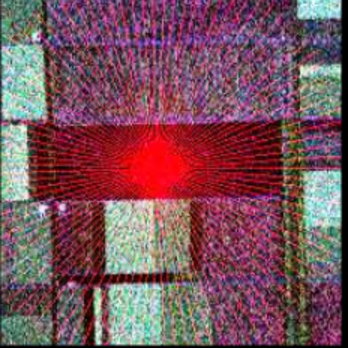
\includegraphics[viewport= 0 50 500 550, clip=true, width=0.23\textwidth]{flevoland_radial_4_look_black_crop}}      
       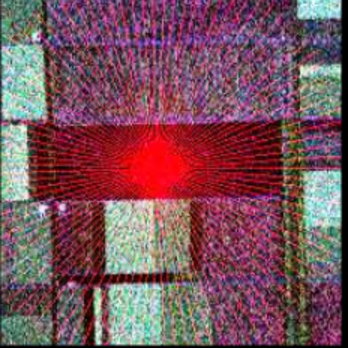
\includegraphics[width=0.53\textwidth]{flevoland_radial_4_look_black_crop}}
     \subfloat[Ground reference\label{gt_flevoland}]{%
       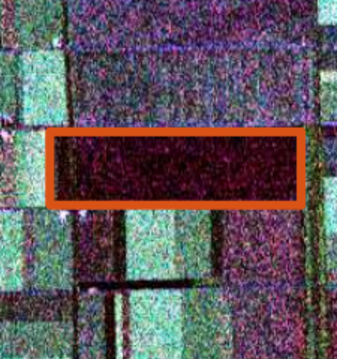
\includegraphics[width=0.5\textwidth]{gt_flevoland_crop}
     }
    \caption{Decomposição de Pauli para a imagem de Flevoland, região de interesse, e referência \textit{ground}}
    \label{roi_gt}
\end{figure}

\subsection{Método da verossimilhança aplicado na pdf univariada $\Gamma$.}
Resolvendo o problema,
$$
\widehat{\jmath}= \arg\max\limits_{j\in [\min_s,N-\min_s]}\ell(j;\widehat{\rho}_I, \widehat{L}_I,\widehat{\rho}_E, \widehat{L}_E),
$$

Figs.~\ref{evidencias_hh_hv_vv}\subref{evidencias_hh_hv_vv:a},~\ref{evidencias_hh_hv_vv}\subref{evidencias_hh_hv_vv:b}, e~\ref{evidencias_hh_hv_vv:a}\subref{evidencias_hh_hv_vv:c}, mostram, respectivamente, as evidências de borda nos canais $\text{hh}$, $\text{hv}$ e $\text{vv}$ como obtidos pela MLE.

Vale notar que a GenSA identificou com precisão o valor máximo de $\eqref{eq:TotalLogLikelihood}$, mesmo na presença de múltiplos máximos locais. 
Uma avaliação visual leva à conclusão de que os melhores resultados são fornecidos por $\text{hv}$, embora com alguns pontos longe da borda real.

 \begin{figure*}[hbt]
	\centering
     \subfloat[Evidências no canal $\text{hh}$ \label{evidencias_hh_hv_vv:a}]{%
       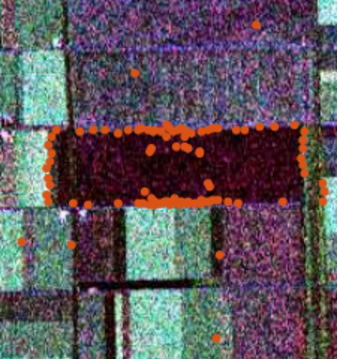
\includegraphics[width=0.32\linewidth]{flevoland_hh_evid_param_L_mu_14_pixel_crop}
     }
     \subfloat[Evidências no canal $\text{hv}$ \label{evidencias_hh_hv_vv:b}]{%
       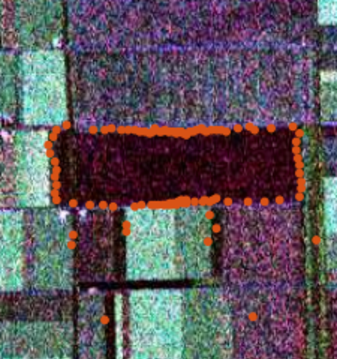
\includegraphics[width=0.32\linewidth]{flevoland_hv_evid_param_L_mu_14_pixel_crop}
     }
     \subfloat[Evidências no canal $\text{vv}$ \label{evidencias_hh_hv_vv:c}]{%
       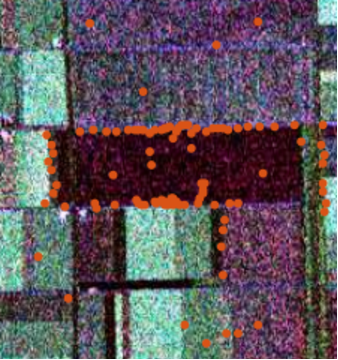
\includegraphics[width=0.32\linewidth]{flevoland_vv_evid_param_L_mu_14_pixel_crop}
     }
     \caption{Evidências de bordas para os três canais de intensidade}
     \label{evidencias_hh_hv_vv} 
   \end{figure*}

\subsection{Método da verossimilhança aplicado na pdf magnitude do produto.}


 \begin{figure*}[hbt]
	\centering
     \subfloat[Evidências no canal $\text{hh}$ \label{evidencias_hh_hv_vv:a}]{%
       \includegraphics[width=0.32\linewidth]{}
     }
     \subfloat[Evidências no canal $\text{hv}$ \label{evidencias_hh_hv_vv:b}]{%
       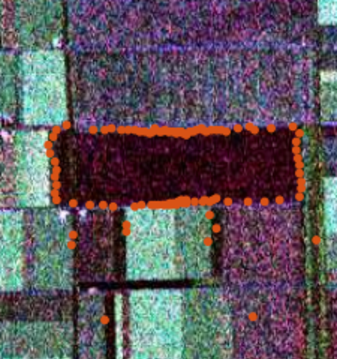
\includegraphics[width=0.32\linewidth]{flevoland_hv_evid_param_L_mu_14_pixel_crop}
     }
     \subfloat[Evidências no canal $\text{vv}$ \label{evidencias_hh_hv_vv:c}]{%
       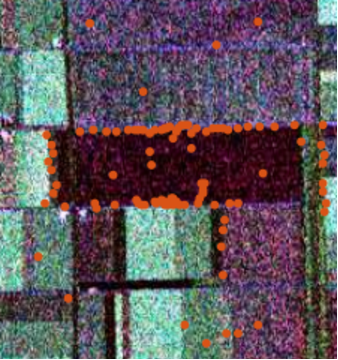
\includegraphics[width=0.32\linewidth]{flevoland_vv_evid_param_L_mu_14_pixel_crop}
     }
     \caption{Evidências de bordas para os três canais de intensidade}
     \label{evidencias_hh_hv_vv} 
   \end{figure*}


%\begin{figure}[hbt]
%\minipage{0.5\textwidth}
%  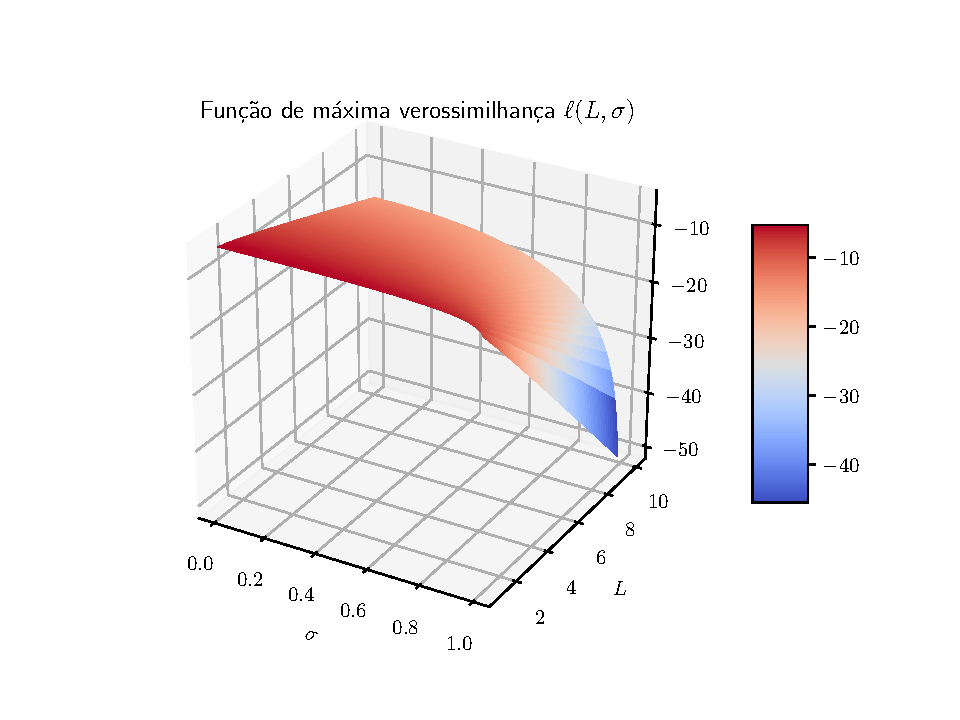
\includegraphics[width=\linewidth]{funv_max_ver_j_10_flev_razao.pdf}
%  	\caption{$\sigma= 12.3426$.}\label{cap_acf_fig04}
%\endminipage\hfill
%\minipage{0.5\textwidth}
%  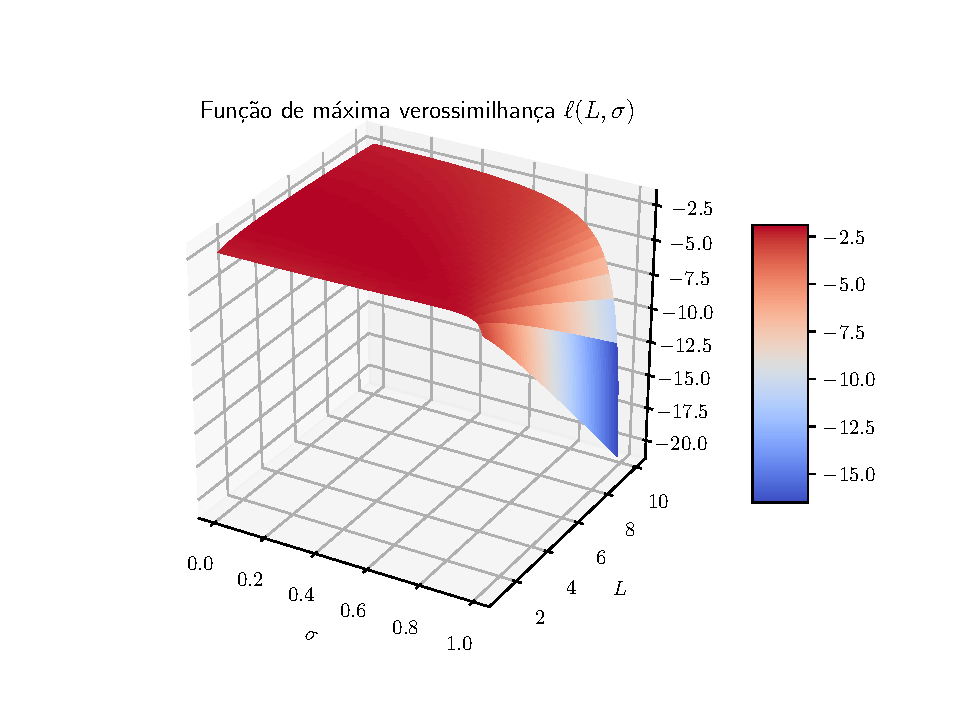
\includegraphics[width=\linewidth]{funv_max_ver_j_20_flev_razao.pdf}
%		\caption{$\sigma=2.1029 $.}\label{cap_acf_fig05}
%\endminipage\hfill
%\centering
%\minipage{0.5\textwidth}
%  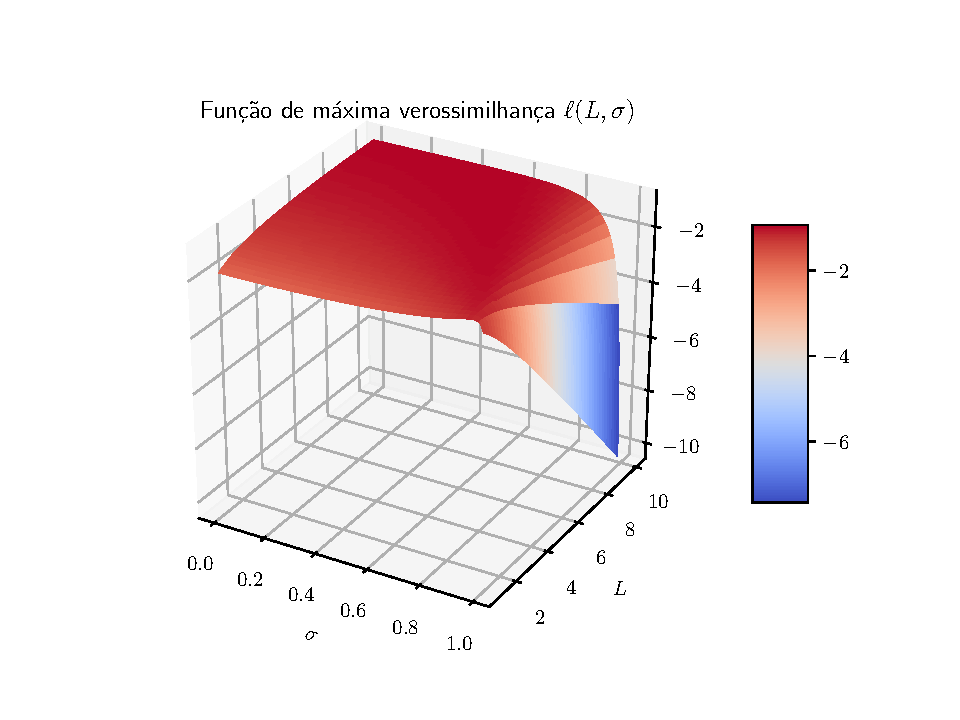
\includegraphics[width=\linewidth]{funv_max_ver_j_30_flev_razao.pdf}
%  	\caption{$\sigma=1.4999 $.}\label{cap_acf_fig04}
%\endminipage\hfill
%\minipage{0.5\textwidth}
%  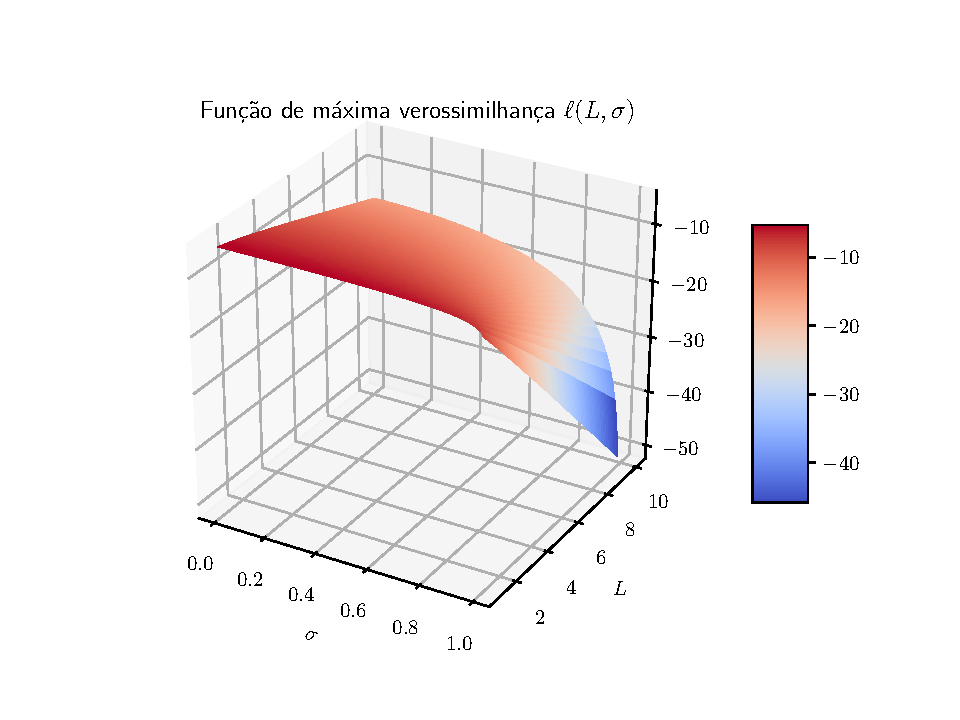
\includegraphics[width=\linewidth]{funv_max_ver_j_40_flev_razao.pdf}
%		\caption{$\sigma=12.6414 $.}\label{cap_acf_fig05}
%\endminipage\hfill
%\end{figure}
%\begin{figure}[hbt]
%\minipage{0.5\textwidth}
%  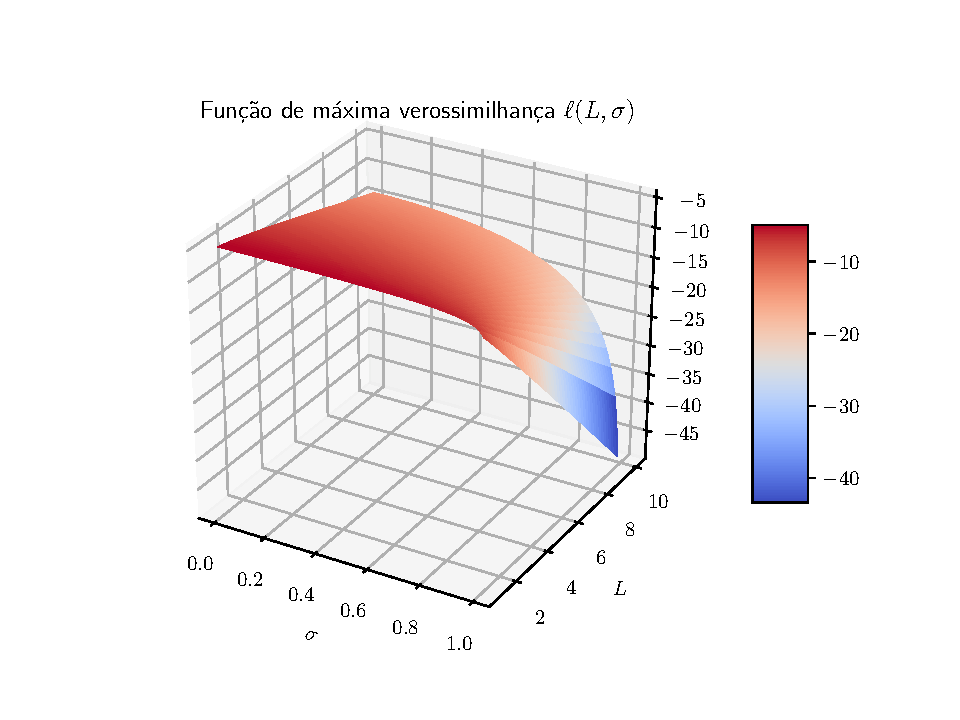
\includegraphics[width=\linewidth]{funv_max_ver_j_50_flev_razao.pdf}
%  	\caption{$\sigma=10.4523$.}\label{cap_acf_fig04}
%\endminipage\hfill
%\minipage{0.5\textwidth}
%  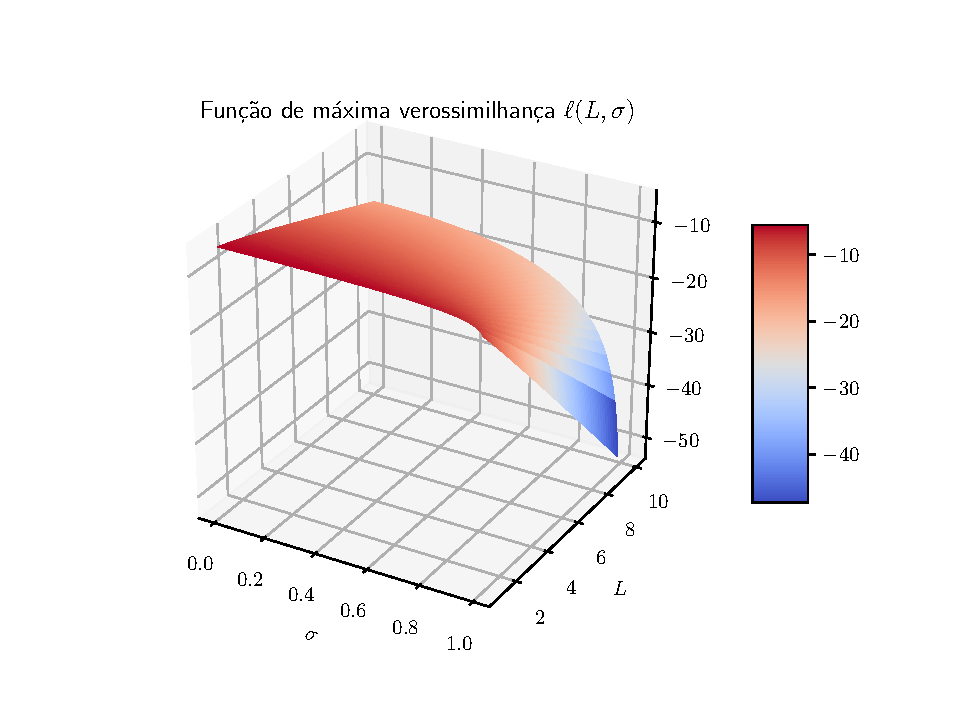
\includegraphics[width=\linewidth]{funv_max_ver_j_60_flev_razao.pdf}
%		\caption{$\sigma= 14.2156$.}\label{cap_acf_fig05}
%\endminipage\hfill
%\centering
%\minipage{0.5\textwidth}
%  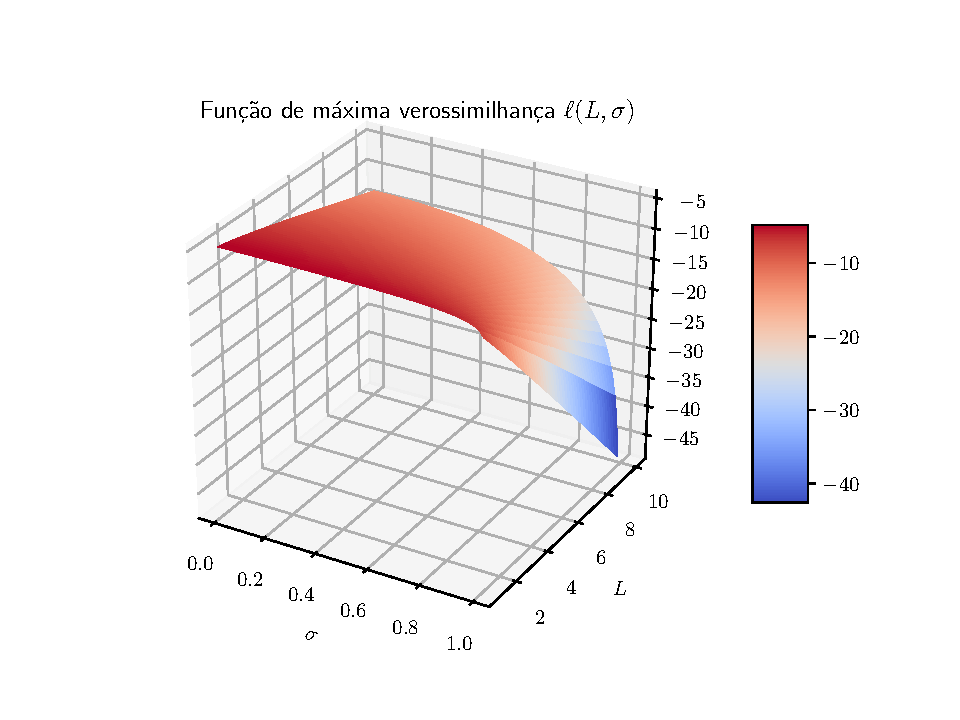
\includegraphics[width=\linewidth]{funv_max_ver_j_70_flev_razao.pdf}
%  	\caption{$\sigma=9.8405 $.}\label{cap_acf_fig04}
%\endminipage\hfill
%\minipage{0.5\textwidth}
%  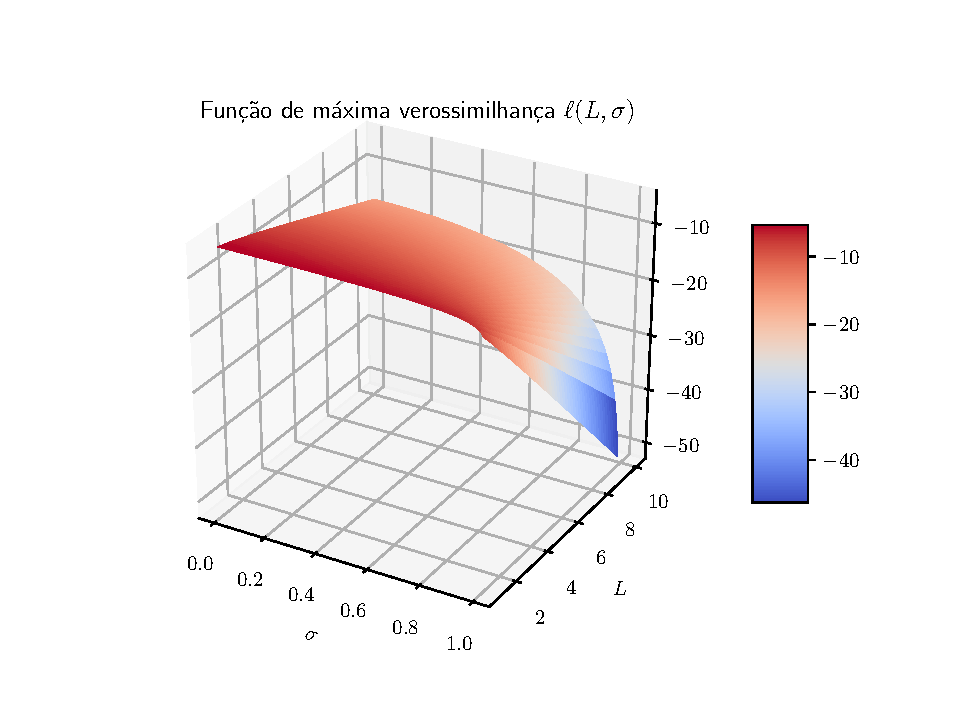
\includegraphics[width=\linewidth]{funv_max_ver_j_80_flev_razao.pdf}
%		\caption{$\sigma=13.1298 $.}\label{cap_acf_fig05}
%\endminipage\hfill
%\end{figure}
%\subsection{Distribuição univariada da magnitude do produto}
%A magnitude do produto $\mathbf{S}_i$ e $\mathbf{S}_j$ é uma importante medida para as imagem SAR polarimétrica. Definimos a magnitude normalizada por 
%
%\begin{equation}
%	\xi = \frac{\left|\frac{1}{L} \sum_{k=1}^L\mathbf{S}_i(k)\mathbf{S}_j^H(k) \right|}{\sqrt{E[|\mathbf{S}_i|^2]E[|\mathbf{S}_i|^2]}}=\frac{g}{h}.
%\end{equation}
%onde é definido por $g=|\mathbf{S}_i\mathbf{S}_j^H|$ e $h=\sqrt{E[|\mathbf{S}_i|^2]E[|\mathbf{S}_i|^2]}$.
%\begin{equation}
%\begin{array}{ccc}
%	f(\xi)&=&\frac{4L^{L+1}\xi^L}{\Gamma(L)(1-|\rho|^2)}I_0\left(\frac{2|\rho|L\xi}{1-|\rho|^2}\right)K_{L-1}\left(\frac{2L\xi}{1-|\rho|^2}\right).
%		\end{array}
%\end{equation}
%\begin{equation}
%\begin{array}{ccc}
%	\ln f(\xi)&=&\ln\left(\frac{4L^{L+1}\xi^L}{\Gamma(L)(1-|\rho|^2)}I_0\left(\frac{2|\rho|L\xi}{1-|\rho|^2}\right)K_{L-1}\left(\frac{2L\xi}{1-|\rho|^2}\right)\right).
%		\end{array}
%\end{equation}
%\begin{equation}
%\begin{array}{ccc}
%	\ln f(\xi)&=&\ln\left(\frac{4L^{L+1}\xi^L}{\Gamma(L)(1-|\rho|^2)}\right)+\ln I_0\left(\frac{2|\rho|L\xi}{1-|\rho|^2}\right)+ \ln K_{L-1}\left(\frac{2L\xi}{1-|\rho|^2}\right).
%		\end{array}
%\end{equation}
%
%\begin{equation}
%\begin{array}{ccc}
%	\ln f(\xi)&=&\ln (4L^{L+1}\xi^L)-\ln(\Gamma(L)(1-|\rho|^2))+\ln I_0\left(\frac{2|\rho|L\xi}{1-|\rho|^2}\right)+ \ln K_{L-1}\left(\frac{2L\xi}{1-|\rho|^2}\right).
%		\end{array}
%\end{equation}
%
%\begin{equation}
%\begin{array}{ccc}
%	\ln f(\xi)&=&\ln (4)+\ln L^{L+1}+\ln \xi^L-\ln\Gamma(L)-\ln(1-|\rho|^2)+\ln I_0\left(\frac{2|\rho|L\xi}{1-|\rho|^2}\right)+ \ln K_{L-1}\left(\frac{2L\xi}{1-|\rho|^2}\right).
%		\end{array}
%\end{equation}
%
%\begin{equation}
%\begin{array}{ccc}
%	\ln f(\xi)&=&\ln (4)+(L+1)\ln L+L\ln \xi-\ln\Gamma(L)-\ln(1-|\rho|^2)+\ln I_0\left(\frac{2|\rho|L\xi}{1-|\rho|^2}\right)+ \ln K_{L-1}\left(\frac{2L\xi}{1-|\rho|^2}\right).
%		\end{array}
%\end{equation}
%
%\begin{figure}[hbt]
%\minipage{0.5\textwidth}
%  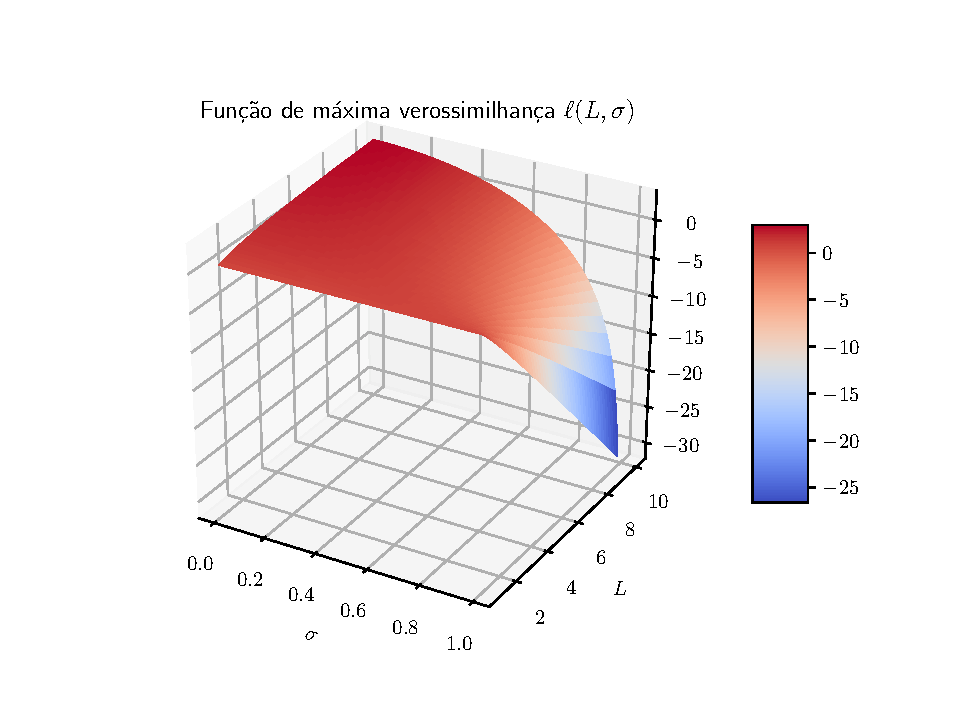
\includegraphics[width=\linewidth]{funv_max_ver_j_10_flev_produto.pdf}
%  	\caption{$\sigma= 0.0001241$.}\label{cap_acf_fig04}
%\endminipage\hfill
%\minipage{0.5\textwidth}
%  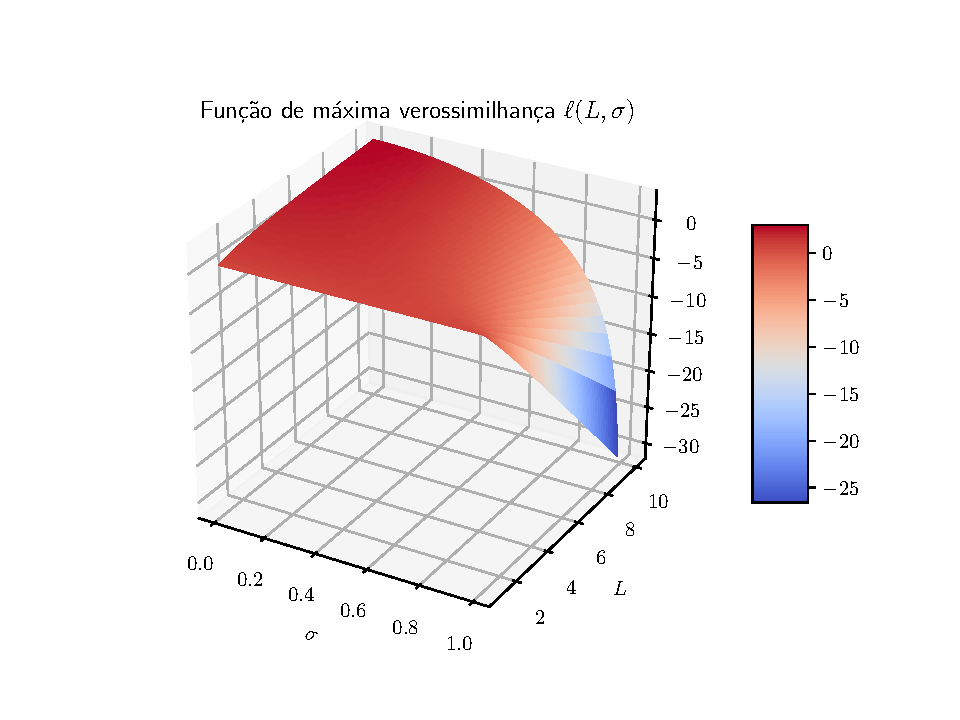
\includegraphics[width=\linewidth]{funv_max_ver_j_20_flev_produto.pdf}
%		\caption{$\sigma= 0.0021969$.}\label{cap_acf_fig05}
%\endminipage\hfill
%\centering
%\minipage{0.5\textwidth}
%  \includegraphics[width=\linewidth]{funv_max_ver_j_30_flev_produto.pdf}
%  	\caption{$\sigma=0.0047520 $.}\label{cap_acf_fig04}
%\endminipage\hfill
%\minipage{0.5\textwidth}
%  \includegraphics[width=\linewidth]{funv_max_ver_j_40_flev_produto.pdf}
%		\caption{$\sigma= 0.0123943$.}\label{cap_acf_fig05}
%\endminipage\hfill
%\end{figure}
%\begin{figure}[hbt]
%\minipage{0.5\textwidth}
%  \includegraphics[width=\linewidth]{funv_max_ver_j_50_flev_produto.pdf}
%  	\caption{$\sigma= 0.0002715$.}\label{cap_acf_fig04}
%\endminipage\hfill
%\minipage{0.5\textwidth}
%  \includegraphics[width=\linewidth]{funv_max_ver_j_60_flev_produto.pdf}
%		\caption{$\sigma= 0.0001922$.}\label{cap_acf_fig05}
%\endminipage\hfill
%\centering
%\minipage{0.5\textwidth}
%  \includegraphics[width=\linewidth]{funv_max_ver_j_70_flev_produto.pdf}
%  	\caption{$\sigma= 0.0004329$.}\label{cap_acf_fig04}
%\endminipage\hfill
%\minipage{0.5\textwidth}
%  \includegraphics[width=\linewidth]{funv_max_ver_j_80_flev_produto.pdf}
%		\caption{$\sigma= 0.0002790$.}\label{cap_acf_fig05}
%\endminipage\hfill
%\end{figure}


%\subsection{Distribuição bivariada produto de intensidades - Lee } 
%
%O $PDF$ conjunto retorna de dois canais correlacionados dos radares polarimétricos e interferométricos são importantes. As $PDF's$ conjuntas conduzem a derivação da intensidade e amplitude razão $PDF's$. Da equação (\ref{eqn42}) temos que as intensidades {\it multilook} sejam 
%
%\begin{equation}\label{eqn59}
%\begin{array}{ccccc}
%	R_1&=&\frac{1}{n}\sum_{k=1}^{n}|S_i(k)|^2&=&\frac{B_1C_{11}}{n}\\
%	R_2&=&\frac{1}{n}\sum_{k=1}^{n}|S_j(k)|^2&=&\frac{B_2C_{22}}{n}\\
%\end{array}
%\end{equation}
%
%Integrando a equação (\ref{eqn52}) em relação a $\eta$ e $\psi$. A $PDF$ é
%
%\begin{equation}\label{eqn60}
%	p(B_1,B_2)=\frac{\left(B_1B_2\right)^{\frac{n-1}{2}}\exp\left(-\frac{B_1+B_2}{1-|\rho_c|^2}\right)}{\Gamma(n)(1-|\rho_c|^2)|\rho_c|^{n-1}}I_{n-1}\left(2\sqrt{B_1B_2}\frac{|\rho_c|}{1-|\rho_c|^2}\right)
%\end{equation}

%Sendo
%\begin{equation}\label{eqn61}
%	I_{\mu}(Z)=\frac{(\frac{z}{2})^{\mu}}{\Gamma(\mu+1)} F_{1}^{0}[-;\mu+1;\frac{z^2}{4}]
%\end{equation}
%
%\begin{equation}\label{eqn62}
%	p(B_1,B_2)=\frac{n^{n+1}\left(R_1R_2\right)^{\frac{n-1}{2}}\exp\left(-\frac{n(\frac{R_1}{C_{11}}+\frac{R_2}{C_{22}})}{1-|\rho_c|^2}\right)}{(C_{11}C_{22})^{\frac{n+1}{2}}\Gamma(n)(1-|\rho_c|^2)|\rho_c|^{n-1}}I_{n-1}\left(2n\sqrt{\frac{R_1R_2}{C_{11}C_{22}}}\frac{|\rho_c|}{1-|\rho_c|^2}\right)
%\end{equation}
%\subsection{Distribuição $\Gamma$ trivariada - Hagedorn }
%\begin{equation}\label{eqn62}
%\begin{array}{ccc}
%	p(I_1,I_2,I_3)&=& \frac{\exp(-\frac{1}{2}(a_1I_1+b_1I_2+c_1I_3))}{8(n-1)|C|^{\frac{n}{2}}(d_1d_2d_3)^{n-1}}\sum_{k=n-1}^{\infty}k(-1)^{k-n+1}C_{k-n+1}^{n-1}(cos(\gamma))\\
%	&&I_k(d_1\sqrt{I_1I_2})I_k(d_2\sqrt{I_2I_3})I_k(d_3\sqrt{I_1I_3})
%\end{array}
%\end{equation}
%
%
%
%Para cada $i$:
%  
%Estimar $(\mu_i, L_i )$ por $(\hat{\mu}_i, \hat{L}_i)(Z_I)$ em uma primeira metade da faixa de dados.
%
%Estimar $(\mu_i, L_i )$ por $(\hat{\mu}_i, \hat{L}_i)(Z_E)$ em uma segunda metade da faixa de dados.
%
%Usando o estimador de máxima verossimilhança, 
%\begin{equation}\label{cap_acf_16}
%    (\hat{\mu}_i, \hat{L}_i)(Z_{\bigodot})= \text{arg}\,\max\limits_{(\mu, L)\in \mathbb{R}^{+}\times \mathbb{R}^{+}}%\ell(\mu,L;Z_i).\\
%\end{equation}
%Assim
%\begin{equation}\label{cap_acf_16}
%\begin{array}{ccc}
% \ell(\mu, L)&=&\ln\left(\prod_{k=1}^{n}f_{Z_{i}}(Z_{k};\mu,L)\right)\\
%  \ell(\mu, L)&=&\sum_{k=1}^{n}\ln\left(f_{Z_{i}}(Z_{k};\mu,L)\right)
% \end{array}
% \end{equation}
%Temos duas amostras
%\begin{equation}\label{cap_acf_16}
% \begin{array}{lll}
%\ell(\mu_I, L_I,\mu_E, L_E, j)&=&\sum_{k=1}^{j}     \left[   L_I\ln L_I +(L_I   - 1) \ln Z_{i}-L_I \ln \mu_I-\ln \Gamma(L_i) -%\frac{L_I}{\mu_I} Z_i \right]\\
%                                               &+&\sum_{k=j+1}^{N}\left[   L_E\ln L_E +(L_E - 1) \ln Z_{i}-L_E \ln \mu_E-\ln \Gamma(L_E) -\frac{L_E}{\mu_E} Z_i \right]\\
%\ell(\mu_I, L_I,\mu_E, L_E, j)&=&  L_I\ln L_I \sum_{k=1}^{j} 1 +(L_I   - 1) \sum_{k=1}^{j}  \ln Z_{i}-L_I \ln \mu_I\sum_{k=1}^{j} 1-\ln \Gamma(L_i) \sum_{k=1}^{j} 1  -\frac{L_I}{\mu_I} \sum_{k=1}^{j}   Z_i \\
%                                               &+&  L_E\ln L_E \sum_{k=j+1}^{N}1+(L_E - 1) \sum_{k=j+1}^{N}\ln Z_{i}- \ln %\mu_E\sum_{k=j+1}^{N}1-\ln \Gamma(L_E)\sum_{k=j+1}^{N} 1-\frac{L_E}{\mu_E} \sum_{k=j+1}^{N}Z_i \\
%\ell(\mu_I, L_I,\mu_E, L_E, j)&=&  L_I\ln L_I j-L_I \ln \mu_I j-\ln \Gamma(L_i) j \\
%&+& (L_I  - 1) \sum_{k=1}^{j}  \ln Z_{i}  -\frac{L_I}{\mu_I} \sum_{k=1}^{j}   Z_i \\
%                                               &+&  L_E\ln L_E (N-j)-L_E \ln \mu_E(N-j)-\ln \Gamma(L_E)(N-j)- \\
%                                               &+& (L_E - 1) \sum_{k=j+1}^{N}\ln Z_{i}-\frac{L_E}{\mu_E} \sum_{k=j+1}^{N}Z_i \\
%                                                \end{array}
% \end{equation}
%
%
%\section{Imagens PolSAR reais}
%\begin{figure}[hbt]
%\centering
%\includegraphics[width=4.0in]{grafico_pdf_lee_1994_razao_amplitude.pdf}
%	\caption{Distribuição razão de amplitudes {\it L- visadas}.}
%\label{fig2}
%\end{figure}
%\begin{figure}[hbt]
%\centering
%	\includegraphics[width=4.0in]{sf_amostras_b_r_y.pdf}
%	\vspace{-2.5cm}
%	\caption{Regiões de interesses (ROIs).}
%\label{fig2}
%\end{figure}
% A tabela mostra os coeficientes de correlação para as regiões destacadas na figura. Os coeficientes correlacionam os canais $(hh-hv)$, $(hh-vv)$ e $(vv-hv)$ respectivamente para o mar ( ROI azul), floresta (ROI vermelho) e zona urbana (ROI amarelo).
%\begin{table}[hbt]
%	\centering
%	\caption{Coeficientes de correlação.}\label{cap_acf_tab04}
%\begin{tabular}{@{}lccc@{}} \toprule
%	Coeficiente de correlação & Mar  & Floresta & Zona urbana \\ \midrule
%	$(hh-hv)$ & 0.5548 & 0.7024 &  0.7177 \\ 
%	$(hh-vv)$ & 0.8743 & 0.6633 &  0.6483\\ 
%	$(vv-hv)$ & 0.5128 & 0.6065 &  0.6175\\ \bottomrule
%\end{tabular}
%\end{table}
%
%A figura acima mostra a baía de San Francisco ($450 \times 600$) com três regiões de interesses destacadas oceâno, floresta e zona urbana respectivamente nas cores azul, vermelho e amarelo. As ROI's têm dimensão ($50 \times 50$) adquirindo dados nos três canais de intensidade. O histograma e as pdf's teóricas são mostradas na figura abaixo. No cálculo das pdf's foi usado a equação 
%\begin{equation}\label{cap_acf_23}
%	f_{Z_{i}}(Z_{i};\frac{L}{\sigma_{i}^2},L)=\frac{L^{L}Z_{i}^{L-1}}{\sigma_{i}^{2L}\Gamma(L)} \exp(-L\frac{Z_{i}}{\sigma_{i}^2}), \\
%\end{equation}
%sendo $L=\{2,3,4\}$ e $\sigma_{i}^2$ a média de todos as entradas das respectivas regiões de interesses conforme \cite{nhfc}.
%
%\begin{figure}[hbt]
%\centering
%	\includegraphics[width=4.0in]{graf_pdf_roi_mar_hh.pdf}
%	\caption{Regiões de interesses (ROIs).}
%\label{fig2}
%\end{figure}
%\textcolor{red}{OBS: Tem algo errado no gráfico, provavelmente a estimativa de $\sigma_{i}$.}
% ****************************************************************
